\pdfoutput=1

\documentclass{l4proj}

%
% put any packages here
%
%\usepackage[demo]{graphicx}
\usepackage{subcaption}

% For producing Python Code Listings
% ----------------------------------

\usepackage{listings}
\usepackage{color}
\usepackage{xcolor}

\lstdefinelanguage{swift}
{
  morekeywords={
    func,if,then,else,for,in,while,do,switch,case,default,where,break,continue,fallthrough,return,
    typealias,struct,class,enum,protocol,var,func,let,get,set,willSet,didSet,inout,init,deinit,extension,
    subscript,prefix,operator,infix,postfix,precedence,associativity,left,right,none,convenience,dynamic,
    final,lazy,mutating,nonmutating,optional,override,required,static,unowned,safe,weak,internal,
    private,public,is,as,self,unsafe,dynamicType,true,false,nil,Type,Protocol,
  },
  morecomment=[l]{//}, % l is for line comment
  morecomment=[s]{/*}{*/}, % s is for start and end delimiter
  morestring=[b]" % defines that strings are enclosed in double quotes
}

\definecolor{keyword}{HTML}{BA2CA3}
\definecolor{string}{HTML}{D12F1B}
\definecolor{comment}{HTML}{008400}

\lstset{
  language=swift,
  basicstyle=\ttfamily,
  showstringspaces=false, % lets spaces in strings appear as real spaces
  columns=fixed,
  keepspaces=true,
  keywordstyle=\color{keyword},
  stringstyle=\color{string},
  commentstyle=\color{comment},
}

\definecolor{dkgreen}{rgb}{0,0.6,0}
\definecolor{gray}{rgb}{0.5,0.5,0.5}
\definecolor{mauve}{rgb}{0.58,0,0.82}

\lstset{frame=tb,
  language=Python,
  aboveskip=3mm,
  belowskip=3mm,
  showstringspaces=false,
  columns=flexible,
  basicstyle={\small\ttfamily},
  numbers=none,
  numberstyle=\tiny\color{gray},
  keywordstyle=\color{blue},
  commentstyle=\color{dkgreen},
  stringstyle=\color{mauve},
  breaklines=true,
  breakatwhitespace=true,
  tabsize=3
}

% ----------------------------------

\begin{document}
\title{Using Machine Learning to Understand the Topology of Knots}
\author{Joseph Manfredi Cameron}
\date{March 28, 2018}
\maketitle

\begin{abstract}
Knots are extremely useful constructs for achieving specific tasks in many industries and applications.
Furthermore, an individual knot can be uniquely identified by its topology.
This dissertation explores the use of machine learning techniques to fully understand knots and their topology by detailing the design and development of an image classifier implemented with convolutional neural networks.
The image classifier was capable of robustly classifying ten individual knots from photos.
Subsequently, the image classifier was then integrated into an iOS application, and the resulting iOS application was capable of classifying knots in real-time.
Further evaluation then showed that the iOS application could classify ten specified knots with an accuracy of 77.5\%.
\end{abstract}

\educationalconsent
%
%NOTE: if you include the educationalconsent (above) and your project is graded an A then
%      it may be entered in the CS Hall of Fame
%
\tableofcontents
%==============================================================================

% INTRODUCTION

\chapter{Introduction}
\pagenumbering{arabic}

Knots have played a vital role throughout human history to achieve a multitude of tasks. 
In ancient times, the use and development of knots contributed to fundamental advances in agriculture, transport and construction.
Thus, knots have played a pivotal role in advancing human civilisation into the modern era.
For example, many sea-going empires and civilisations relied on knots to satisfy a variety of requirements on ships.
Hence, an overwhelming majority of knots, such as those found in the Ashley Book of Knots, were created by sailors and categorised with respect to their appropriate use.
These categories show an abundance of differing properties knots possess due to their topology.
 
Today, knots are still extremely useful in agriculture, science and recreation among many other fields. 
With such a wide array of knots still in use, it is important to be able to classify and fully understand these individual knots and their properties. 
For example, knots are commonly used in mountain climbing, where the life of a climber may depend on the properties of a knot that is tied in climbing rope. 
In situations such as this, it would be beneficial to automatically identify/classify the knot as a means of checking if the correct knot has been tied or not. 
In addition, if the correct knot has not been tied, or it has been tied to an incorrect tension, it may also be useful to show how to fix these errors. 
With the application of machine learning, specifically deep learning, the three-dimensional topology of knots may be better understood to provide such usability. 
Furthermore, a neural network could begin to recover and analyse the topology of a knot in order to provide extra insight as to why certain knots display certain properties.

\section{Aims \& Motivations}
The main aim of this project is to develop deep learning software that can classify individual knots solely from images.
Another aim of this project is to provide a usable interface, through which users can classify knots. 
The classification will be accomplished through the use of a convolutional neural network (CNN). 
Furthermore, the project will include software that can automate the creation and management of image datasets that can be used to train each individual neural network. 
Deep learning visualisation techniques, such as the use of the t-SNE algorithm, will be used to display representations learned by the neural networks and evaluate the effectiveness of the deep learning tasks. 
There will also be significant analysis into what techniques, neural network models and training data help or hinder the accuracy and effectiveness of the deep learning tasks.
Finally, an iOS application will be created to act as an effective interface through which users can classify knots.
An example of the finished application's interface is shown in Figure \ref{fig:IntroApp}.

\begin{figure}
	\centering
	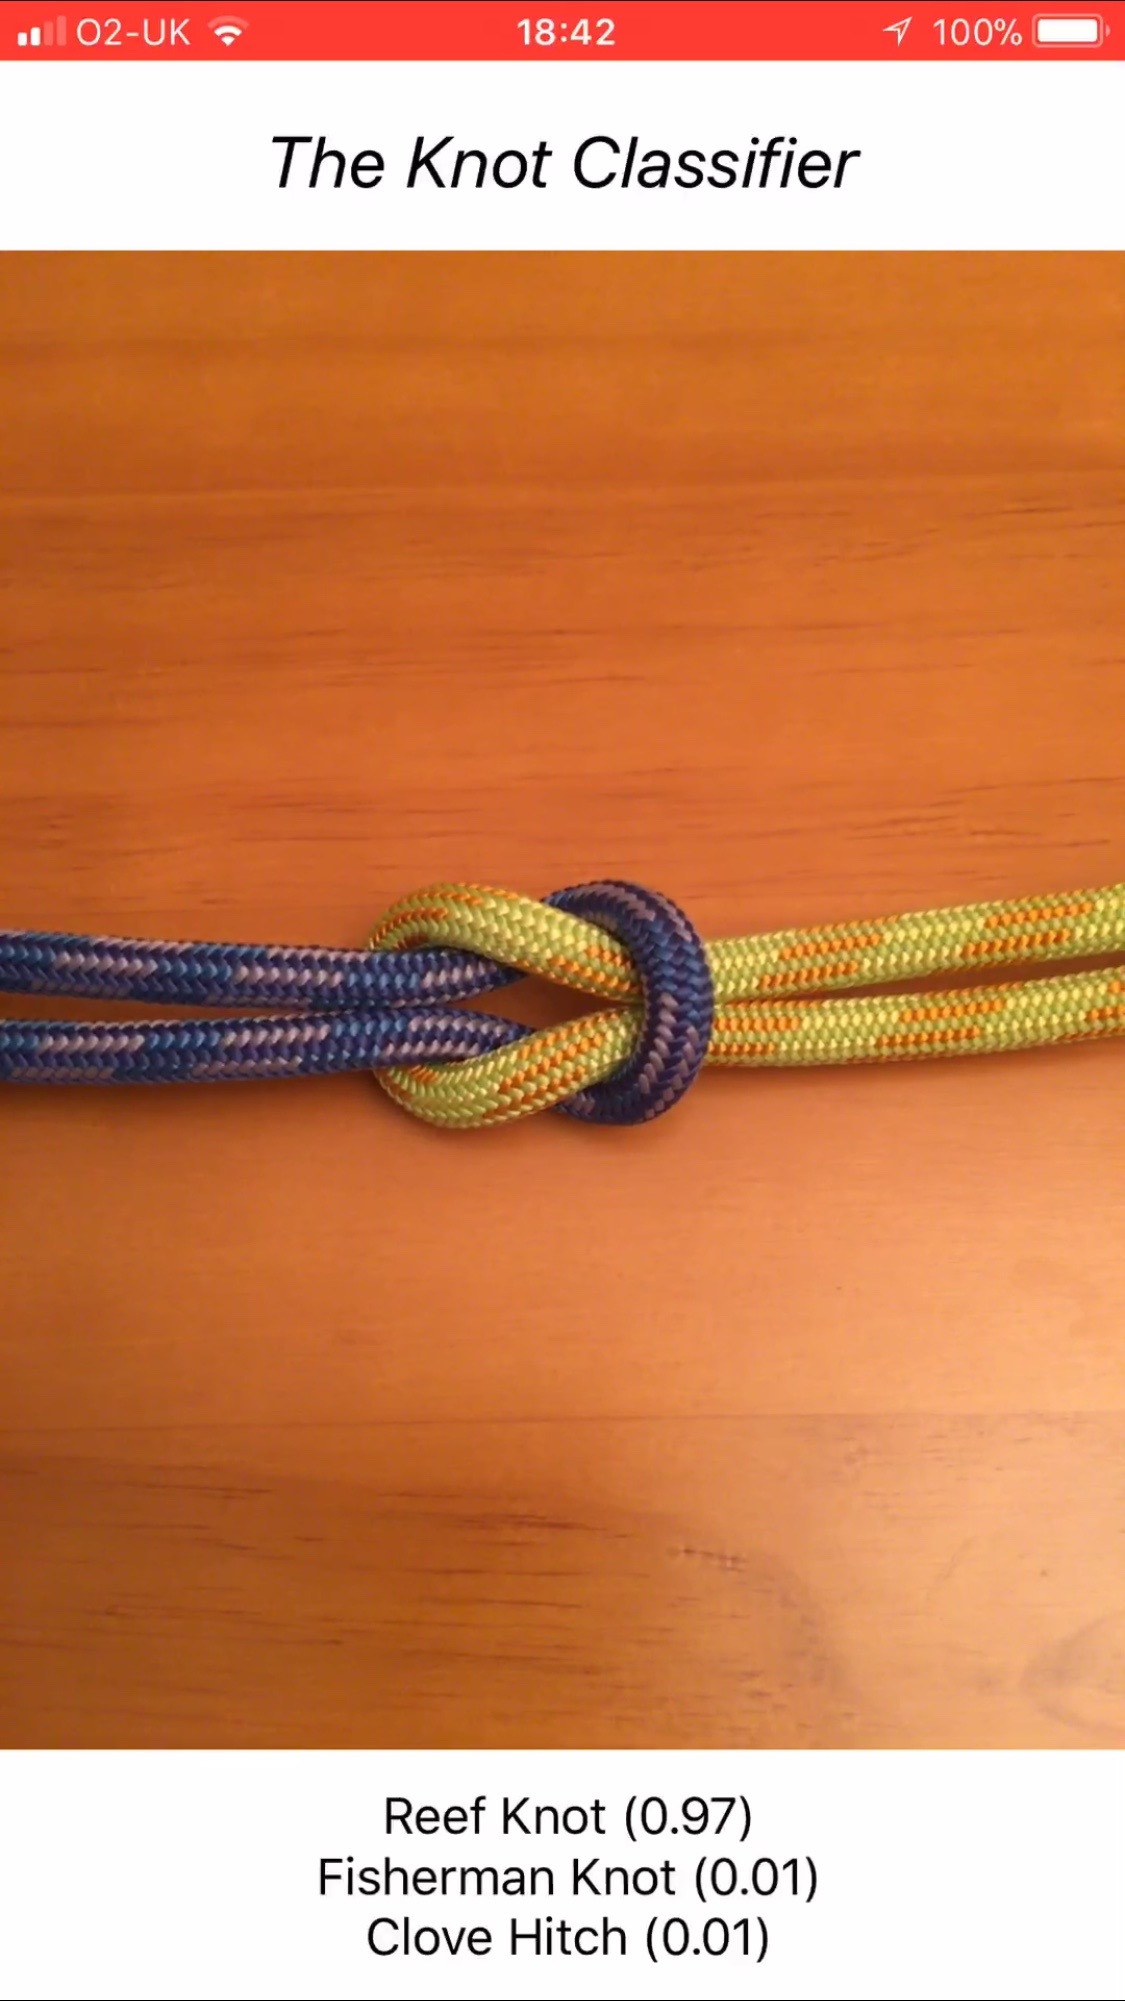
\includegraphics[scale=0.1]{IntroApp}
	\caption{The Final iOS Application Interface}
	\label{fig:IntroApp}
\end{figure}

\section{Scope \& Requirements}
When undertaking a project of this nature, it is critical to craft an appropriate set of requirements and define a realistic project scope.
Due to time constraints and resource constraints, it was important to focus on certain aspects of the project and answering particular questions of high relevance, rather than attempting to discover the answer to every possible related question.
In an effort to keep focus throughout the entire academic year on what I deemed to be important within this project, I self-defined the following requirements and I self-defined the scope of the project.

\subsection{Critical Requirements}
First of all, the main aim of this project is to determine whether or not it is possible to classify knots based solely on their topology from images.
In conjunction with this aim, the first critical requirement of this project is to successfully design and implement a convolutional neural network that is capable of classifying knots.
However, to successfully implement a convolutional neural network, it must first be trained on data.
Furthermore, the convolutional neural network can only be used on or evaluated on data.

Therefore, the second critical requirement of this project is to create a training dataset to train the convolutional neural network and a validation/test dataset to evaluate the performance of the convolutional neural network.
There are thousands upon thousands of knots that could potentially be classified, however, in the best interests of creating high-quality datasets given the time constraint of two semesters, the number of knots to be classified was restricted to ten.
Therefore, the first two critical requirements of this project are to classify ten knots with the use of a convolutional neural network and to create datasets with which to train and evaluate the convolutional neural network.

When crafting these two initial critical requirements, an interesting research question surfaced that would also clarify the scope of this project.
That research question was the following.
What features within a knots dataset or a convolutional neural network model may enhance or alter the knot classification performance of a convolutional neural network?
The scope of this research question must be clearly defined because there is potentially an infinite number of features that may influence classification performance.
Also, the question can be split further into two separate questions:
\begin{itemize}
	\item What features of the dataset will affect knot classification?
	\item What features of the deep learning model will affect knot classification?
\end{itemize}
Therefore, the considered features will be limited to a handful of features that can be found within the datasets and the convolutional neural network model architecture.
Features within the dataset will only be considered if they affect solely the visualisation of the knot topology.
For example, lighting will be considered, because shadows appearing across different knot topologies within photographs may noticeably affect the appearance of a knot.
Also, when attempting to classify a knot out-with controlled, experimental conditions, the lighting may significantly differ.
However, it is not feasible to attempt to measure how different backgrounds may affect classification performance because there an infinite number of backgrounds to measure.
Neural network models can significantly differ, however, the most comprehensive way of measuring a neural network is to measure its size or number of trainable parameters.
The more trainable parameters a neural network has, the bigger it is considered to be.
As a result, the only feature of the models that will be considered is their size, and how their size may affect the classification performance.

The third critical requirement is to implement a convolutional neural network that can robustly classify knots, meaning it can classify knots regardless of brightness or rotation.
This requirement is intrinsically linked with the second critical requirement in the sense that a convolutional neural network must be trained on a dataset containing a variety of different features to discourage the classifier from only recognising one knot orientation for example.
Variables such as knot rotation and image brightness will be considered to fulfil this requirement, but some variables such as rope material cannot be treated in the same way due to resource constraints.
Of course, knots can be tied in a variety of materials but not all possible materials can be summoned for evaluation in this project.
Climbing rope will be used to tie every knot. 

The fourth and final critical requirement of this project is to build a portable interface with which to utilise the knot classification convolutional neural network.
Furthermore, the classification must be instantaneous, minimal and provide different levels of certainty.
Knots are very commonly encountered and used in outdoor environments where no desktop computers or power outlets are reasonably available. Therefore, it is sensible to consider providing a mechanism by which users can utilise the results of this project in such environments.

On a final note with regard to the project's scope, a final research question of interest surfaced.
That research question was the following:
\begin{itemize}
	\item What techniques can prevent the deep learning model from overfitting?
\end{itemize}
When fulfilling the answer to this question the aim is to fully explore techniques that combat the issue of overfitting that can commonly occur in deep learning.
Overfitting is a prevalent issue that can occur when performing image classification, and it will be explained in more detail in the background chapter.
Every dataset used in this project will be minimal in comparison to datasets such as ImageNet \cite{imagenet_cvpr09} that were used to solve previous image classification tasks.
The datasets will be small in size due to time constraints and due to the fact that they will be created from scratch.
Overfitting is a common issue that is encountered when small datasets are used to train and validate neural networks, and so overfitting will likely be a significant hurdle to overcome in this project. 
Therefore techniques such as data augmentation and dropout will be explored to provide insight into how accurate an image classifier can be, even with minimal training and validation data.  

% SUBSECTION
%\subsection{A subsection}

% INCLUDE FIGURE
%%\vspace{-7mm}
%\begin{figure}
%\centering
%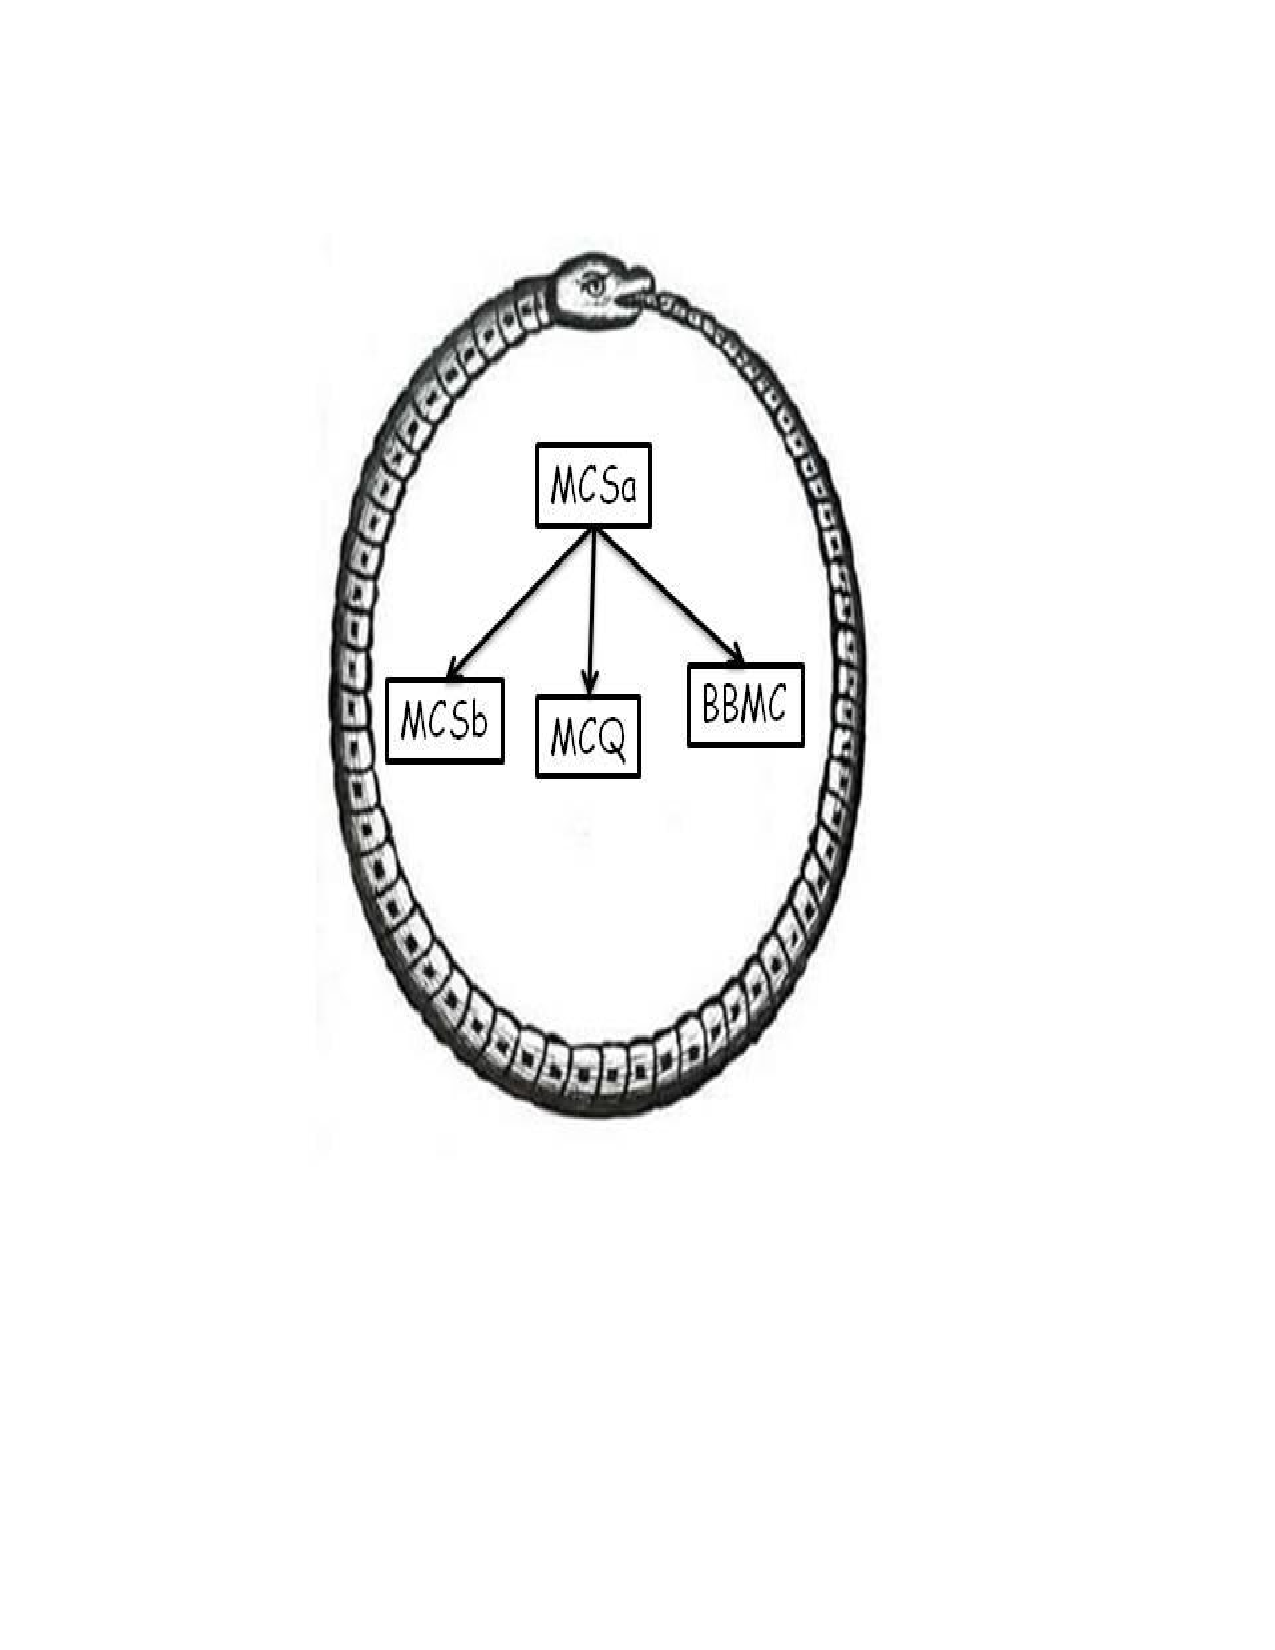
\includegraphics[height=9.2cm,width=13.2cm]{uroboros.pdf}
%\vspace{-30mm}
%\caption{An alternative hierarchy of the algorithms.}
%\label{uroborus}
%\end{figure}

% REFERENCE A FIGURE
%(Figure \ref{uroborus}).

% VERBATIM
%\begin{verbatim}
%
%            > pdflatex example0
%            > bibtex example0
%            > pdflatex example0
%            > pdflatex example0
%
%\end{verbatim}

%---------------------------------------------

% BACKGROUND

\chapter{Background}

After conducting initial thorough research, it became clear that there is no other project in existence that claims to understand knot topology through using machine learning.
Hence, when conducting background research on literature in this field, it was important to seek literature on previous image classification tasks and fundamental machine learning techniques in general.
Throughout this chapter, the project's requirements and scope will be reinforced in conjunction with providing the appropriate background.

\section{Knots}
Firstly, it is important to mention that this project does not investigate mathematical knots.
Instead, this project investigates the topology of knots tied in rope for use in practical applications.
An invaluable resource for researching and gathering information about knots is the Ashley Book of Knots\cite{ashley1947ashley}, and it has been the resource used to select all ten of the knots that will be classified and manipulated in this project.

% Provide a brief history of knots?

Throughout the known world, there are many, many knots. 
There are far more than an individual could ever hope to possibly know and tie with no external information.
In addition to this, there are many categories to which all these knots belong.
Each category is made up of knots with similar properties.
A good example of such a category is the category of bend knots.
Bend knots are used to unite two ropes and have the characteristic to never come undone under tension.
An example of a bend knot is the Fisherman's Knot.

At the other end of the spectrum, there are loop knots that can be used to tie a closed circle in rope.
An example of a loop knot is the Figure-8 Loop.

As mentioned above, there is an astronomically large number of knots.
Therefore, a reasonable, small number of ten knots were selected for use in this project.
However, it was important to best represent the spectrum of all knot categories with these ten knots, in order to obtain more general and conclusive analysis on the learned representation of knot topology.
This means ten knots were strategically picked based on their category.
The ten knots that were used in this project can be seen in Figure \ref{fig:knots} located in Appendix \ref{appendix:Knots}.
A description of each knot follows:
\begin{itemize}
	\item \textbf{The Alpine Butterfly Knot}: The Alpine Butterfly Knot is a loop knot traditionally used in climbing. It is typically used to form loops mid-way along a length of rope. An example of the Alpine Butterfly Knot can be seen in Figure \ref{fig:ABK}.
	\item \textbf{The Bowline Knot}: The Bowline Knot is a loop knot of ancient origin. It is typically used to create a loop at the end of a length of rope. An example of the Bowline Knot can be seen in Figure \ref{fig:Bowline}.
	\item \textbf{The Clove Hitch}: The Clove Hitch is a hitch knot of ancient origin. It is typically used to secure rope around objects such as posts or trees. An example of the Clove Hitch can be seen in Figure \ref{fig:CloveHitch}.
	\item \textbf{The Figure-8 Knot}: The Figure-8 Knot is a stopper knot of ancient origin. It is typically used to prevent rope from slipping through a narrow passage or come undone. An example of the Figure-8 Knot can be seen in Figure \ref{fig:Fig8Knot}.
	\item \textbf{The Figure-8 Loop}: The Figure-8 Loop (specifically, the Figure-8 on a bight) is a loop knot traditionally used in climbing to form a loop in rope that will likely stay tied, even under immense load. An example of the Figure-8 Loop can be seen in Figure \ref{fig:Fig8Loop}.
	\item \textbf{The Fisherman's Knot}: The Fisherman's Knot is a bend knot of ancient origin. It is typically used to unite two separate lengths of rope into one single length of rope. An example of the Fisherman's Knot can be seen in Figure \ref{fig:Fisherman}.
	\item \textbf{The Flemish Bend}: The Flemish Bend is a bend knot of ancient origin. It is typically used to unite two separate lengths of rope into one single length of rope. An example of the Flemish Bend can be seen in Figure \ref{fig:Flemish}.
	\item \textbf{The Overhand Knot}: The Overhand Knot is one of the most fundamental and ancient of all knots. Primarily, it is used as a traditional stopper knot, but can form the basis for many other well-known knot topologies. An example of the Overhand Knot can be seen in Figure \ref{fig:Overhand}.
	\item \textbf{The Reef Knot}: The Reef Knot is a binding knot of ancient origin, although it can also be categorised as a bend knot. It is typically used to unite two separate lengths of rope into one single length of rope, however, it is only recommended to fulfil this purpose if both lengths of rope in question are of equal diameter. An example of the Reef Knot can be seen in Figure \ref{fig:Reef}.
	\item \textbf{The Slip Knot}: The Slip Knot is a stopper knot of ancient origin. It is typically used to prevent rope from slipping through a narrow passage or come undone, however, the slip knot can be quickly untied or 'slipped' by pulling the free end of the rope. An example of the Slip Knot can be seen in Figure \ref{fig:Slip}.
\end{itemize}  

\section{Machine Learning}
Machine learning is the art and science of giving machines the ability to learn without explicit programming.
Such learning relies heavily on data, and furthermore, the representations and patterns within that data. 
However, the ultimate goal of machine learning is to automate problem-solving without human intervention.
For example, this project aims to recognise a knot from an image without explicitly stating what the knot is.
This is a perfect example of the problem known as image classification, which can be solved effectively with machine learning techniques.
However, before further exploring the problem of image classification, it is first important to understand some basic core and relevant principles of machine learning.

\subsection{Supervised \& Unsupervised Learning}

Typically, machine learning techniques involve the employment of a training stage and a validation stage.
The training stage is an opportunity for machine learning algorithms to begin understanding and learning features in training data, where the training data should try to best represent data that will be encountered after training.
During the training stage, the machine learning algorithm crafts what is known as a model to represent patterns found in the data.
The validation stage is an opportunity to evaluate how effective the algorithm's model is at accomplishing a task that it was trained to do during the training stage.
In a similar fashion to the learning process of a human, the training stage of the algorithm is a crucial component of the learning process where feedback is given, and the algorithm improves through practice on the training data.
Each iteration of the training stage is known as an epoch.

In machine learning, there are many ways in which the training data can be presented during the training stage, and this has generally resulted in two broad types of learning within the field. 
These types of learning are known as Supervised Learning and Unsupervised Learning. 
In supervised learning, training data is labelled and known, meaning the algorithm can evaluate itself against the data. 
In unsupervised learning, training data is not labelled, hence the algorithm is left to find its own representation of the data.
Only supervised learning will be used within the scope of this project. 

\subsection{Classification}
Classification is the term used to describe the process of categorising new observations into classes.
Binary classification is the process of deciding whether an object is x or y, while multi-class classification is the process of categorising observations into three or more classes.
When classifying data, it is first important to understand the representation of the data.
Data can typically be represented as a point on a 2D graph, for the purposes of classification.
Mathematically, it is possible to identify which category an object belongs to, if there is training data present to indicate where on the graph that category commonly appears.
If new data appears in the same region as a certain category, we can predict that new data to be an object of that specific category.
The model, which was created by a specified machine learning algorithm, can be represented by a linear or non-linear function that forms a boundary between various categories. 
It is this boundary model that we wish to obtain from classification algorithms.
When fitting a model to training data, a useful metric of the model's performance is its loss, which is defined as the average distance of the model from all of the collective data points on the graph.
A model's loss can reveal how closely the model has fit to either training or test data.

\subsection{Deep Learning}
Deep Learning is a broad subfield of machine learning in which a computational model known as a neural network is used to create models and hence solve problems.
Neural networks are heavily based on the process the biological brain uses to solve problems. 
Recently, deep learning has been able to overcome the massive issue of feature extraction that occurs in traditional machine learning.
In traditional machine learning approaches, a programmer must explicitly explain what features the algorithm should look out for.
On the other hand, deep learning can overcome and circumvent this issue, as neural networks are extremely adept at automatically identifying important features.
As a result, deep learning has provided more promising results in almost every domain when compared to traditional machine learning techniques.
Hence, deep learning has quickly become a potent and popular tool in the machine learning toolkit.

\subsubsection{Neural Networks}
A neural network is made up of neurons.
The neuron is the fundamental unit of any neural network.
A neuron accepts a set of weighted inputs and then outputs a value in correspondence to a specific function.
There are many types of neuron, for example, the sigmoidal neuron outputs a value between 0 and 1, although the concept described above is prevalent in all types of neuron.
A neural network begins to arise when these neurons are connected together, to input data, and a specific construct for the output.
The output could be any data type or data structure.
Layers of neurons between the input and output layers are commonly referred to as hidden layers.

In order to simplify and mimic the structure of neurons in the biological brain, neurons within a neural network are typically organised into layers.
When organised in layers, neurons are only connected to neurons in another layer; they are not connected to neurons in their same layer.
Neural networks that have one direction of information flow, where the output of one layer is connected to the input of another layer, are known as feed-forward neural networks because information only propagates in one direction which is forwards.
Conversely, neural networks that propagate information in both the forwards and backwards directions are known as recursive neural networks.
However, only feed-forward neural networks will be considered within this project.

\subsection{Machine Learning Problems}
Unfortunately, machine learning does not routinely deliver perfect results for every problem.
Sometimes, when given training data and validation data, a model may perfectly conform to predict the training data it has been trained on, but consistently predict new test data incorrectly. 
This occurs because the model has fit to the training data so well, that it deviates massively from the possible placement of new and unknown data points. 
This means the model may incorrectly classify or predict any significantly different data in comparison to the training data. 
This phenomenon is known as overfitting and is a common challenge to overcome when performing image classification, particularly if using a small dataset.
An example of what an overfitting model may look like in comparison to a generalised model in the context of performing classification is shown in Figure \ref{fig:BackgroundOverfitting}.

\begin{figure}[h]
	\centering
	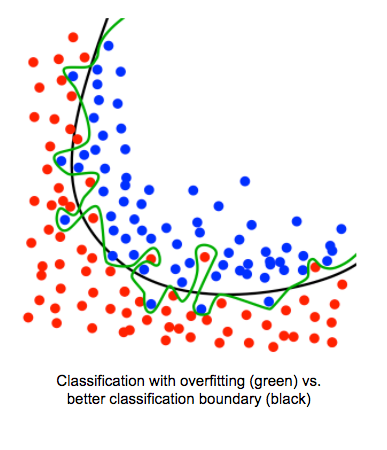
\includegraphics[scale=0.5]{classification-with-overfitting}
	\caption{A Visual Example of Overfitting. Figure from \cite{overfittingGraph}.}
	\label{fig:BackgroundOverfitting}
\end{figure}

Conversely, a model may generalise to multiple training data points very well, but not conform to important small details, causing a decrease in performance.
This phenomenon is known as underfitting.
Within the scope of this project, overfitting is likely to occur when attempting to perform image classification.


\section{Image Classification}
A sub-problem of classification is image classification, where new observations are images, and the goal is to identify which category objects within an image belong to.
Put simply; image classification is the process of identifying objects within images and assigning a representation, such as a class label, to those recognised objects.
As mentioned previously, a major goal of this project is to classify knots within images.
The best way of achieving this goal is to perform image classification.
Image classification can be achieved through a variety of techniques.
The first approaches towards achieving basic image classification were possible through the use of support vector machine algorithms and nearest-neighbour algorithms.
However, the use of neural networks within deep learning has yielded the most promising results in image classification problems.
In fact, there is a type of neural network known as the convolutional neural network that is tailored for image classification and vision problems in general.
In 2012, Alex Krizhevsky, Ilya Sutskever and Geoffrey E. Hinton authored and released their paper entitled "ImageNet Classification with Deep Convolutional Networks" \cite{Krizhevsky:2012:ICD:2999134.2999257}.
This paper lays out many state-of-the-art principles used to achieve image classification, with one of the main principles being the use of a convolutional neural network.
The classification framework and convolutional neural network Krizhevsky et al. used also incorporated techniques such as data augmentation and dropout to combat overfitting.
These techniques will be discussed in further detail later in this chapter.
Similarly, Karen Simonyan and Andrew Zisserman released a paper entitled "Very Deep Convolutional Networks For Large-Scale Image Recognition", in which a convolutional neural network is also used to perform image classification \cite{DBLP:journals/corr/SimonyanZ14a}.

These papers demonstrated that a deep learning approach to image classification through the use of convolutional neural networks can provide state-of-the-art results.
So, it was quickly decided that a convolutional neural network would be the construct of choice for performing image classification in this project.

\subsection{Convolutional Neural Networks}
Convolutional neural networks are deep neural networks that analyse visual imagery.
Convolutional neural networks do this by applying convolutional operations.
Fundamentally, a convolutional neural network consists of an input layer, an output layer and multiple hidden layers in between.
The hidden layers can be fully-connected layers, convolutional layers, activation layers, pooling layers and normalisation layers.
Convolutional neural networks are heavily inspired by biological visual systems found in organisms.
Fully connected layers are layers where each neuron has connections to every activation in the previous layer.
Convolutional layers are layers where convolutional operations are applied to images.
Convolutional operations involve the use of a filter to produce an output average value from each channel of pixel values in an image.
An RGB colour image has three channels, one for red, one for green and one for blue.
Activation layers are responsible for creating an activation map from the output of the convolutional layer.
This is typically achieved using an activation function such as the ReLU activation function \cite{Nair:2010:RLU:3104322.3104425}. 
Pooling layers are then used to perform downsampling operations and reduce the spacial size on the activation map which is the output of the activation layers.
This reduces overall computation and combats overfitting.
Finally, normalisation layers are used to normalise data, meaning that the data will have a mean of zero and a standard deviation of one.
Normalisation such as batch normalisation\cite{Ioffe:2015:BNA:3045118.3045167} can potentially increase a neural network's performance and stability by accelerating the training period.

A convolutional neural network is commonly organised into convolutional blocks, consisting of convolutional layers, activation layers, pooling layers and possibly normalisation layers in that order. 
Fully-connected layers followed by an activation function will then commonly appear at the end of the network architecture in order to correctly format the output.
For multi-class classification tasks, the final activation function used must be a softmax activation function in order to produce an array of values between 0 and 1.

\section{Combatting Overfitting}
In order to overcome the problems with machine learning that are mentioned earlier in this chapter, there are many specific techniques that can be employed.
Typically, when dealing with a small dataset, like the one that will be created for this project, overfitting is generally the biggest problem faced.
Neural networks can contain many hidden layers between the input and output layers, making them extremely complex models that can learn many deep relationships in data.
However, when using a small dataset, this precise learning ability may result in a neural network learning noise from and specific to the training dataset that does not necessarily represent data from the real world.
If this occurs, the neural network will almost certainly successfully learn representations within the training data, but it will consistently fail to correctly predict or classify test data, thus rendering the model effectively useful to only one set of data.
Concerning neural networks, a big contributing factor to overfitting is the number of training parameters available to train.
The more parameters, or weights, that can be trained, the lower the loss will be on training data, but this may result in a model that wildly mispredicts test data.

Unfortunately, due to these reasons, the problem of overfitting continues to appear in deep learning.
Therefore, various techniques have been discovered, designed and employed to combat overfitting. 
Throughout the project's implementation, these many techniques to combat overfitting will be used and the aim of this section is to provide the appropriate background knowledge of these techniques.

\subsection{Data Augmentation}
Data augmentation is a common technique used to combat overfitting.
Although, data augmentation is a technique that does not interfere with the model directly.
Instead, this technique is applied to the dataset that is used to train a model \cite{Simard:2003:BPC:938980.939477}.
As mentioned previously, overfitting can occur when a model only learns representations that specifically apply to the training dataset.
The idea of data augmentation is to expand the dataset, and produce new and slightly-altered data so that a model can learn a broader representation that may apply to real-world data and thus, reduce overfitting.
Hence, data augmentation aims to eliminate the problem of a model learning too few representations.
Simple data augmentation parameters include rotating images and adjusting the zoom scale of images.

Overall, data augmentation can expand the representation of data, thus allowing a small dataset to be transformed into a broader, more representative dataset of the real-world.
Data augmentation can allow a model to better generalise and combat overfitting very effectively \cite{Perez2017TheEO}.

\subsection{Dropout}
Dropout is a technique designed to combat overfitting that was introduced by Srivastava et al. \cite{Srivastava:2014:DSW:2627435.2670313} in 2014.
Specifically, dropout is a form of regularisation used to combat overfitting that may occur in neural networks used in deep learning.
Furthermore, within this paper, dropout was shown to significantly reduce overfitting in comparison to many other regularisation methods such as L1 and L2 regularisation \cite{Ng:2004:FSL:1015330.1015435}.
Essentially, dropout is the process of disabling a certain number, or percentage, of neurons within a specified hidden or visible layer.
For example, if a dropout of 50\% is specified for a certain hidden layer, that means that 50\% of all neurons in that layer will be disabled, including the connections stemming to and from those neurons. 
It must be noted that the disabled neurons are selected randomly.
Also, dropout is only applied during the training stage, not during the validation or prediction stages.

Dropout combats overfitting because it prevents the individual neurons within a neural network from learning together all at once as a dependent group.
Rather, each neuron is then forced to learn multiple features within the data on its own.
This results in a stronger learned representation overall, and the network will less likely overfit.  

\section{Evaluating Machine Learning Models}

\subsection{t-SNE Visualisation}
t-SNE stands for t-distributed stochastic neighbour embedding, and it is a machine learning algorithm that was developed by Laurens van der Maaten and Geoffrey Hinton \cite{vanDerMaaten2008}.
The purpose of t-SNE is to perform dimensionality reduction on data.
This is an instrumental visualisation technique in machine learning because high-dimensional data can be embedded into a space of two or three dimensions, meaning data and all of its clusters or patterns can be visualised and analysed.
This level of visualisation can uncover many high-level representations that have been learned by a neural network.

\subsection{Training History}
The training history of a model can uncover a lot about a model's behaviour.
The training history of a model refers to the training accuracy, the validation accuracy, the training loss and the validation loss.
The training accuracy is the accuracy of the model when predicting or classifying the training data.
The validation accuracy is the accuracy of the model when predicting or classifying the validation data.
The training loss is the loss of the model when it is fit to the training data.
The validation loss is the loss of the model when it is fit to the validation data.
If a model's accuracy at predicting training and validation data has been recorded for every epoch of training, along with the model's loss when fit to training and validation data for every epoch of training, that information can be useful in uncovering whether the model has overfit to the training data or underfit to the training data.
Clear signs of overfitting or underfitting can be uncovered by a model's training history.
For example, if the training accuracy is high and the training loss is low, but the validation accuracy is low and the validation loss is high, this is a clear sign that the validation data is too far from the representation of the training data, and hence, overfitting has occurred.
For this reason, it is essential to always keep a record of a model's training history for further analysis.

\subsection{Confusion Matrix Plots}
For classification tasks, a common and acceptable measure of classification performance can be visualised by a confusion matrix plot.
A confusion matrix simply presents the predicted class labels given to test data by a classifier compared to the true class labels of the test data.
The y-axis for a confusion matrix represents the true labels of the test data being given to the classifier that is being evaluated, and the x-axis represents predicted labels given to the test data by the classifier that is being evaluated.
Hence, a perfect classifier would create a perfect diagonal in a confusion matrix.
Confusion matrices can be extremely useful in analysing classification performance because they can highlight what classes are being misclassified, and what the predicted classes actually are for the misclassified data, meaning that useful patterns and trends may be noticed within the classifier.

%---------------------------------------------

% DESIGN

\chapter{Design}
This chapter details the design processes for the datasets, the knot classification framework and the classifier's interface.

\section{Dataset Design}
Every machine learning task begins with data.
In order to classify knots from images, a dataset containing many images of these knots must be created.
The dataset shall consist of training data and validation data, and a convolutional neural network will be trained on the training data and validated on the validation data.
The dataset will combine two types of data, controlled data and wild data.
The controlled data shall be created from scratch for the sole purpose of this project.
The wild data shall be found from online sources and should be completely independent in comparison to the controlled data, in order to provide a fair evaluation of the classifier's true capabilities.
After creating the controlled and wild datasets, the entire dataset will then be formed with a combination of the controlled and wild datasets, where the training and validation datasets will emerge following an 80\% : 20\% split on the entire dataset.
It is recommended to split the entire data in this way to obtain the training and validation datasets, but there is no optimal ratio for splitting the dataset into train and validation datasets.

\subsection{The Controlled Dataset}
When considering what features the knot classifier should overcome, the dataset was designed accordingly.
For example, the knot classifier should be able to classify knots regardless of their rotation or orientation of tying, the image lighting, or the knots' tension.
To achieve this, data of each knot will be taken at 4 different angles along the z-axis, in three different forms of lighting and three tensions.
When being photographed, each knot shall be rotated for every 90 degrees along the z-axis.
They shall be rotated along the z-axis because the 2D planar rotation (in the x and y-axes) can be solved via data augmentation that shall be discussed later.
Every knot shall also be photographed in three different lighting conditions.
The three lighting conditions shall be diffuse light, meaning normal daytime light, directed source light from one side and directed source light from immediately above the knot.
The lighting is considered in order to thoroughly investigate whether certain shadows in the images affect the classification results.
Also, it is used as a measure to prevent the classifier from succumbing to different lighting conditions.
Finally, every knot will be captured at a set tension or as it would appear when correctly tied, at a loose tension, and finally at an extremely loose tension or to the point of almost coming undone.
Similarly to the reasons for capturing knots in different lighting conditions, this is done to later investigate whether tension affects the classification performance and this is also done to prevent the final classifier from failing to classify knots that have been loosely tied or vice versa.
A final factor that must be taken into account is the background of each knot image.
It will be interesting to explore how background may alter the classification performance. 
Therefore, one entire dataset as described above will be taken with a slightly reflective background, and another dataset as described above will be taken with a plain non-reflective background.

Considering these variables within the dataset, it is expected that each knot class will be represented by 144 images, leading to a total of 1440 images for the entire controlled dataset.

\subsection{The Wild Dataset}
In order to fairly evaluate the trained classifier, it is important to consider using validation data that the classifier will likely encounter in the real world, but not data that the classifier has already been trained on.
Hence, this data must be somewhat foreign and different when compared to the controlled dataset that is used for training.
This foreign data is referred to as wild data throughout this project.
Of course, every image within this wild dataset must contain correct and accurate photos of each knot, but they must originate from a different source to avoid any unwanted bias.
To successfully do this, it was decided that the images would be collected from a specific few resources on the internet.
These specified resources are Google Images, Flickr and ImageNet.
Furthermore, it was planned to try and collect 20 images per knot class, leading to a total of 200 images for the wild dataset.

\section{Classification Framework}
A major goal of this project is to classify knots based on type from images.
Therefore, it was quickly decided that a deep convolutional neural network would be used to produce a class index within an array which corresponds to one of the ten specified knot classes.
Furthermore, for the purposes of exploring what features of the model architecture affect classification performance, three convolutional neural network architectures were designed. 
These three model architectures are the small model architecture, the medium model architecture and the large model architecture, where the only difference between the three models is the number of training parameters.
This was done in order to later examine the impact that the number of training parameters would have on the overall classification performance.

When previously considering the design of the training and validation datasets, it became clear that the convolutional neural networks must be designed in such a way that they combat the problem of overfitting that may arise from the size and contents of the datasets.
Due to time constraints, the datasets may contain approximately 1640 images in total, which is certainly very small in comparison to other image classification tasks, such as those that involve ImageNet, which is a well-known dataset containing upwards of 3 million images \cite{imagenet_cvpr09}.
Also, due to time constraints, the datasets, particularly the controlled dataset, may contain content that is quite repetitive.
For example, it was planned that only two types of climbing rope are to be used in the controlled datasets.
These two factors significantly increase the chances of overfitting, and so any considered convolutional neural networks were designed to incorporate data augmentation and dropout.

\subsection{Data Augmentation}
Due to a small dataset, data augmentation is a crucial technique that shall be employed to prevent overfitting in this knot classifier.
When deciding which features to augment, it was first important to consider the features that the classifier should be robust towards.
A key observation of knots in everyday life is that they can appear in many different forms, and they can be tied in many rotations, but they are still fundamentally the same type of knot.
In other words, a knot classifier should be able to correctly classify a knot no matter what rotation that knot has been tied at.
This ideology can be applied to many other features of knots that the classifier should be robust towards, and it is these considerations that prompted the design of what data augmentation parameters to choose.

As already mentioned, the datasets will contain photos of knots tied at only one orientation.
Hence, it was necessary to design the rotation range of augmented images to equal 360 degrees, therefore promoting the classifier to train on images of knots at every possible rotation.

Another parameter to be considered for augmentation is the zoom range of the knots.
If a dataset contains images of knots taken from only one specific distance or 'zoom' distance, it may be easy for the network to learn features of a knot dependent on that specific zoom and disregard the underlying knot topology.
To combat this, it was decided to consider a form of zoom range augmentation on the images, to therefore promote the knot classifier to correctly classify knots that might be photographed at different distances from that of the dataset's images.

The third important parameter to consider for data augmentation was the orientation of the knots.
It is in fact true that changing the orientation of a knot may change the type of a knot itself, but when considering the ten knots that will be classified in this project, this was not the case.
In fact, every one of the ten knots could be tied at a different orientation, both vertically and horizontally, and still represent the same knot.
Once again, to enforce the real-world robustness of the classifier, it was necessary to consider an implementation design where augmented images could be flipped both horizontally and vertically to ensure that the classifier may still correctly classify knots tied at different orientations from which they may appear in the datasets.

\subsection{Dropout}
Due to the repetitive nature of the controlled dataset, it became apparent that a model may consistently fit the specific representation of the training data rather than learning the general knot topology that is common amongst of possible test data.
Therefore, it was decided to add significant dropout of approximately 50\% to the design of the convolutional neural networks.
It is hoped that the addition of this dropout throughout the network will assist the model to generalise to training and test data rather than solely overfitting to training data. 

\section{The Knot Classifier Smartphone Application}
Another goal of this project is to create a usable and useful interface through which users can utilise the classification convolutional neural network.
In the context of this project, knots are typically used outdoors, where there are typically no accessible desktop computers.
Therefore, it became immediately clear that an application usable on a portable device such as a smartphone was the best solution.

When designing the app, it was particularly important to consider how the trained convolutional neural network would be imported and used in the application.
Concerning the use of the convolutional neural network, there were two avenues to consider.
These avenues were real-time classification and offline classification.
Real-time classification is the term used to define the immediate gain of prediction class labels as soon as data has been observed.
Offline classification is the term used to define the gain of prediction class labels from data that has been previously captured and stored.
In order to decide which of these two paradigms to pursue, it was essential to reconsider the requirements of the application and its interface that were self-defined earlier in this dissertation.
The first requirement of the interface is that it must provide a clear prediction in potentially desolate locations, such as the outdoors which is where users are likely to deal with knots.
With the design of a mobile application, this requirement is satisfied.
The second requirement of the interface is that it must provide instantaneous predictions with minimal interface prompts. 
In pursuit of satisfying this second requirement, it became clear that real-time knot classification became one of the primary goals of the app itself.
When a user is attempting to classify knots while engrossed in particular situations such as climbing, it is far more beneficial and far safer to allow the user to classify the knot in real-time rather than to prompt the user to take a photo and then select the photo from their camera roll.
While it is useful to be able to classify previous photos from a device's camera roll, this is considered to be a secondary goal of the application.
Therefore, the mobile application was designed to perform real-time knot classification where the opening page of the application accesses a device's camera, dependent on privacy settings, and uses the real-time images captured by the device's camera to act as continuous input to the imported knot classification convolutional network. 
Then the convolutional neural network can output the top-3 predicted class labels to the screen clearly to predict exactly what the camera sees in real-time, thus portraying the effect of real-time knot classification.
An example of the initial wireframe design for the application can be seen in Figure \ref{fig:AppDesign}.

\begin{figure}
	\centering
	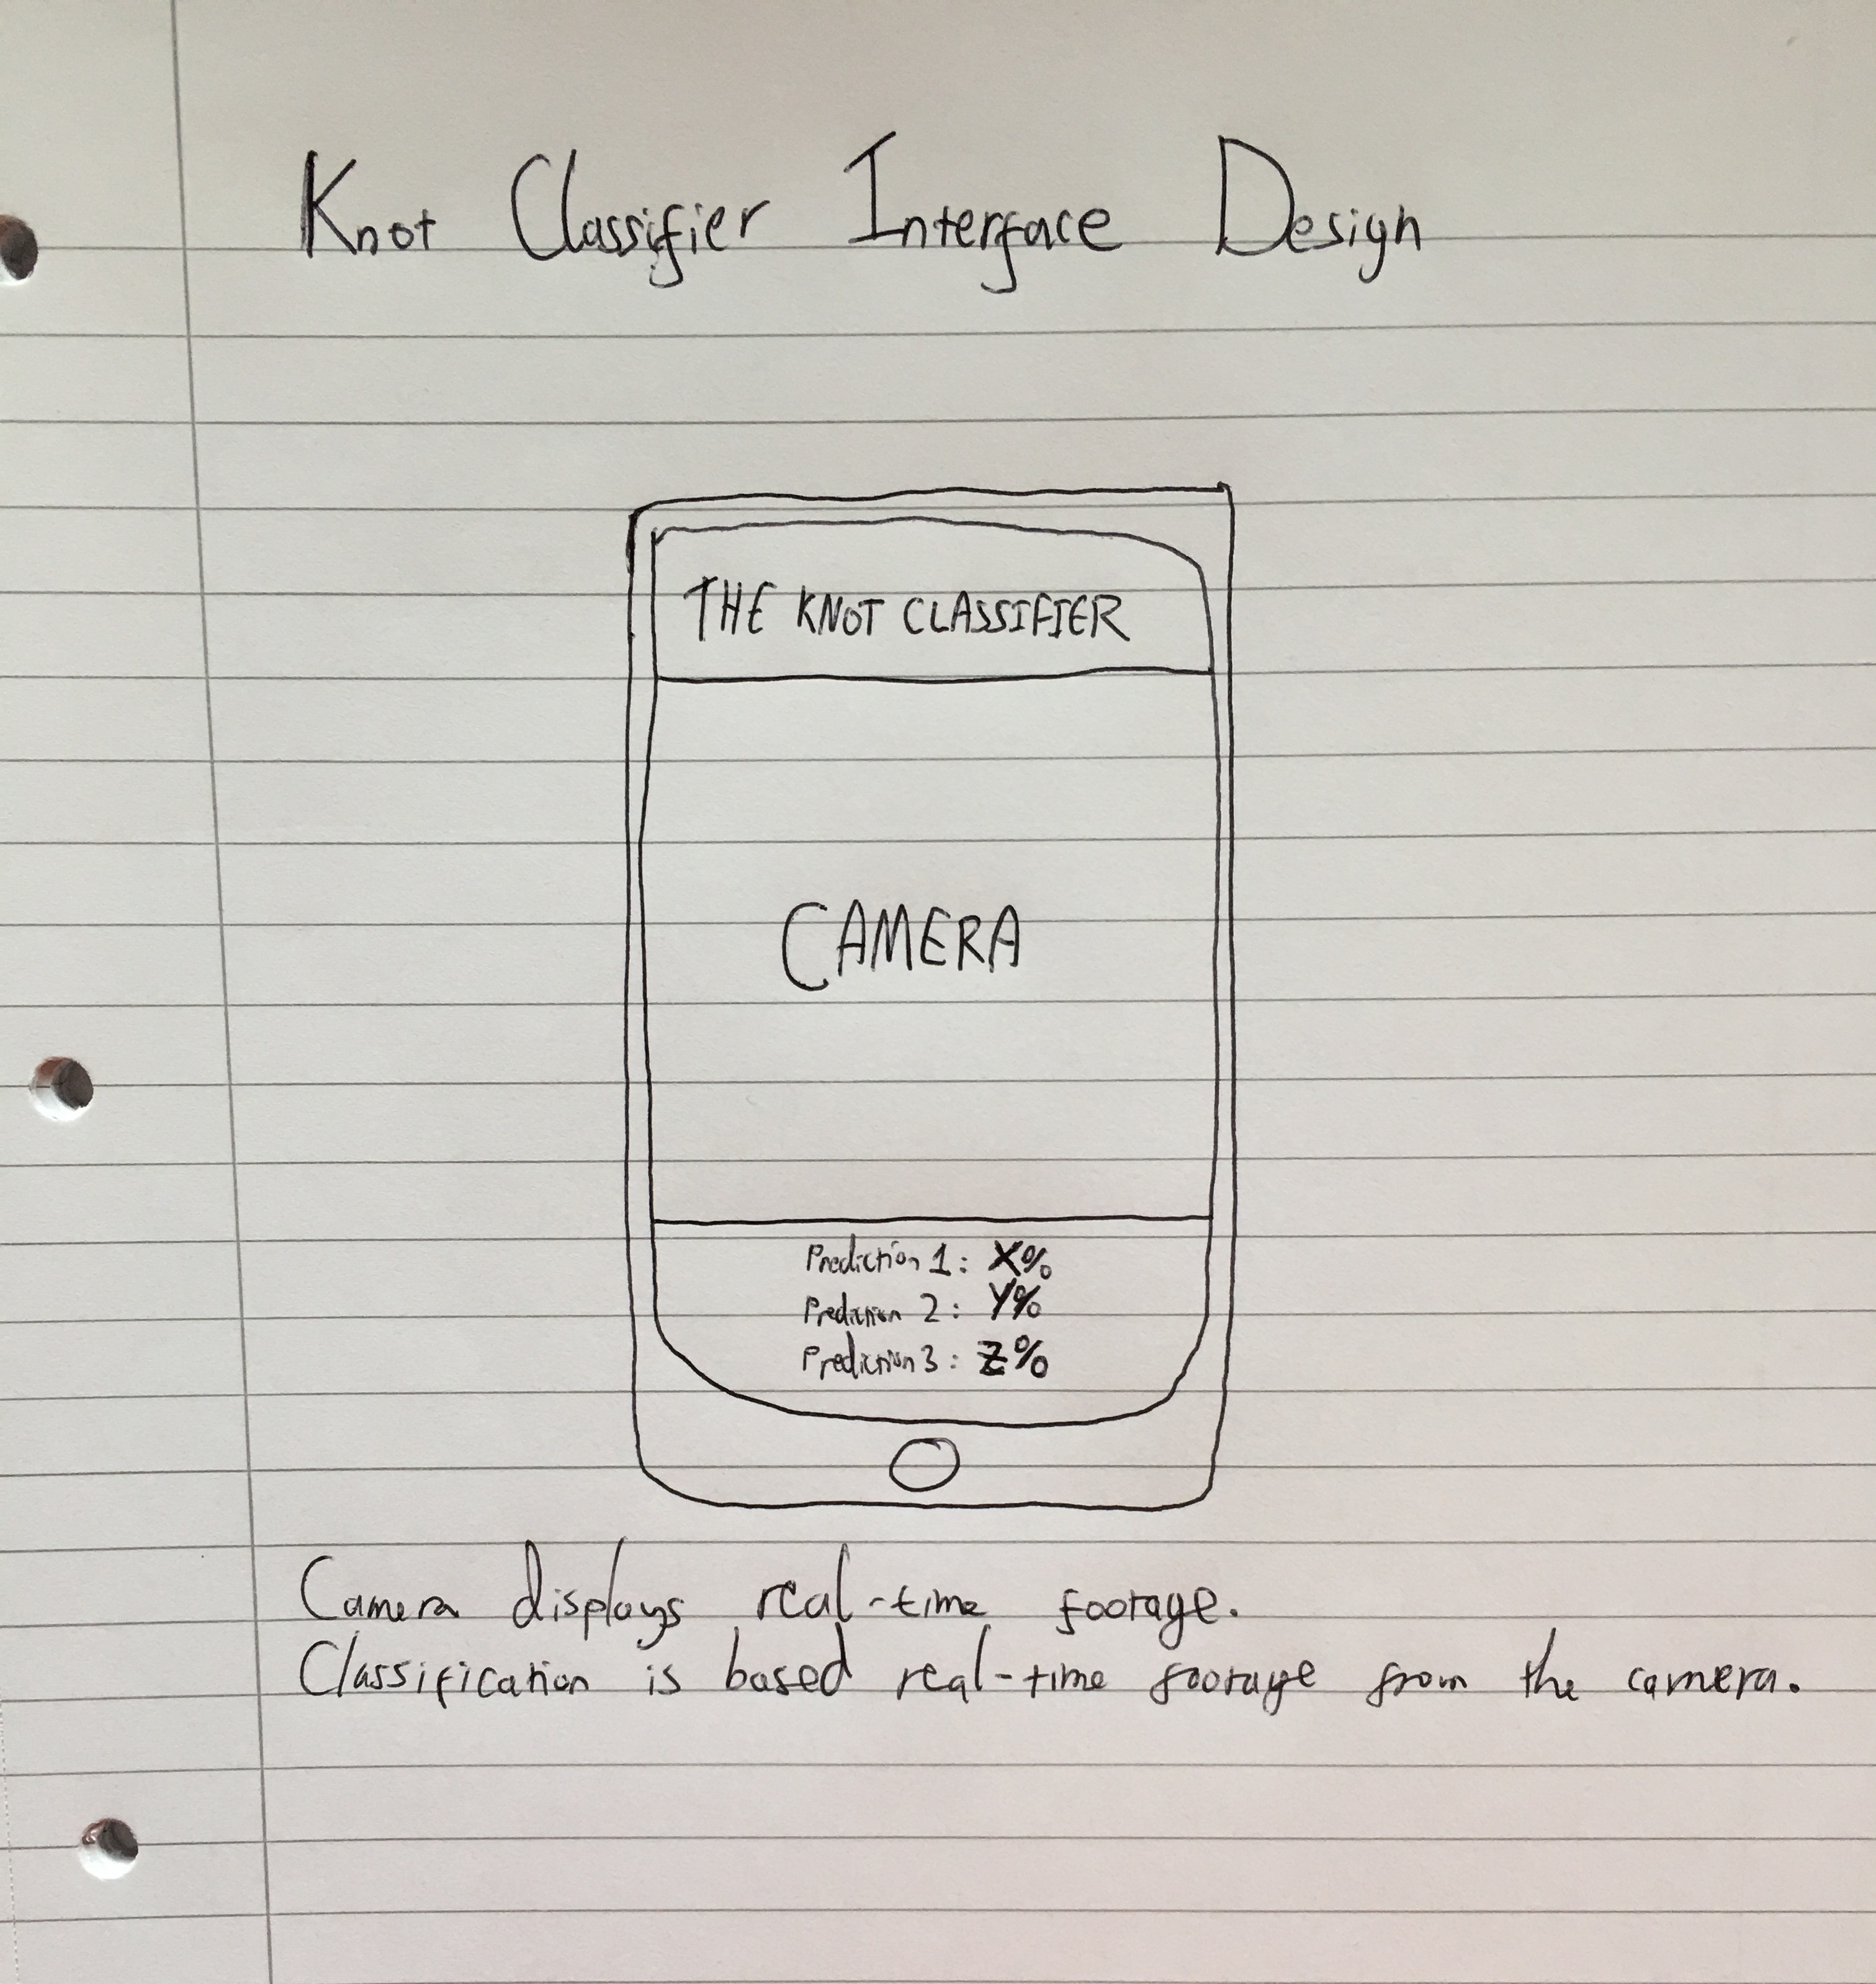
\includegraphics[scale=0.1]{AppDesign}
	\caption{An Initial Wireframe Design of the Mobile Application}
	\label{fig:AppDesign}
\end{figure}

The third requirement of the interface/application is to provide a level of certainty along with the prediction, so as not to confuse the user or mislead the user.
In order to satisfy this requirement, a certainty percentage or probability will be provided along with the predicted class label, as seen in Figure \ref{fig:AppDesign}.
This is a crucial component of the application's usability, as it must be considered that the application will not always correctly predict the knot.
Therefore, even when the prediction is incorrect, the application can still convey a level of certainty about its predictions, and even provide the class labels of the next predictions along with their respective certainties, to give the user alternative predictions and a broader overall prediction other than the top prediction on its own.   

%---------------------------------------------

% IMPLEMENTATION

\chapter{Implementation}
This chapter describes the implementation of:
\begin{itemize}
	\item The knotClassifier.py script. This is a Python script that trains convolutional neural networks.
	\item The ResizeDataset.py script. This is a Python script that resizes .jpg and .png images within a dataset.
	\item The convertModel.py script. This is a Python script that converts Keras HDF5 models to Core ML models.
	\item The Knot Classifier iOS Application.
	\item The datasets that were used to train and validate the knot classifier.
\end{itemize}

\section{Dataset Implementation}
As mentioned previously in the design chapter, every machine learning task begins with data.
In order to correctly classify ten knot topologies, the convolutional neural networks must be trained on a dataset containing an acceptable number of images for every knot.
Hence, both a controlled and a wild dataset containing many images of knots had to be created.
Furthermore, the datasets had to be appropriate to successfully perform this image classification task.

\subsection{Controlled Dataset Creation}
Firstly, the images of the dataset were taken with one camera, the Canon EOS 650D.
Photographs were captured while holding the camera in order to best try and capture the knots themselves at the centre of every photograph.
A tripod was not used because the physical size of every knot differed, and so the detail of knots captured would have differed thus introducing unwanted bias, even if it was small.

Secondly, different lighting conditions as described in the design chapter were simulated with the use of a desk lamp.
The desk lamp's position dictated the lighting conditions for the images. 
The lamp was positioned just out of frame on the right-hand side of every photo for side-lit photos and the lamp was positioned just above the camera lens for directly-lit photos. 
An example of how these different lighting conditions affect photos of the Reef Knot from within the dataset can be seen in Figure \ref{fig:DatasetLighting}.

\begin{figure}[h]
	\begin{subfigure}{.3\textwidth}
		\centering
        \includegraphics[width=\linewidth]{ReefDiffuse}
        \caption{Diffuse Lighting}
        \label{fig:DatasetLightDiffuse}
	\end{subfigure}
	\begin{subfigure}{.3\textwidth}
		\centering
        \includegraphics[width=\linewidth]{ReefSourceSide}
        \caption{Source Lighting from Side}
        \label{fig:DatasetLightSide}
	\end{subfigure}
	\begin{subfigure}{.3\textwidth}
		\centering
        \includegraphics[width=\linewidth]{ReefSourceAbove}
        \caption{Source Lighting from Above}
        \label{fig:DatasetLightAbove}
	\end{subfigure}
	\caption{Lighting Conditions Within Controlled Datasets}
    \label{fig:DatasetLighting}
\end{figure}

Thirdly, every knot, for every lighting condition, was tied at three different tensions as described in the design chapter.
An example of how these different knot tensions affect photos of the Reef Knot from within the dataset can be seen in Figure \ref{fig:DatasetTension}.

\begin{figure}[h]
	\begin{subfigure}{.3\textwidth}
		\centering
        \includegraphics[width=\linewidth]{ReefSet}
        \caption{Set Tension}
        \label{fig:DatasetTensionSet}
	\end{subfigure}
	\begin{subfigure}{.3\textwidth}
		\centering
        \includegraphics[width=\linewidth]{ReefLoose}
        \caption{Loose Tension}
        \label{fig:DatasetTensionLoose}
	\end{subfigure}
	\begin{subfigure}{.3\textwidth}
		\centering
        \includegraphics[width=\linewidth]{ReefVeryLoose}
        \caption{Very Loose Tension}
        \label{fig:DatasetTensionVeryLoose}
	\end{subfigure}
	\caption{Knot Tensions Within Controlled Datasets}
    \label{fig:DatasetTension}
\end{figure}

Lastly, every knot, for every lighting condition and tension, was rotated and photographed for every 90 degrees in the z-axis.
An example of how these different knot rotations affect photos of the Reef Knot from within the dataset can be seen in Figure \ref{fig:DatasetZAxisRotation}.

\begin{figure}[h]
	\begin{subfigure}{.5\textwidth}
		\centering
        \includegraphics[width=.7\linewidth]{Reef0}
        \caption{0 Degrees}
        \label{fig:ZAxisRotation0}
	\end{subfigure}
	\begin{subfigure}{.5\textwidth}
		\centering
        \includegraphics[width=.7\linewidth]{Reef90}
        \caption{90 Degrees}
        \label{fig:ZAxisRotation90}
	\end{subfigure}
	\begin{subfigure}{.5\textwidth}
		\centering
        \includegraphics[width=.7\linewidth]{Reef180}
        \caption{180 Degrees}
        \label{fig:ZAxisRotation180}
	\end{subfigure}
	\begin{subfigure}{.5\textwidth}
		\centering
        \includegraphics[width=.7\linewidth]{Reef270}
        \caption{270 Degrees}
        \label{fig:ZAxisRotation270}
	\end{subfigure}
	\caption{Z-Axis Rotations Within Controlled Datasets}
    \label{fig:DatasetZAxisRotation}
\end{figure}

The last thing to mention in terms of creating the dataset is the background used in the dataset. 
As mentioned in the Design chapter, each dataset was taken with two backgrounds, one reflective background and one non-reflective background.
An example of how these different backgrounds affect photos of the Reef Knot from within the dataset can be seen in Figure \ref{fig:DatasetBackground}.

\begin{figure}[h]
	\begin{subfigure}{.5\textwidth}
		\centering
        \includegraphics[width=.7\linewidth]{ReefReflect}
        \caption{Reflective Background Within Controlled Dataset}
        \label{fig:DatasetReflectBackground}
	\end{subfigure}
	\begin{subfigure}{.5\textwidth}
		\centering
        \includegraphics[width=.7\linewidth]{ReefNoReflect}
        \caption{Non-Reflective Background Within Controlled Dataset}
        \label{fig:DatasetNoReflectBackground}
	\end{subfigure}
	\caption{Backgrounds Within Controlled Dataset}
    \label{fig:DatasetBackground}
\end{figure}

As visible in Figure \ref{fig:DatasetLighting}, the reflective background causes an area of brightness around every knot. 
Therefore, the non-reflective background is introduced to the dataset to later explore how this may affect the classification performance.

Upon completion, this controlled dataset was named 10Knots, and the final implementation of the dataset is now available for viewing and download on Kaggle \cite{JosephCameron}. 10Knots contains 144 images per knot and a total of 1440 images.

\subsection{Wild Dataset Creation}
To successfully create the wild dataset, every image was collected from Google Images, Flickr and ImageNet and then compiled into one stand-alone dataset.
For copyright reasons, the dataset cannot be shown or distributed in the same way as the controlled dataset mentioned above. 
However, the dataset was simply compiled by manually acquiring the top correct and accurate results from searches for every knot in the specified search engines.
For example, images of the Reef Knot were acquired from Google, Flickr and ImageNet by searching Reef Knot in the search bar.
Unfortunately, many returned results did not represent the desired knot, in which case the top results which did truly represent the required knot were chosen to make up the wild dataset with as little bias as possible.
For each knot, 20 images were collected, giving a total of 200 images for the wild dataset.
Depending on experiments undertaken in the evaluation, this wild dataset could be used for both training and validation of the knot classifier in conjunction with the controlled dataset.

\subsection{Dataset Manipulation}
Upon completing the implementation of the controlled dataset, the next challenge was to figure out how to appropriately manipulate the data for various purposes, such as transport.
The final size of the controlled dataset was approximately 10 GB.
Unfortunately, 10 GB is far too big for reasonable dataset transportation to services such as Kaggle or through mediums such as FTP (File Transfer Protocol) and other web protocols.
As mentioned in the introduction chapter, it seems that no other attempt has been made to classify knots or even produce a controlled dataset appropriate for classification tasks.
It is for this reason that sharing my dataset and the methods used to create it is important, as it may hopefully inspire others to continue future work in this domain.
However, in order to successfully share my dataset, I had to create a python script capable of resizing the entire dataset while maintaining the file structure of the original dataset.
The script I implemented to achieve this is called resizeDataset.py.
Furthermore, it must be noted that this script creates a resized copy of the dataset while leaving the original dataset untampered.
Pillow, a fork of the Python Imaging Library (PIL) \cite{pillowPython} is used to perform the resize operation on every image.

This script serves an important purpose within this project, as it is an automation tool for manipulating the dataset for use in the convolutional neural network.
It also allows others to attempt to recreate their own datasets in the same way I did to later compare their results to my own.
A hopeful outcome of this project is to inspire others to continue solving this problem by sharing the scripts. 

\section{Knot Classification}

\subsection{Keras (Tensorflow Backend)}
Today, there exist many deep learning frameworks, designed to implement specific types of neural networks that interact with specified datasets.
One of the most crucial implementation decisions in this project was deciding which deep learning framework to use in order to create the required convolutional neural networks to perform knot classification.
The first deep learning frameworks considered were Tensorflow\cite{45381}, Theano\cite{2016arXiv160502688short}, Caffe\cite{jia2014caffe} and Torch\cite{torch}.
Immediately, Tensorflow became the deep learning framework of choice due to its unmatched documentation, which is likely correlated to its popularity in the deep learning industry, and its use of Python, a programming language I am very comfortable with.
Upon further research, it became apparent that an API called Keras can be used to interact with the Tensorflow framework with minimal python code.
Keras is a high-level deep learning API created by Francois Chollet in 2012 \cite{chollet2015keras} that interacts with a separate deep learning framework known as a backend.
The Keras backend can be either Tensorflow or Theano.
Furthermore, Keras, like Tensorflow, has great popularity in the deep learning industry and thus great documentation and an abundance of tutorials.
For a newcomer to deep learning, like myself, this was a very important factor in picking the correct deep learning framework.
Another crucial reason for leaning towards Keras was realised through foresight towards which tools would be required to convert models into CoreML models for the proposed iOS application.
Keras utilises a Python package called coremltools to convert Keras models into CoreML models.
This additional feature perfectly matches Keras to the requirements of this project for building an effective iOS application. 
For these reasons, I decided to implement all the necessary convolutional neural networks in Keras, with a Tensorflow backend.

\subsection{Convolutional Neural Network Model Architecture}
As already discussed in the Design chapter, three convolutional neural network models were designed.
Therefore, three different convolutional neural network models were implemented in Keras, with each convolutional neural network representing a different number of trainable parameters within the model.
The three models will be referred to as the small, medium and large convolutional neural network models.
For all three models, it is important to keep in mind that the input images will be sized at 150 pixels by 150 pixels as these values determine the number of trainable parameters within the models. 
Since the first model that was implemented was the medium-sized model, that is the first model that will be discussed.

The Python code for the medium-sized convolutional neural network is shown in Appendix \ref{appendix:MediumModel}.
The medium convolutional neural network model is a sequential model and consists of three convolutional blocks before the final fully connected layers.
Each convolutional block consists of one convolutional layer, where the convolutional layer is followed by a ReLU activation function.
The last layer in each convolutional block is a MaxPooling2D layer.
The first two convolutional blocks consist of convolutional layers with 32 neurons, and the last convolutional block consists of a convolutional layer with 64 neurons followed by ReLU activations.
The three convolutional blocks are then followed with one dropout layer, with a dropout of 50\%. This dropout is located after the convolutional blocks in order to best prevent overfitting if the model were to be trained over many epochs.
The last section of the model architecture is made up of fully-connected layers, which are also known as dense layers in Keras.
Although, before the fully-connected dense layers, a Flatten() layer is added.
The Flatten() layer simply flattens the incoming 3D matrices to 1D vectors.
Next, a dense layer of 64 neurons with a ReLU activation is followed with another dropout layer, with the dropout again set to 50\% to prevent severe overfitting.
The final dense layer is a layer of 10 neutrons with a softmax activation.
In order to correctly perform 10-class classification, the number of neurons in the final dense layer must equal 10, or the number of classes within a specific classification task.
Also, it is the softmax activation function which creates the correct and appropriate output of the model to perform multi-class classification.
Overall, the medium convolutional neural network model architecture contains 1,213,098 trainable parameters if trained on images of 150 by 150 pixels.
Also, the medium convolutional neural network model architecture is considered as the default model for this project.


The Python code for the small-sized convolutional neural network is shown in Appendix \ref{appendix:SmallModel}.
The small convolutional neural network model is a sequential model and consists of four convolutional blocks before the final fully connected layers.
Each convolutional block consists of two convolutional layers, each followed by a ReLU activation function.
The last layer in each convolutional block is a MaxPooling2D layer.
The first two convolutional blocks consist of convolutional layers with 32 neurons, and the last two convolutional blocks consist of convolutional layers with 64 neurons followed by ReLU activations.
The four convolutional blocks are then followed with one dropout layer, with a dropout of 50\%. This dropout is located after the convolutional blocks in order to best prevent overfitting if the model were to be trained over many epochs.
The last section of the model architecture is made up of fully-connected dense layers.
Although, before the fully-connected dense layers, a Flatten() layer is added.
Next, a dense layer of 32 neurons with a ReLU activation is followed with another dropout layer, with the dropout set to 50\% to again prevent severe overfitting.
The final dense layer is a layer of 10 neutrons with a softmax activation.
Overall, the small convolutional neural network model architecture contains 209,482 trainable parameters if trained on images of 150 by 150 pixels.


The Python code for the large-sized convolutional neural network is shown in Appendix \ref{appendix:LargeModel}.
The large convolutional neural network model is a sequential model and consists of two convolutional blocks before the final fully connected layers.
Each convolutional block consists of two convolutional layers, each followed by a ReLU activation function.
The last layer in each convolutional block is a MaxPooling2D layer.
The first convolutional block consists of convolutional layers with 32 neurons, and the last convolutional block consists of convolutional layers with 64 neurons followed by ReLU activations.
The two convolutional blocks are then followed with one dropout layer, with a dropout of 50\%. This dropout is located after the convolutional blocks in order to best prevent overfitting if the model were to be trained over many epochs.
The last section of the model architecture is made up of fully-connected layers.
Although, before the fully-connected dense layers, a Flatten() layer is added.
Next, a dense layer of 128 neurons with a ReLU activation is followed by another dense layer of 64 neurons with a ReLU activation. After these fully-connected layers, there is a dropout layer with the dropout set to 50\% to again prevent severe overfitting.
The final dense layer is a layer of 10 neutrons with a softmax activation.
Overall, the large convolutional neural network model architecture contains 9,544,554 trainable parameters if trained on images of 150 by 150 pixels.

In Keras, once a model's architecture has been implemented, it is then essential to compile the models for training.
Therefore, after the architecture for every model was implemented, every model was compiled with the same loss and optimiser functions.
This was done to further promote similarity between the models for effective evaluation.
Keras requires both a loss function and an optimisation function to be specified for valid compilation.
The loss function specified for compilation was the categorical\_crossentropy function provided by Keras.
This loss function is responsible for calculating a model's loss and is responsible for the loss that is displayed during training, as a measure of evaluating the model.
The optimisation function specified for compilation was the Adam optimisation function, which was introduced by Diederik P. Kingma and Jimmy Lei Ba in 2015 \cite{DBLP:journals/corr/KingmaB14}.
The optimisation function is responsible for updating the model's weights during training after every epoch to achieve the minimum overall loss (provided by the loss function) when fitting the model to training data.
This process of optimisation is typically a variation of stochastic gradient descent (SGD) in the context of deep learning.
Adam was chosen as the optimisation function because it has been shown to outperform other popular stochastic optimisation methods such as AdaGrad (Adaptive Gradient Algorithm) \cite{Duchi:2011:ASM:1953048.2021068} and RMSProp (Root Mean Square Propagation) \cite{Tieleman2012} in terms of training cost while training neural networks over large datasets.
The reason for this increase in performance may, in fact, be because the idea for Adam was born out of combining the two major advantages of RMSProp and AdaGrad, where RMSProp is exceptional at handling noisy data and AdaGrad is exceptional at maintaining a per-parameter learning rate for computer vision problems. 
Furthermore, Adam has a significant advantage over other optimisation methods with respect to hardware efficiency.
The memory requirements of Adam have been shown to be minimal \cite{DBLP:journals/corr/KingmaB14}.

Finally, to summarise, the neural network models were implemented in this way to provide approximately an order of magnitude difference for the number of trainable parameters between each model.
The three neural networks have the following number of trainable parameters: 
\begin{itemize}
	\item Small Model Architecture = 209,482 Trainable Parameters
	\item Medium Model Architecture = 1,213,098 Trainable Parameters
	\item Large Model Architecture = 9,544,554 Trainable Parameters
\end{itemize}


\subsection{Data Augmentation}
In Keras, data augmentation is achieved through the use of the ImageDataGenerator class, as shown in Figure \ref{fig:KerasDataAugmentation}.

\begin{figure}
\caption{Data Augmentation Implementation in Keras}
\label{fig:KerasDataAugmentation}
\begin{lstlisting}
# DATA AUGMENTATION

# Training Augmentation Configuration
# Rotates an image for every degree
# Rescales images
# Modifies shear intensity
# Modifies zoom
# Shifts width
# Shifts height
# Flips images horizontally
# Flips images vertically
train_datagen = ImageDataGenerator(
    rotation_range=360,
    rescale=1. / 255,
    shear_range=0.2,
    zoom_range=0.3,
    width_shift_range=0.2,
    height_shift_range=0.2,
    horizontal_flip=True,
    vertical_flip=True
)
    
# Testing Augmentation Configuration
# Only Rescales images
# Very important for the validation data to have no augmentation
# Enables validation on real data, and not augmented data
test_datagen = ImageDataGenerator(
    rescale=1. / 255
)

\end{lstlisting}
\end{figure}

First of all, it's important to mention that data augmentation was only applied to training data and it was not applied to validation data.
The reason for this is that the classifier should be trained on a wide representation of data, but only validated on real data that does not contain false representations that may be introduced by the augmentation.
This idea is reflected within the code shown by Figure \ref{fig:KerasDataAugmentation}, where validation data is only rescaled and augmentation is only applied to the training data.

The augmentation strategy performed on the training data includes adjustments to an image's rotation, zoom, and many more features.
The first argument is rotation\_range = 360.
This allows images to be randomly rotated within a range of 360 degrees from the image's original rotation.
Hence, this effectively allows images to be rotated to any degree.
The second argument is a simple rescale of the image from RGB values that lie between 0 and 255 to RGB values that lie between 0 and 1.
This is necessary to perform in Keras because otherwise, the image's RGB values may be too high for a model to process.
The third argument is shear\_range = 0.2.
This allows random shearing operations to be performed on images.
Shearing operations displace points within a linear map in a fixed direction.
With shear\_range equal to 0.2, this means that points can only be displaced from their current position by up to 20\%.
The fourth argument is zoom\_range = 0.3.
This allows augmented images to be zoomed in to or out of the original image by up to 30\%.
The fifth argument is width\_shift\_range = 0.2.
This allows augmented images to be shifted horizontally in comparison to the original image by up to 20\%.
The sixth argument is height\_shift\_range = 0.2.
This allows augmented images to be shifted vertically in comparison to the original image by up to 20\%.
The seventh argument is horizontal\_flip = True.
The allows augmented images to also be flipped horizontally.
Finally, the eighth argument is vertical\_flip = True.
The allows augmented images to also be flipped vertically.
Overall, these 8 augmentation techniques significantly increase the training dataset and the overall representation of knots.
% Maybe talk about fill mode? How pixels are filled in?

The data augmentation techniques are then applied directly to the training and validation datasets with the flow\_from\_directory command, as shown in Figure \ref{fig:KerasDataAugmentationApplication}.
\begin{figure}
\caption{Data Augmentation Application in Keras}
\label{fig:KerasDataAugmentationApplication}
\begin{lstlisting}
# TRAINING GENERATOR
train_generator = train_datagen.flow_from_directory(
    train_data_dir,
    target_size=(img_width, img_height),
    batch_size=batch_size,
    class_mode='categorical')

# VALIDATION GENERATOR
validation_generator = test_datagen.flow_from_directory(
    validation_data_dir,
    target_size=(img_width, img_height),
    batch_size=batch_size,
    class_mode='categorical')
\end{lstlisting}
\end{figure}

The flow\_from\_directory command is used to create a train\_generator and a validation\_generator.
With train\_generator it is possible to see the effects of data augmentation on the training dataset.
Some examples of the augmented images are shown in Figure \ref{fig:DataAugmentationExamples}.

\begin{figure}[h]
	\begin{subfigure}{.33\textwidth}
		\centering
        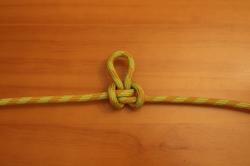
\includegraphics[width=\linewidth]{AugOriginal}
        \caption{Original Image}
        \label{fig:AugOriginal}
	\end{subfigure}
	\begin{subfigure}{.33\textwidth}
		\centering
        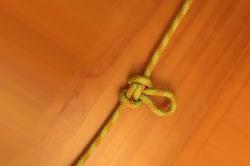
\includegraphics[width=\linewidth]{augmented1}
        \caption{Augmented Image 1}
        \label{fig:Aug1}
	\end{subfigure}
	\begin{subfigure}{.33\textwidth}
		\centering
        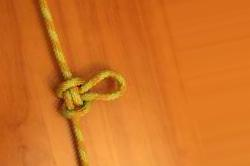
\includegraphics[width=\linewidth]{augmented2}
        \caption{Augmented Image 2}
        \label{fig:Aug2}
	\end{subfigure}
	\begin{subfigure}{.33\textwidth}
		\centering
        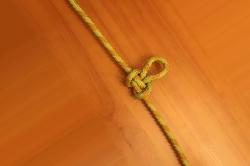
\includegraphics[width=\linewidth]{augmented3}
        \caption{Augmented Image 3}
        \label{fig:Aug3}
	\end{subfigure}
	\begin{subfigure}{.33\textwidth}
		\centering
        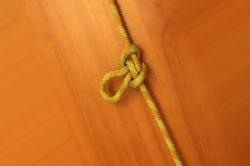
\includegraphics[width=\linewidth]{augmented4}
        \caption{Augmented Image 4}
        \label{fig:Aug4}
	\end{subfigure}
	\begin{subfigure}{.33\textwidth}
		\centering
        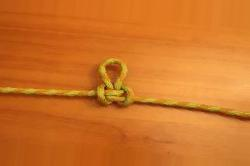
\includegraphics[width=\linewidth]{augmented5}
        \caption{Augmented Image 5}
        \label{fig:Aug5}
	\end{subfigure}
	\caption{Effects of data augmentation on the training dataset}
    \label{fig:DataAugmentationExamples}
\end{figure}

It is then the train and validation generators that are used to fit the model to the training data.

\subsection{Training the Convolutional Neural Network}
To train the convolutional neural network, the model must be fit to the training data.
In Keras, this was achieved by calling the fit\_generator method as shown in Figure \ref{fig:KerasModelTraining}.

\begin{figure}
\caption{Fitting the Model in Keras}
\label{fig:KerasModelTraining}
\begin{lstlisting}

# MODEL FITTING
fit = model.fit_generator(
    train_generator,
    steps_per_epoch=nb_train_samples // batch_size,
    epochs=epochs,
    validation_data=validation_generator,
    validation_steps=nb_validation_samples // batch_size,
    shuffle=True)

# SAVE MODEL (INCLUDING WEIGHTS)
model.save('first_try.h5')


\end{lstlisting}
\end{figure}

The first argument of fit\_generator requires a valid generator that contains the augmented training data.
Therefore, the train\_generator from Figure \ref{fig:KerasDataAugmentationApplication} is the first argument.
The second and third arguments of fit\_generator are steps\_per\_epoch and epochs.
An epoch in Keras is an iteration over a certain number of images from the training dataset.
However, the number of images sampled in every epoch depends on the values of steps\_per\_epoch and batch\_size.
The number of epochs, the value for steps per epoch and the value for batch size can significantly affect the model's training, and they must be selected carefully.
For the implementation, the specified number of epochs was 100, meaning the models would be trained over 100 epochs, and the batch\_size was set to 32.
Therefore, steps\_per\_epoch was set to equal the number of training images divided by the batch\_size of 32 in order to try and obtain an iteration over the entire training dataset for every epoch in training.
This prevented the model from just training on a portion of the training dataset per epoch.
The fourth argument of fit\_generator is validation\_data, which requires the data used to validate the models' performance during training.
Hence, validation\_data was set to equal the validation generator from Figure \ref{fig:KerasDataAugmentationApplication}.
The fifth argument of fit\_generator is validation\_steps.
Similarly to steps\_per\_epoch, validation\_steps specifies the number of batch\_size iterations to perform on the validation data.
Thus, it was set to equal the number of validation images divided by the batch size to try and obtain an iteration over the entire validation dataset per epoch.
This resulted in a more accurate representation of the model's performance during training.
The sixth and final argument of fit\_generator is shuffle, which was set to True.
This is important because it shuffles the training data during training which may discourage patterns to form in the model when its weights are being updated due to the order of the training data.

After the model has been trained via fit\_generator, it can be saved as an HDF5 file with the save method as shown in Figure \ref{fig:KerasModelTraining}.
Once saved, the full trained model and its weights can be later used to predict class labels on individual images. 


\section{The Knot Classifier iOS App}
The iOS application was implemented to satisfy one of this project's critical requirements, which was that there should be a usable interface through which knots can be classified.
The application was implemented as an iOS application because I own an iPhone and could therefore test the application on my device freely. Also, iOS is currently one of the most popular mobile operating systems, meaning the application could potentially become accessible to many iOS users.
The application itself was implemented in the integrated development environment Xcode with the Swift programming language.

\subsection{Keras to CoreML Model Conversion}
Deep learning models can only be integrated with iOS applications through the Core ML framework.
Furthermore, the Core ML framework can only accept valid Core ML models with a .mlmodel extension to perform machine learning in iOS applications. 
Therefore, in order to implement an iOS application that can classify knots, it was important to first convert the trained convolutional neural network that was saved as an HDF5 file from Keras into a Core ML model.
The convertModel.py Python script was implemented to achieve this.
The code that implemented this conversion is shown in Appendix \ref{appendix:KerastoCoreML}.

As shown in Appendix \ref{appendix:KerastoCoreML}, the coremltools package was used to perform the conversion.
Within the convert method, the ten knot classes were supplied to indicate to the converter that the Keras neural network has a softmax activation as its final layer.
Also, it was extremely important to provide the correct image\_scale of 1/255., as without this, the converted Core ML model could behave differently to the original trained model.
After detailing the correct credentials, the converted model was then saved as knotClassifier.mlmodel with the required .mlmodel extension.
This saved Core ML model could then be dragged into the Knot Classifier Xcode project to enable knot classification results from the trained convolutional neural network.

\subsection{The Knot Classifier Xcode Project}
The main functionality of the Knot Classifier iOS application is located within the ViewController.swift file.
The Swift code from the ViewController.swift file can be seen in Appendix \ref{appendix:SwiftViewController}.
ViewController.swift contains two functions, the viewDidLoad function and the captureOutput function.
ViewController.swift also heavily uses the Vision framework.

The viewDidLoad function is very much equivalent to the main function found in languages such as Java or Python in the sense that the app's logic all begins in viewDidLoad.
The first thing viewDidLoad implements is the AVCaptureSession, which essentially allows the camera's images to be captured in real-time for later analysis by the knotClassifier.mlmodel model.
The input to the capture session is also defined to be the device's camera.
Next, an AVCaptureVideoPreviewLayer is initialised to display the images from the capture session on the screen to the user.
Finally, the capture session's output is set to equal AVCaptureVideoDataOutput().
It is this action that allows the captureOutput function to correctly display predictions from the Core ML model based on images from the device's camera.

The captureOutput function is responsible for integrating the knotClassifier.mlmodel into the application.
First of all, a CVPixelBuffer is initialised within captureOutput.
This CVPixelBuffer allows the images from the camera to be analysed pixel by pixel.
Next, the knotClassifier.mlmodel is loaded as VNCoreMLModel.
Thirdly, a VNCoreMLRequest is set up to display the top 3 VNClassificationObservations predicted by the VNCoreMLModel to a predictionOutput label.
The predictionOutput label is the label responsible for the displaying the classification labels and their corresponding prediction accuracy.
The predictionOutput label must be updated on the main thread, therefore it is dispatched to the main queue.
Finally, the request is performed by the VNImageRequestHandler, with the CVPixelBuffer supplying the data.

The resulting application has the interface shown in Figure \ref{fig:IntroApp} and the classification results are displayed in real-time along with their corresponding probability.
Of course, the classification results mirror the input images supplied by the device's camera in real-time. 


%---------------------------------------------

% EVALUATION

\chapter{Evaluation}

The purpose of the evaluation was to determine whether or not the project's critical requirements had been satisfied, and to analyse answers that were given for each question that was first mentioned in the project's scope.
Hence, the evaluation was split into many sections, where each section attempts to answer a specific question laid out in the project's scope and requirements that were defined earlier in the project.
It should also be noted that the experimental figures will appear at the end of this chapter to promote easier reading.

\section{What features affect the classification of knots?}

Neural networks can certainly resemble black boxes in the sense that they are extremely difficult to fully understand and analyse.
The motivation for figuring out what features of knots affect the classification accuracy and what features of the model architecture affect the classification accuracy is to gain precious insight into what the convolutional neural network is doing/analysing when it is learning to classify knot topology.
To answer this question, this section has been split into two parts, where one part explores the dataset features and the other part explores the model architecture features.  

\subsection{Dataset}
The dataset features that will be explored have been reflected and selected by the design and implementation of the datasets.
The datasets have been organised to consider knot tension, knot lighting, knot background and knot z-axis rotation.
Every following subsection will explore one of these features individually in order to paint a complete picture of what individual features are important to the classification performance.
In order to effectively test what individual features affect the classification performance, all trained convolutional neural networks will be validated on a constant validation dataset that consists of controlled and wild knot images.
The only differing variable for each experiment will be the training dataset used to train each convolutional neural network.
Furthermore, for each of the following experiments, the changing training dataset always contains 390 images (39 images per knot class), and the constant validation set always contains the same 120 images (12 images per knot class).
It is also important to mention that these experiments were run for 100 epochs and did not incorporate data augmentation, in an attempt to obtain a clear result of the features of the knots. 

\subsubsection{Knot Tension Experiment}
It was originally hypothesised that if the medium model was trained on three different training datasets, where each dataset differed by knot tension alone, and was validated on a constant validation dataset, where the validation dataset contains a subset of the overall controlled and wild datasets, then each model would have a different training history where each model shows a different level of generalisation or overfitting.

The medium-sized convolutional neural network architecture was trained on three different datasets.
The first dataset contained images of knots tied only at a set tension.
The second dataset contained images of knots tied only at a loose tension.
The third dataset contained images of knots tied only at a very loose tension.
The training history plots of each individual experiment were then compared to determine whether a difference has been caused due to knot tension.
The experimental results appear in Figure \ref{fig:KnotTensionResults}.

\begin{figure}[h]
	\begin{subfigure}{\textwidth}
		\centering
        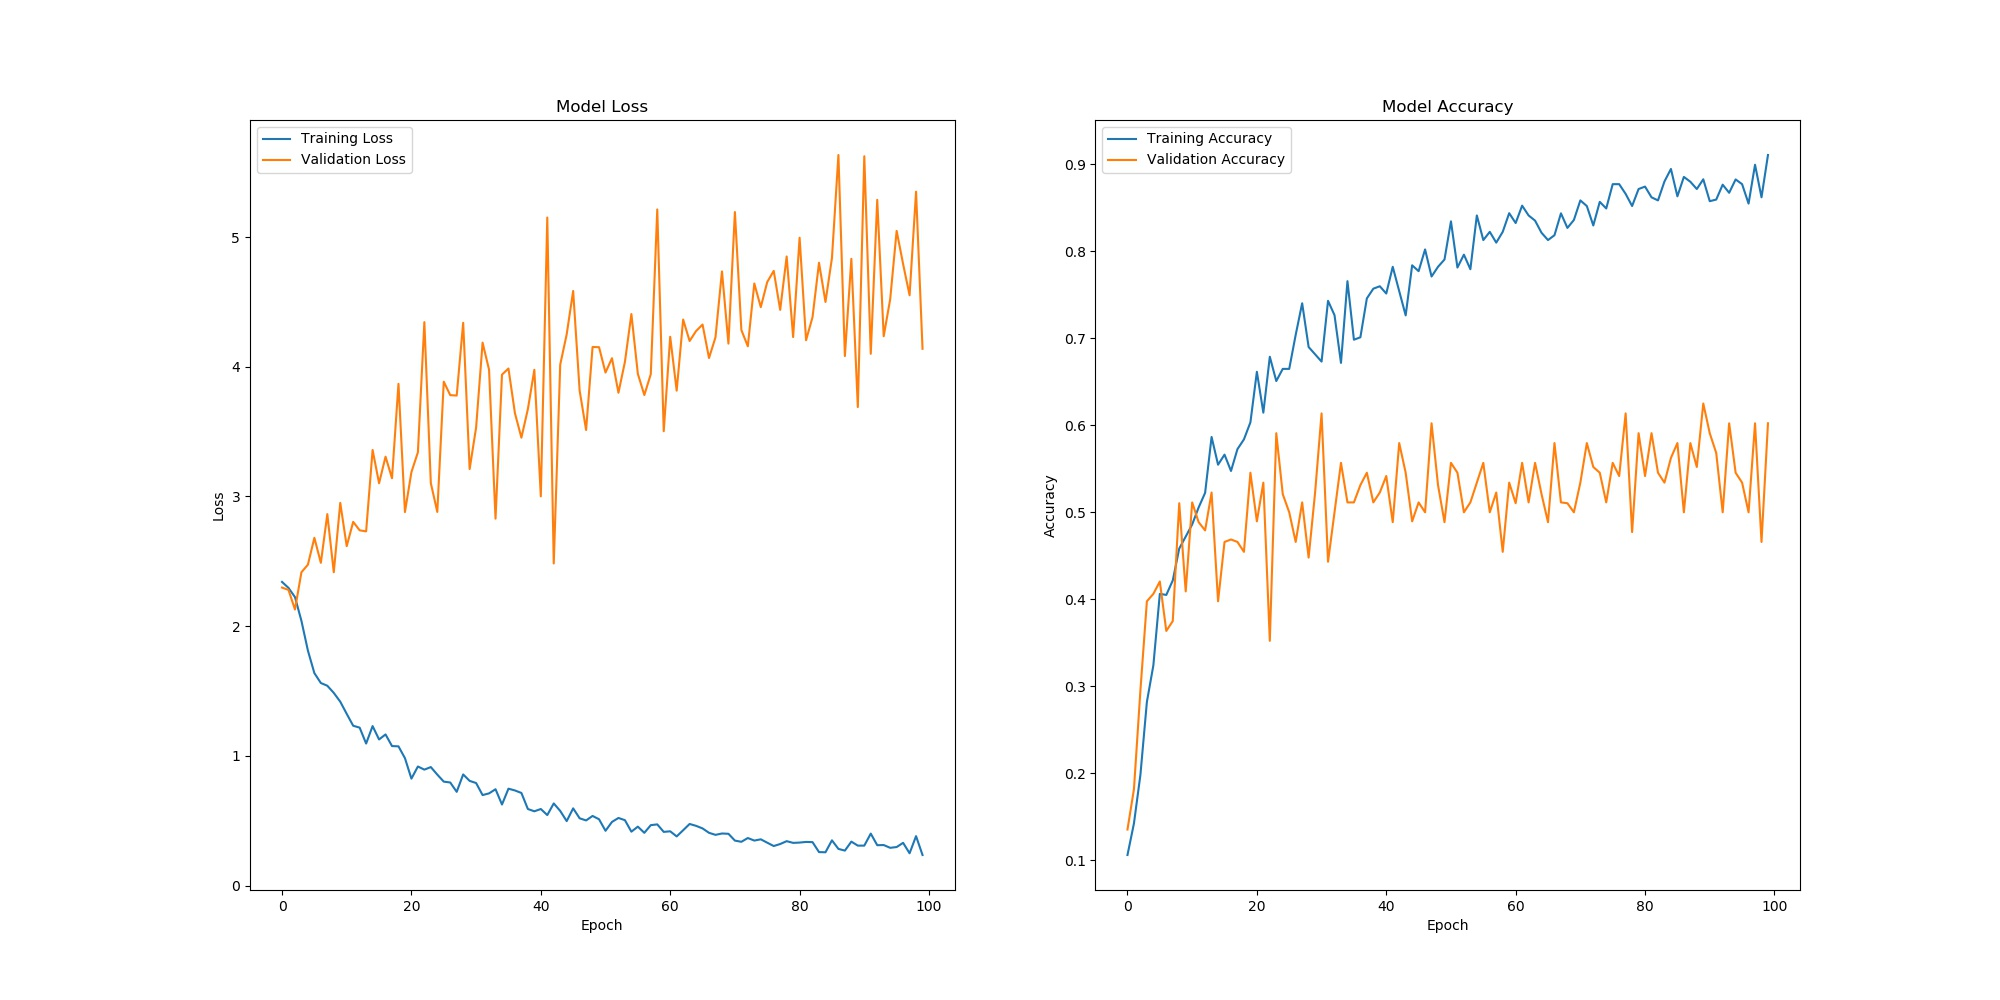
\includegraphics[width=.8\linewidth]{eval/setTensionResult}
        \caption{Set Tension Training History}
        \label{fig:SetTensionExperiment}
	\end{subfigure}
	\begin{subfigure}{\textwidth}
		\centering
        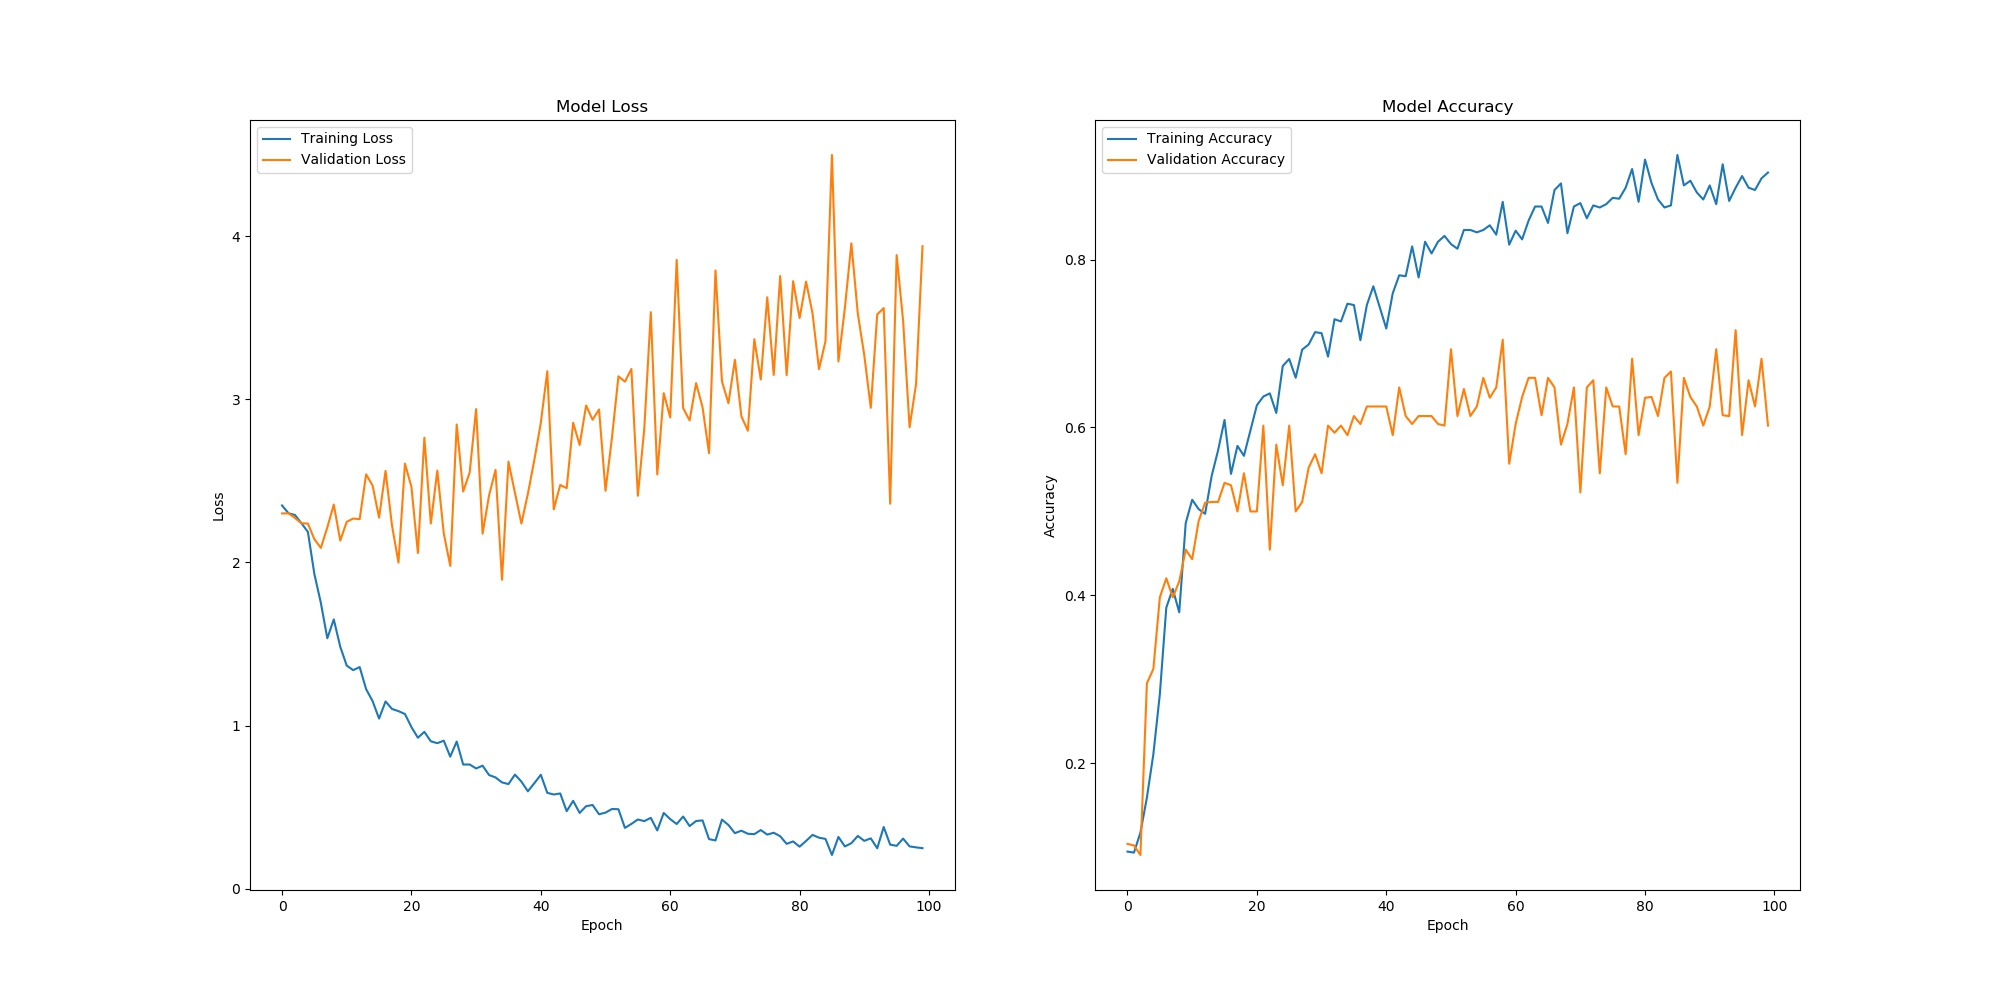
\includegraphics[width=.8\linewidth]{eval/looseTensionResult}
        \caption{Loose Tension Training History}
        \label{fig:LooseTensionExperiment}
	\end{subfigure}
	\begin{subfigure}{\textwidth}
		\centering
        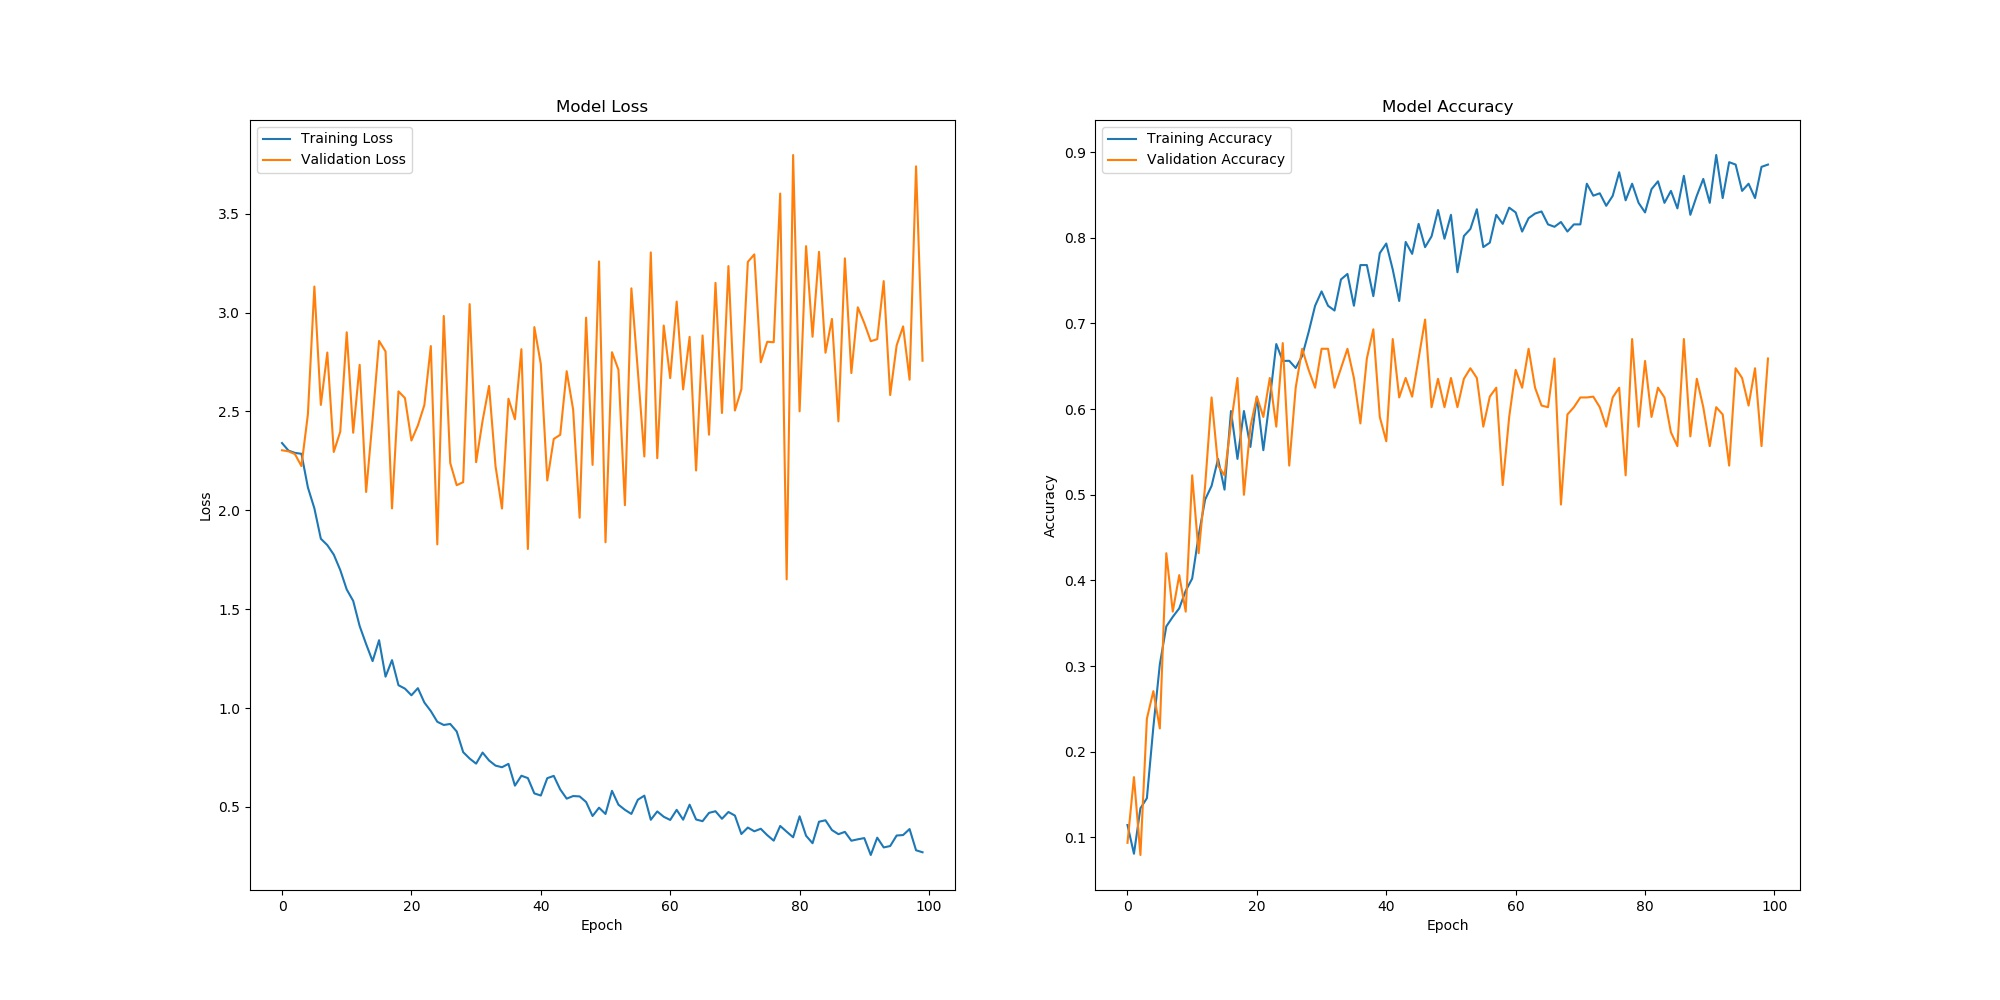
\includegraphics[width=.8\linewidth]{eval/veryLooseTensionResult}
        \caption{Very-Loose Tension Training History}
        \label{fig:VeryLooseExperiment}
	\end{subfigure}
	\caption{Results of the Knot Tension Experiment}
    \label{fig:KnotTensionResults}
\end{figure}

From the training history plots shown in Figure \ref{fig:KnotTensionResults} it is clear to see that the training history for each model was quite similar, even with the different training datasets. However, it is also clear to see that each model began to significantly overfit to the training data, and so the validation loss gradually increased for every epoch of training which also hampered the validation accuracy. Considering that the validation dataset contained images of knots tied at different tensions, the results of this experiment indicate that the medium model struggles to generalise to this training data when trained on a dataset containing knots tied at only one specific tension. This result justifies the decision to capture each knot tied at different tensions within the controlled dataset. 

\subsubsection{Knot Lighting Experiment}
It was originally hypothesised that if the medium model was trained on three different training datasets, where each dataset differed by lighting alone, and was validated on a constant validation dataset, where the validation dataset contains a subset of the overall controlled and wild datasets, then each model would have a different training history where each model shows a different level of generalisation or overfitting.

The medium-sized convolutional neural network architecture was trained on three different datasets.
The first dataset contained images of knots in diffuse lighting conditions.
The second dataset contained images of knots in side-lit lighting conditions.
The third dataset contained images of knots in directly-lit lighting conditions.
The training history plots of each individual experiment will then be compared to determine whether a difference has been caused due to differing lighting conditions.
The experimental results appear in Figure \ref{fig:KnotLightingResults}.

\begin{figure}[h]
	\begin{subfigure}{\textwidth}
		\centering
        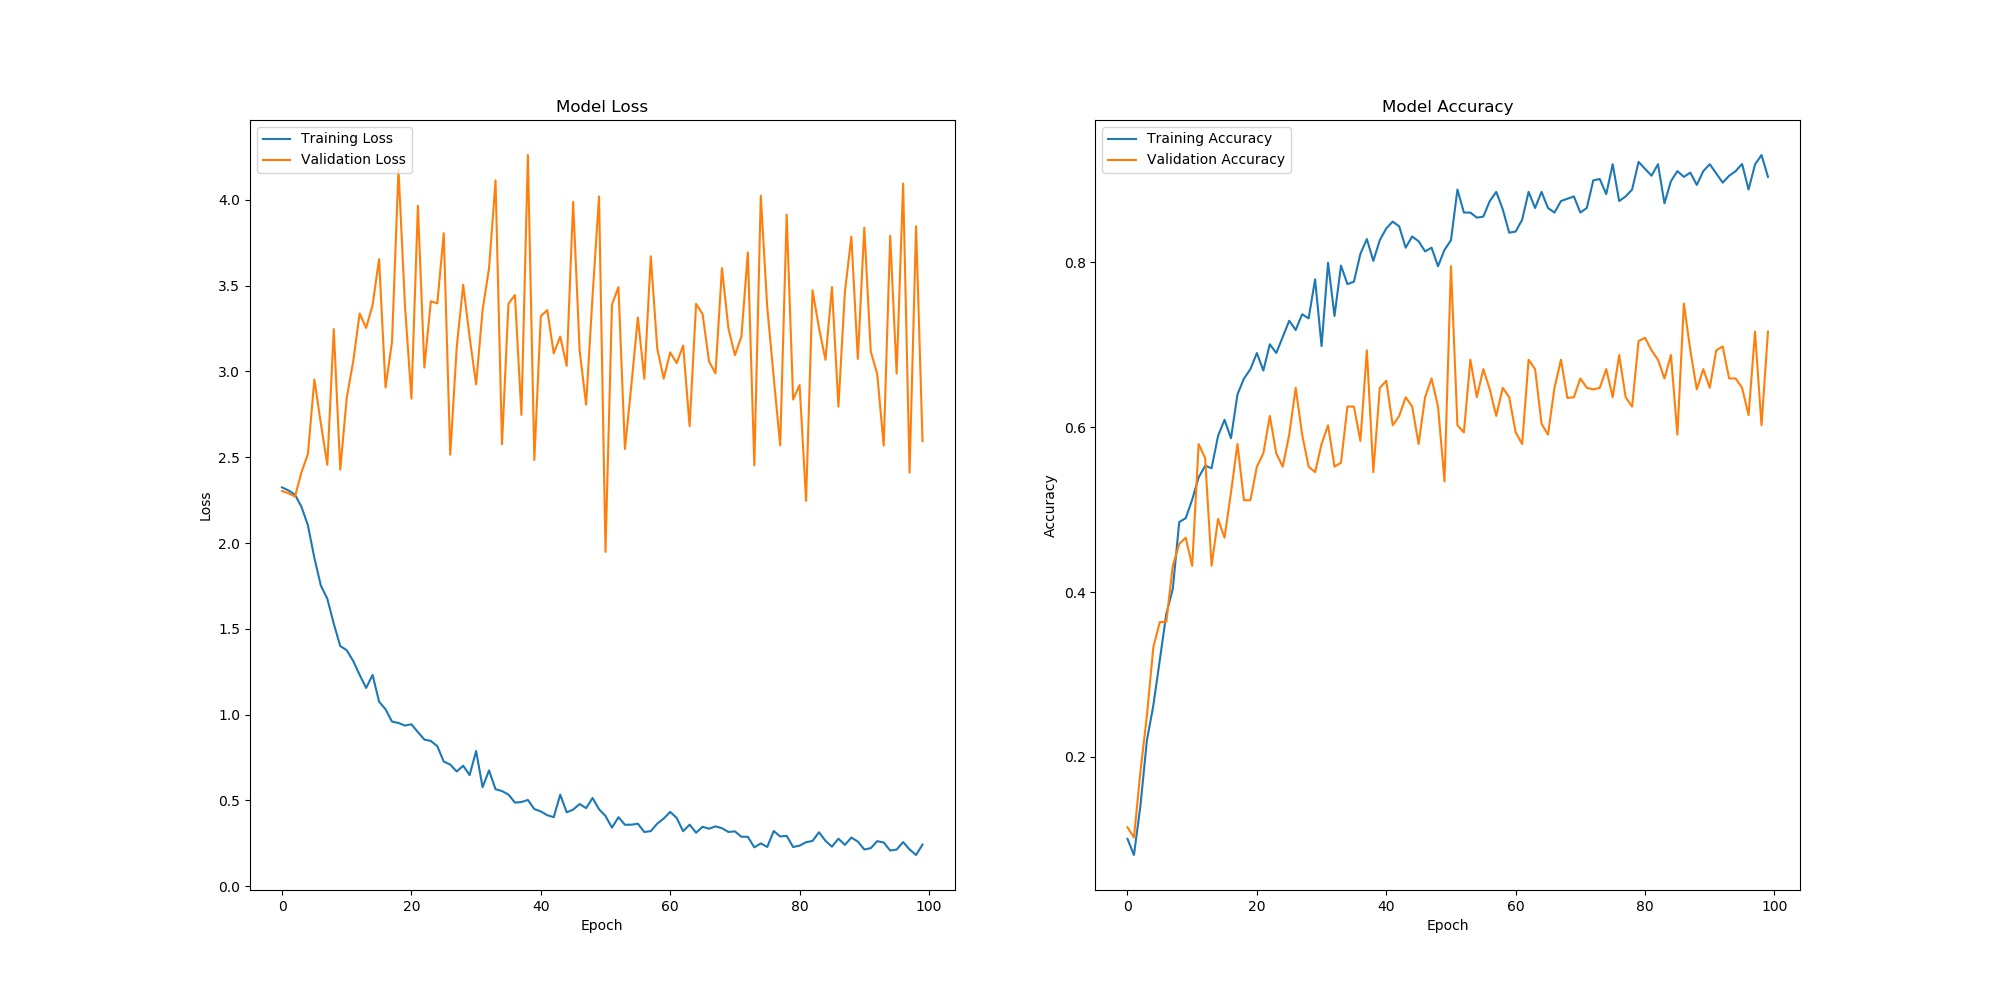
\includegraphics[width=.8\linewidth]{eval/diffuseLightResult}
        \caption{Diffuse Light Training History}
        \label{fig:DiffuseLightingExperiment}
	\end{subfigure}
	\begin{subfigure}{\textwidth}
		\centering
        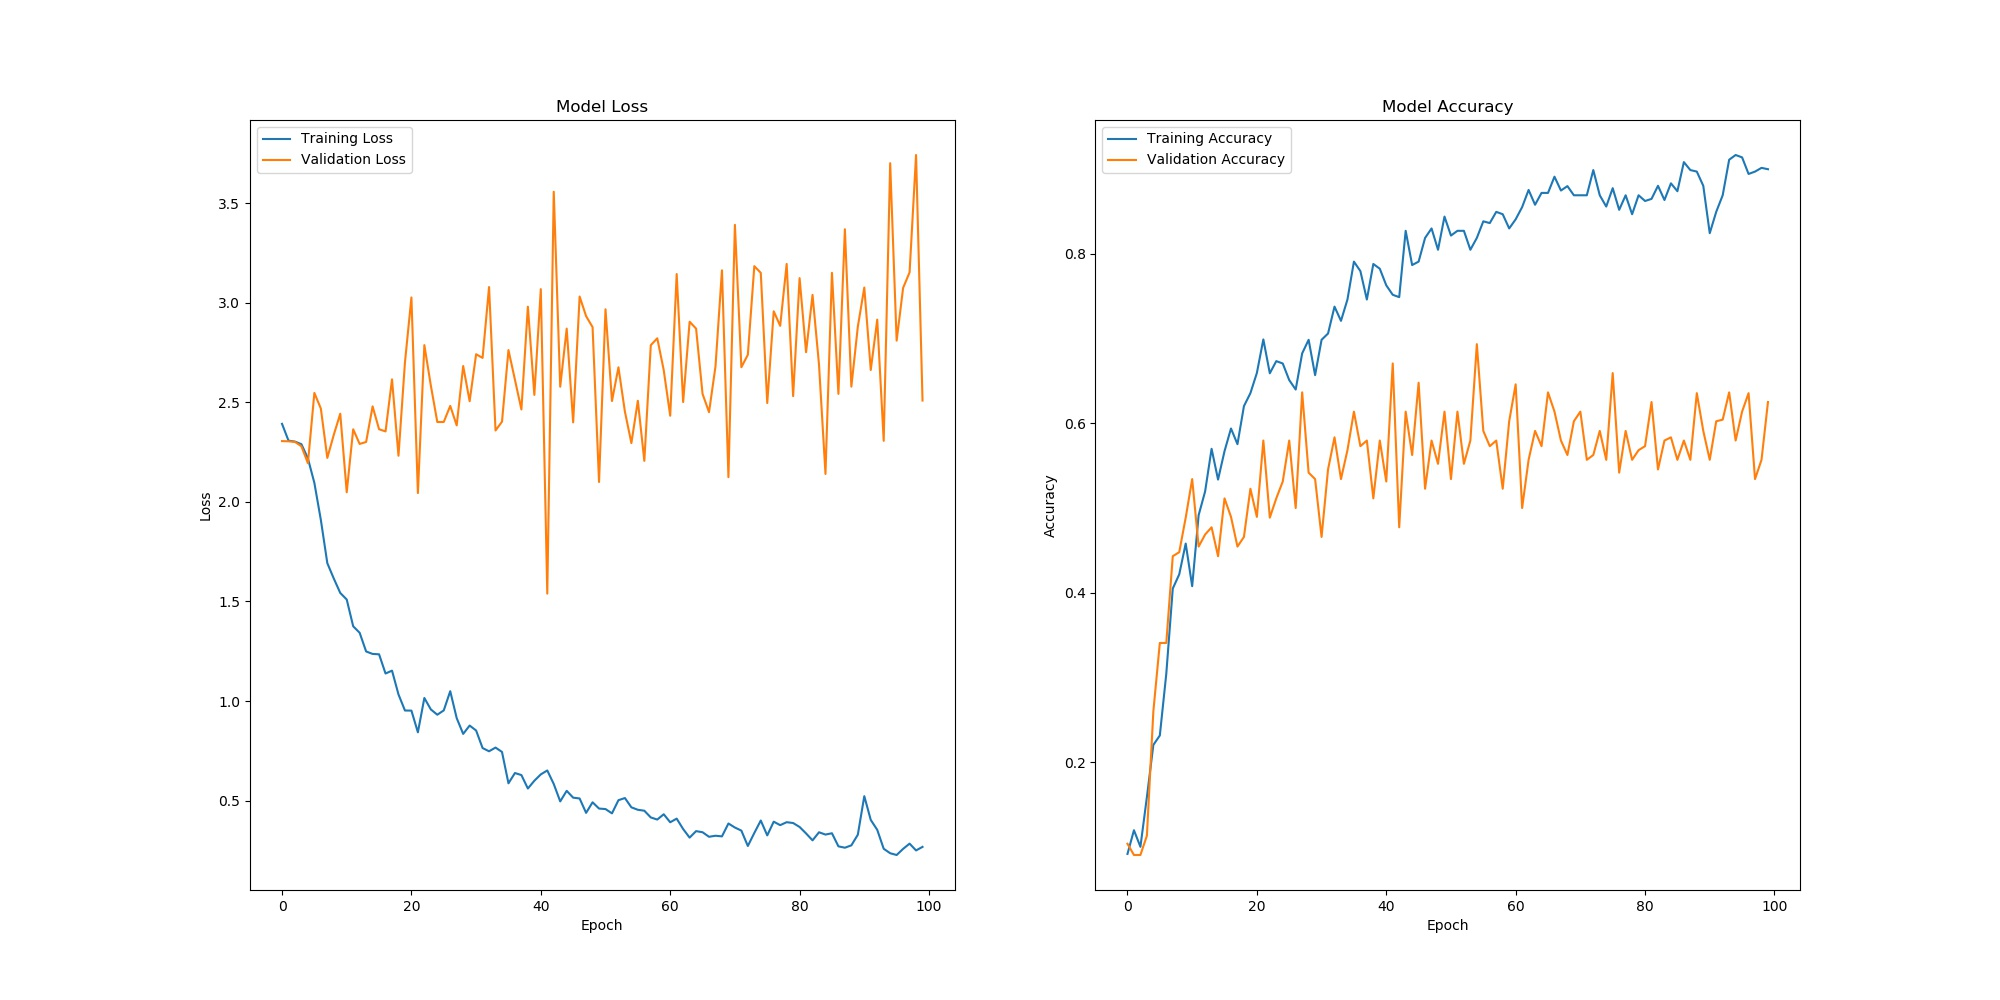
\includegraphics[width=.8\linewidth]{eval/aboveLightResult}
        \caption{Direct Light Training History}
        \label{fig:AboveLightingExperiment}
	\end{subfigure}
	\begin{subfigure}{\textwidth}
		\centering
        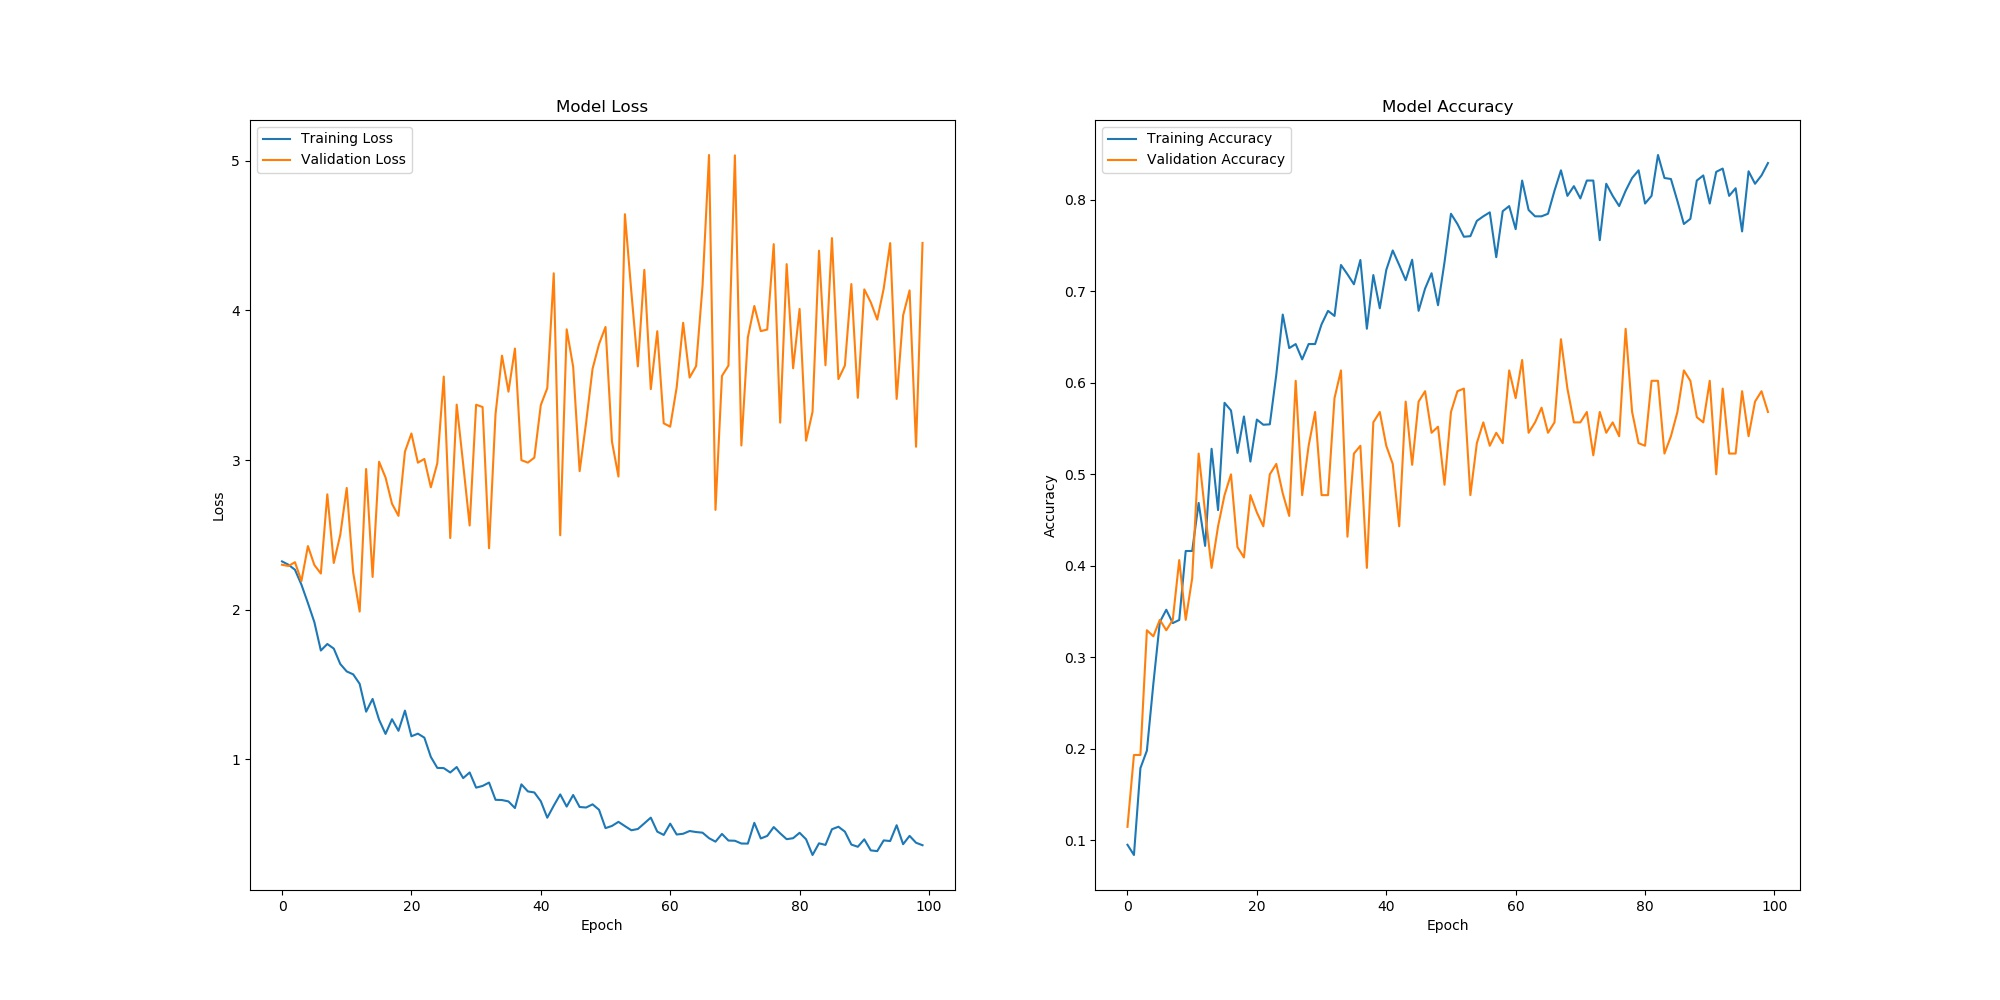
\includegraphics[width=.8\linewidth]{eval/sideLightResult}
        \caption{Side Light Training History}
        \label{fig:SideLightingExperiment}
	\end{subfigure}
	\caption{Results of the Knot Lighting Experiment}
    \label{fig:KnotLightingResults}
\end{figure}

From the training history plots shown in Figure \ref{fig:KnotLightingResults} it is clear to see that the training history for each model was quite similar, even with the different training datasets. However, it is also clear to see that each model began to significantly overfit to the training data, and so the validation loss gradually increased for every epoch of training which also hampered the validation accuracy. Considering that the validation dataset contained images of knots tied in different lighting conditions, the results of this experiment indicate that the medium model struggles to generalise to this training data when trained on a dataset containing knots tied in only one specific lighting condition. This result justifies the decision to capture each knot tied in different lighting conditions within the controlled dataset.

\subsubsection{Knot Rotation Experiment}
It was originally hypothesised that if the medium model was trained on three different training datasets, where each dataset differed by z-axis rotation alone, and was validated on a constant validation dataset, where the validation dataset contains a subset of the overall controlled and wild datasets, then each model would have a different training history where each model shows a different level of generalisation or overfitting.

The medium-sized convolutional neural network architecture was trained on two different datasets.
The first dataset contained images of knots tied only at a 0-degree z-axis rotation and a 180-degree z-axis rotation.
The second dataset contained images of knots tied only at a 90-degree z-axis rotation and a 270-degree z-axis rotation.
The training history plots of each individual experiment will then be compared to determine whether a difference has been caused due to knot z-axis rotation.
The experimental results appear in Figure \ref{fig:KnotRotationResults}.

\begin{figure}[h]
	\begin{subfigure}{\textwidth}
		\centering
        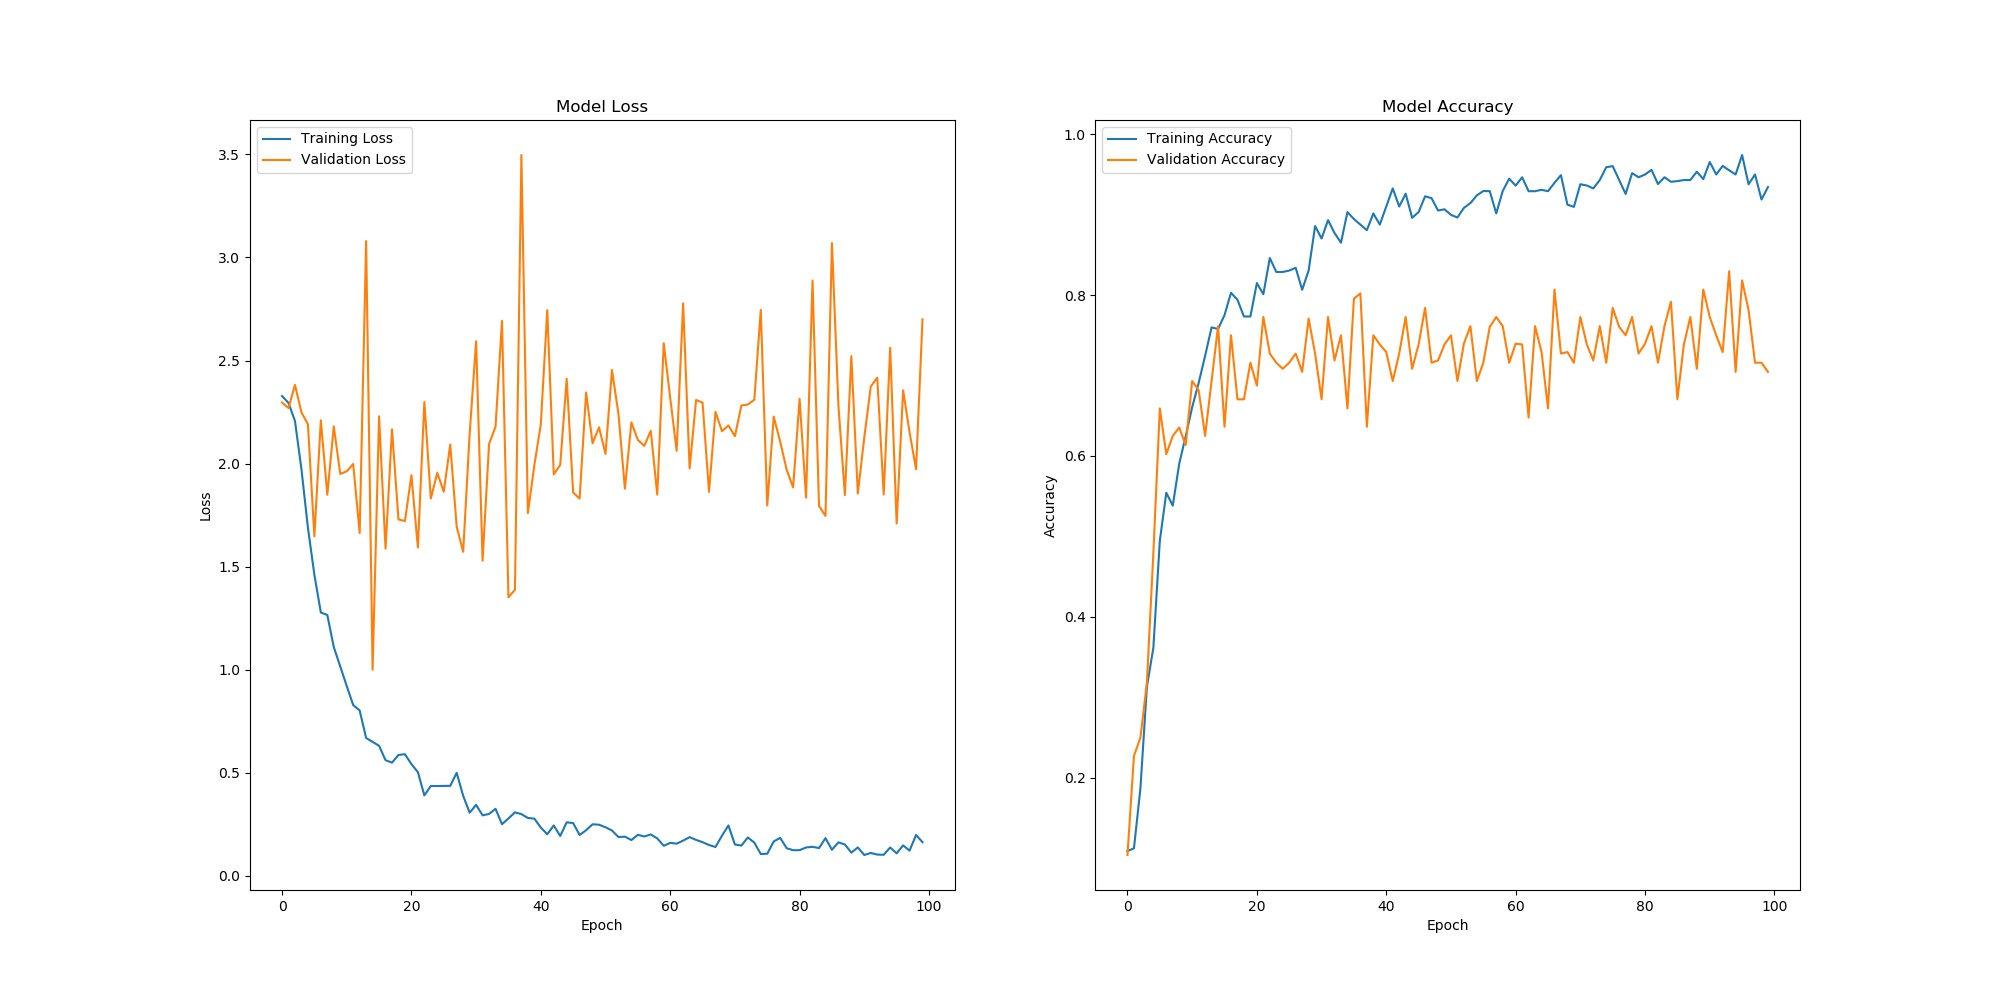
\includegraphics[width=\linewidth]{eval/faceRotationResult}
        \caption{0 and 180 Degree Rotation Training History}
        \label{fig:FaceRotationExperiment}
	\end{subfigure}
	\begin{subfigure}{\textwidth}
		\centering
        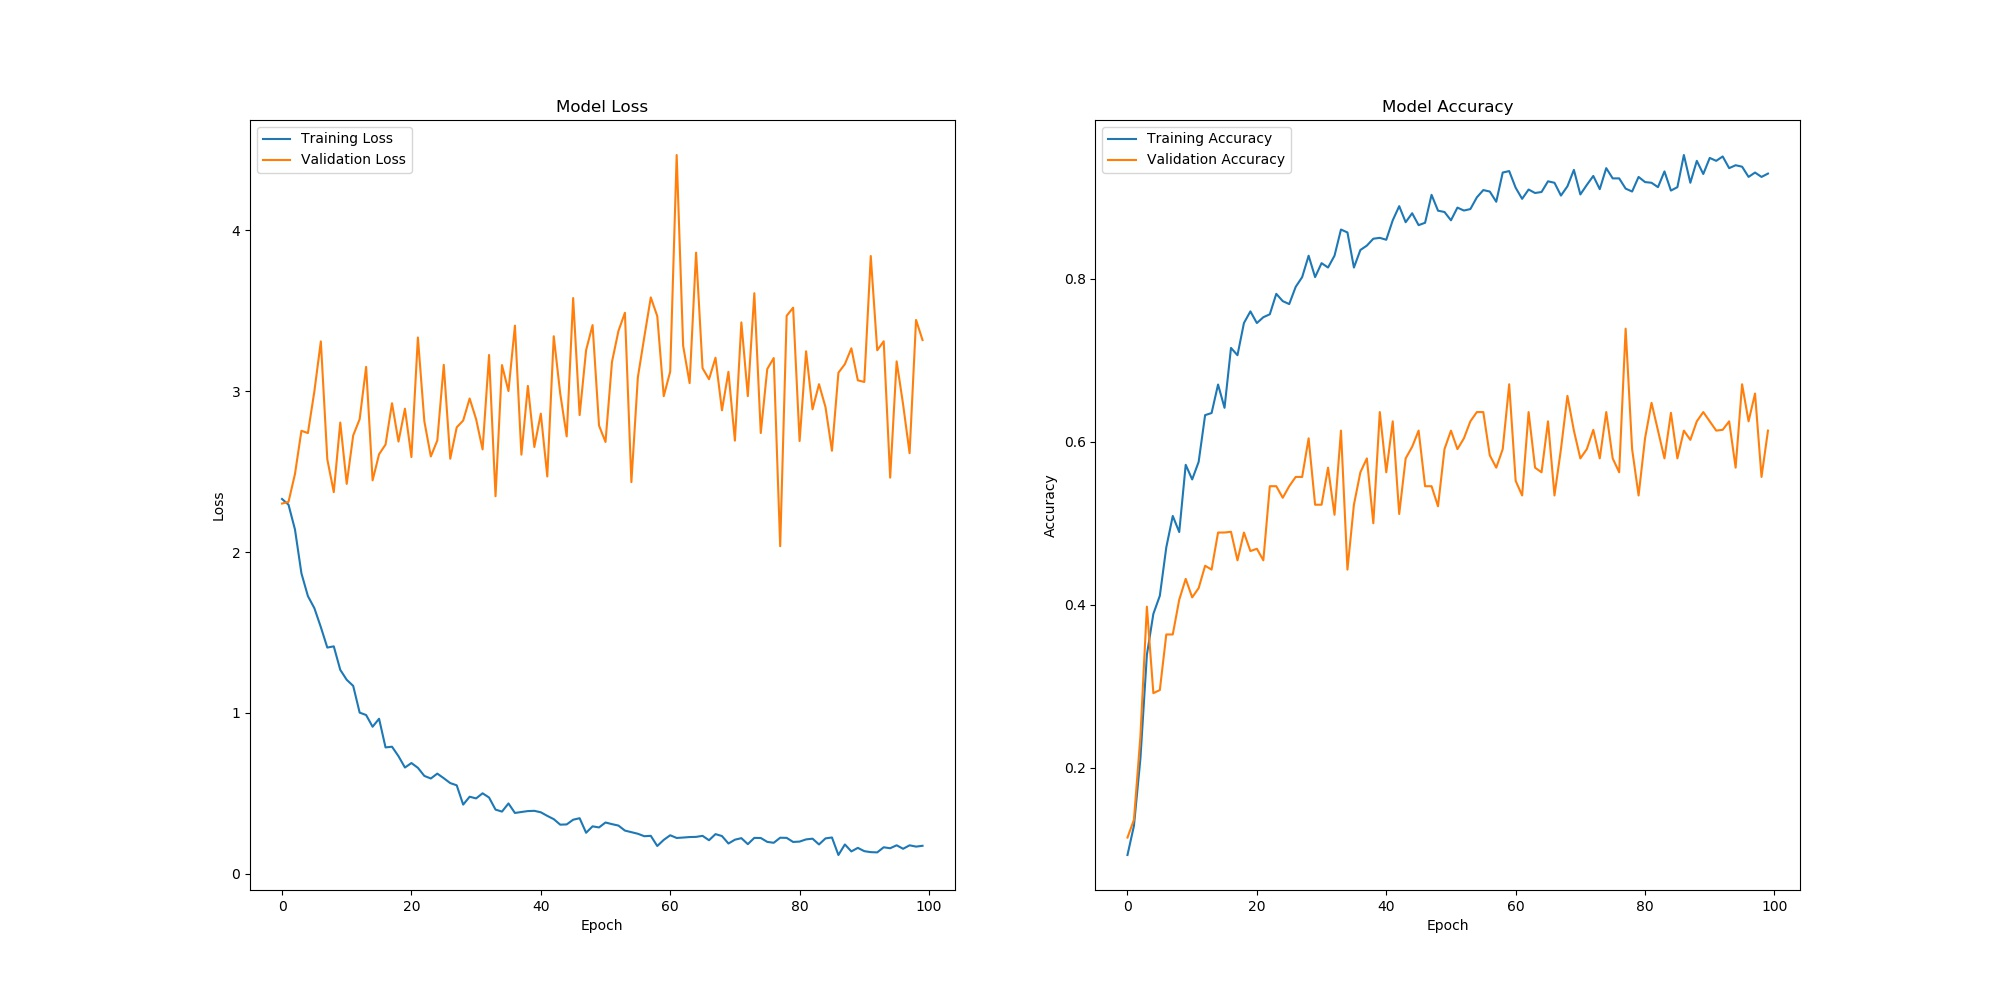
\includegraphics[width=\linewidth]{eval/sideRotationResult}
        \caption{90 and 270 Degree Rotation Training History}
        \label{fig:SideRotationExperiment}
	\end{subfigure}
	\caption{Results of the Knot Rotation Experiment}
    \label{fig:KnotRotationResults}
\end{figure}

From the training history plots shown in Figure \ref{fig:KnotRotationResults} it is clear to see that the training history for each model differed. The validation accuracy was approximately 10\% higher when the model was trained on knots tied at 0 and 180 degrees of z-axis rotation. This result indicates that the rotation of the knot can directly impact on the classification performance of the classifier. It is also clear to see that each model began to significantly overfit to the training data, and so the validation loss gradually increased for every epoch of training which also hampered the validation accuracy. Considering that the validation dataset contained images of knots tied at different rotations, the results of this experiment indicate that the medium model struggles to generalise to this training data when trained on a dataset containing knots tied at only a couple of specific rotations. This result justifies the decision to capture each knot tied at different rotations within the controlled dataset.

\subsubsection{Knot Background Experiment}
It was originally hypothesised that if the medium model was trained on three different training datasets, where each dataset differed by background alone, and was validated on a constant validation dataset, where the validation dataset contains a subset of the overall controlled and wild datasets, then each model would have a different training history where each model shows a different level of generalisation or overfitting.

The medium-sized convolutional neural network architecture was trained on two different datasets.
The first dataset contained images of knots tied with a reflective background.
The second dataset contained images of knots tied with a non-reflective background.
The training history plots of each individual experiment will then be compared to determine whether a difference has been caused due to background.
The experimental results appear in Figure \ref{fig:KnotBackgroundResults}.

\begin{figure}[h]
	\begin{subfigure}{\textwidth}
		\centering
        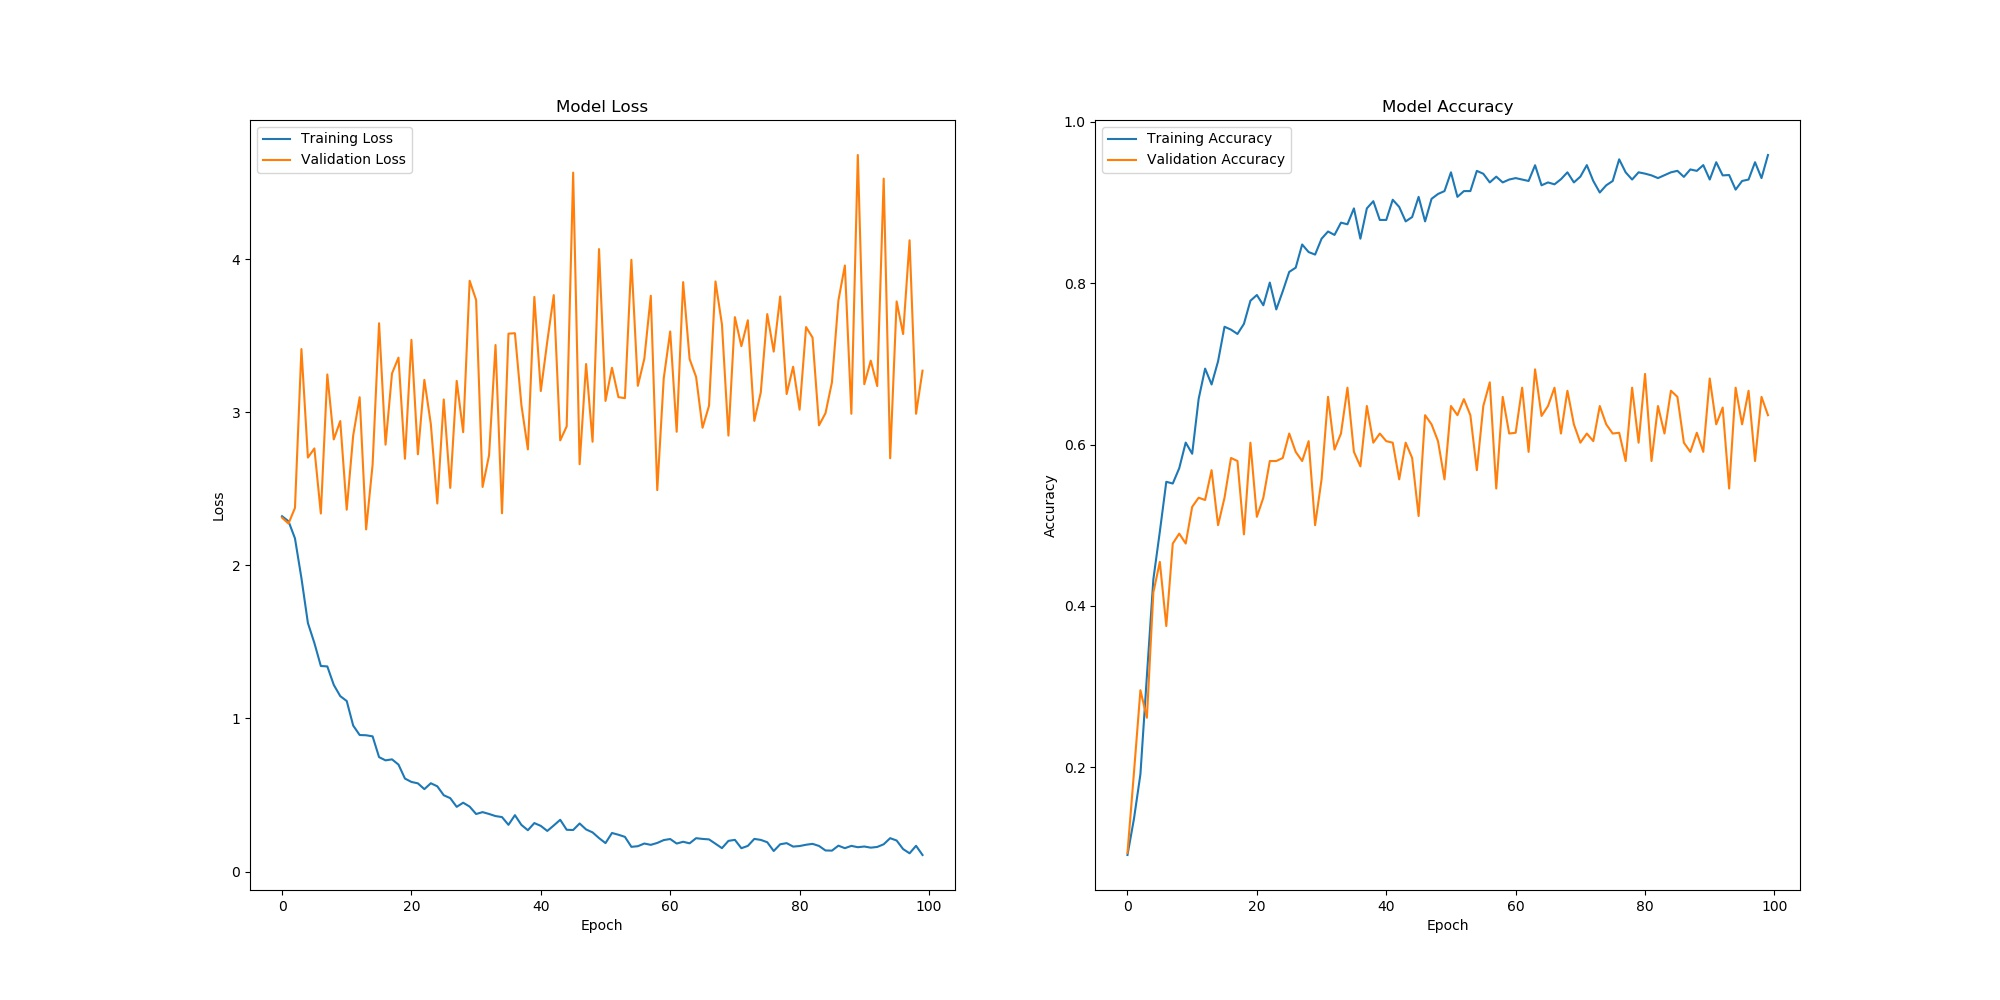
\includegraphics[width=\linewidth]{eval/reflectBackgroundResult}
        \caption{Reflective Background Training History}
        \label{fig:ReflectBackgroundExperiment}
	\end{subfigure}
	\begin{subfigure}{\textwidth}
		\centering
        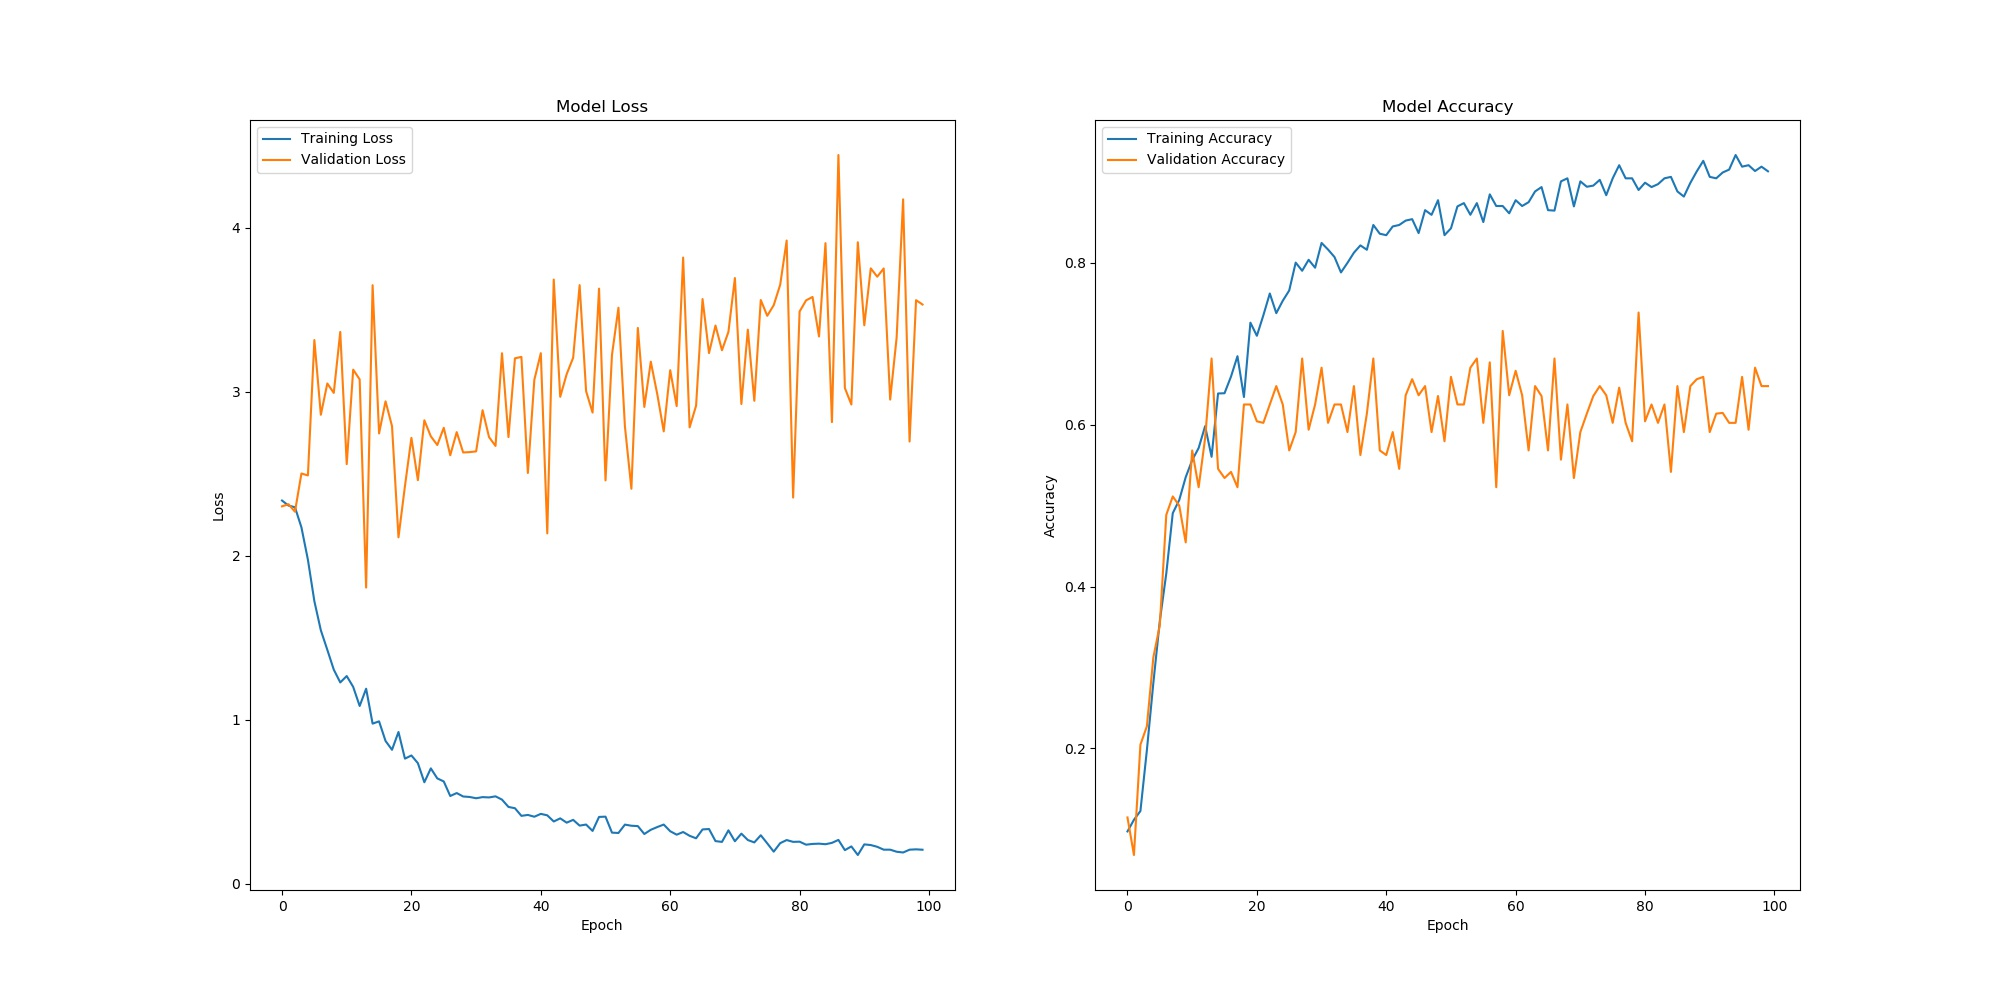
\includegraphics[width=\linewidth]{eval/nonReflectBackgroundResult}
        \caption{Non-Reflective Background Training History}
        \label{fig:NonReflectBackgroundExperiment}
	\end{subfigure}
	\caption{Results of the Knot Background Experiment}
    \label{fig:KnotBackgroundResults}
\end{figure}

From the training history plots shown in Figure \ref{fig:KnotBackgroundResults} it is clear to see that the training history for each model was quite similar, even with the different training datasets. However, it is also clear to see that each model began to significantly overfit to the training data, and so the validation loss gradually increased for every epoch of training which also hampered the validation accuracy. Considering that the validation dataset contained images of knots tied with different backgrounds, the results of this experiment indicate that the medium model struggles to generalise to this training data when trained on a dataset containing knots that were tied with only one specific background. This result justifies the decision to capture each knot tied with different backgrounds within the controlled dataset.

Overall, from these four experiments, it is clear that the rotation of a knot, in particular, can affect the classification performance whereas the knot tension, lighting and background may not affect a classifier as much. However, every experiment has demonstrated that when a model is trained on a dataset of non-changing features, it can struggle to generalise to realistic validation dataset that may contain many variables, thus it is advantageous to train a classifier on a dataset that takes many variables into account.  

\subsection{Model Architecture}
Three different model architectures were designed and implemented based on their number of training parameters.
The small model architecture has 209,482 trainable parameters.
The default medium model architecture has 1,213,098 trainable parameters.
The large model architecture has 9,544,554 trainable parameters.
The aim of this experiment is to analyse how the number of trainable parameters within a model may affect the training and classification performance.
In order to effectively test what individual features affect the classification performance, all trained convolutional neural networks were trained and validated on constant training and validation datasets that consisted of controlled and wild knot images.
The training dataset contained exactly 133 images per knot class, giving a total of 1330 images.
The validation dataset contained exactly 31 images per knot class, giving a total of 310 images.
Each experiment trained the models for 100 epochs with data augmentation enabled.
The only differing variable for each experiment was the convolutional neural network used for training and classifying.
The experimental results appear in Figure \ref{fig:ModelSizeResults}.

\begin{figure}[h]
	\begin{subfigure}{\textwidth}
		\centering
        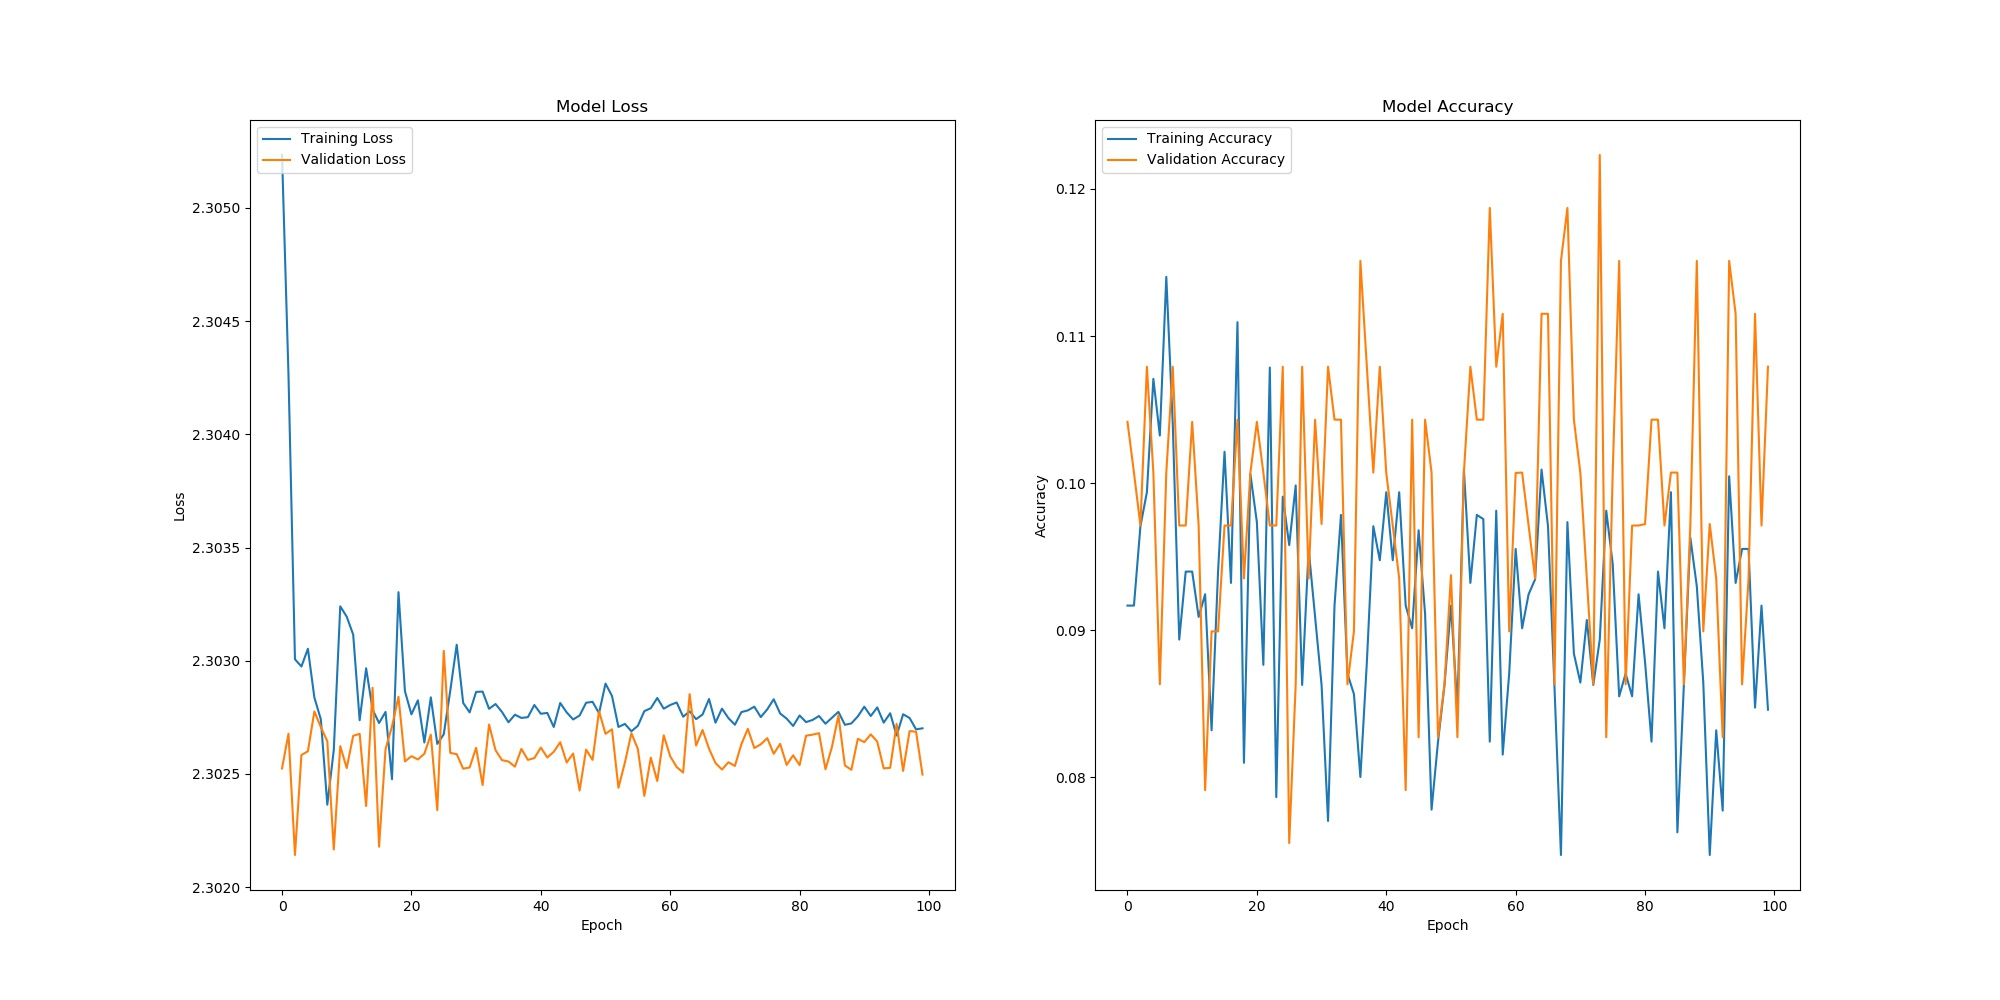
\includegraphics[width=.8\linewidth]{eval/smallModelTrainingHistory}
        \caption{Small Model Training History}
        \label{fig:SmallModelExperiment}
	\end{subfigure}
	\begin{subfigure}{\textwidth}
		\centering
        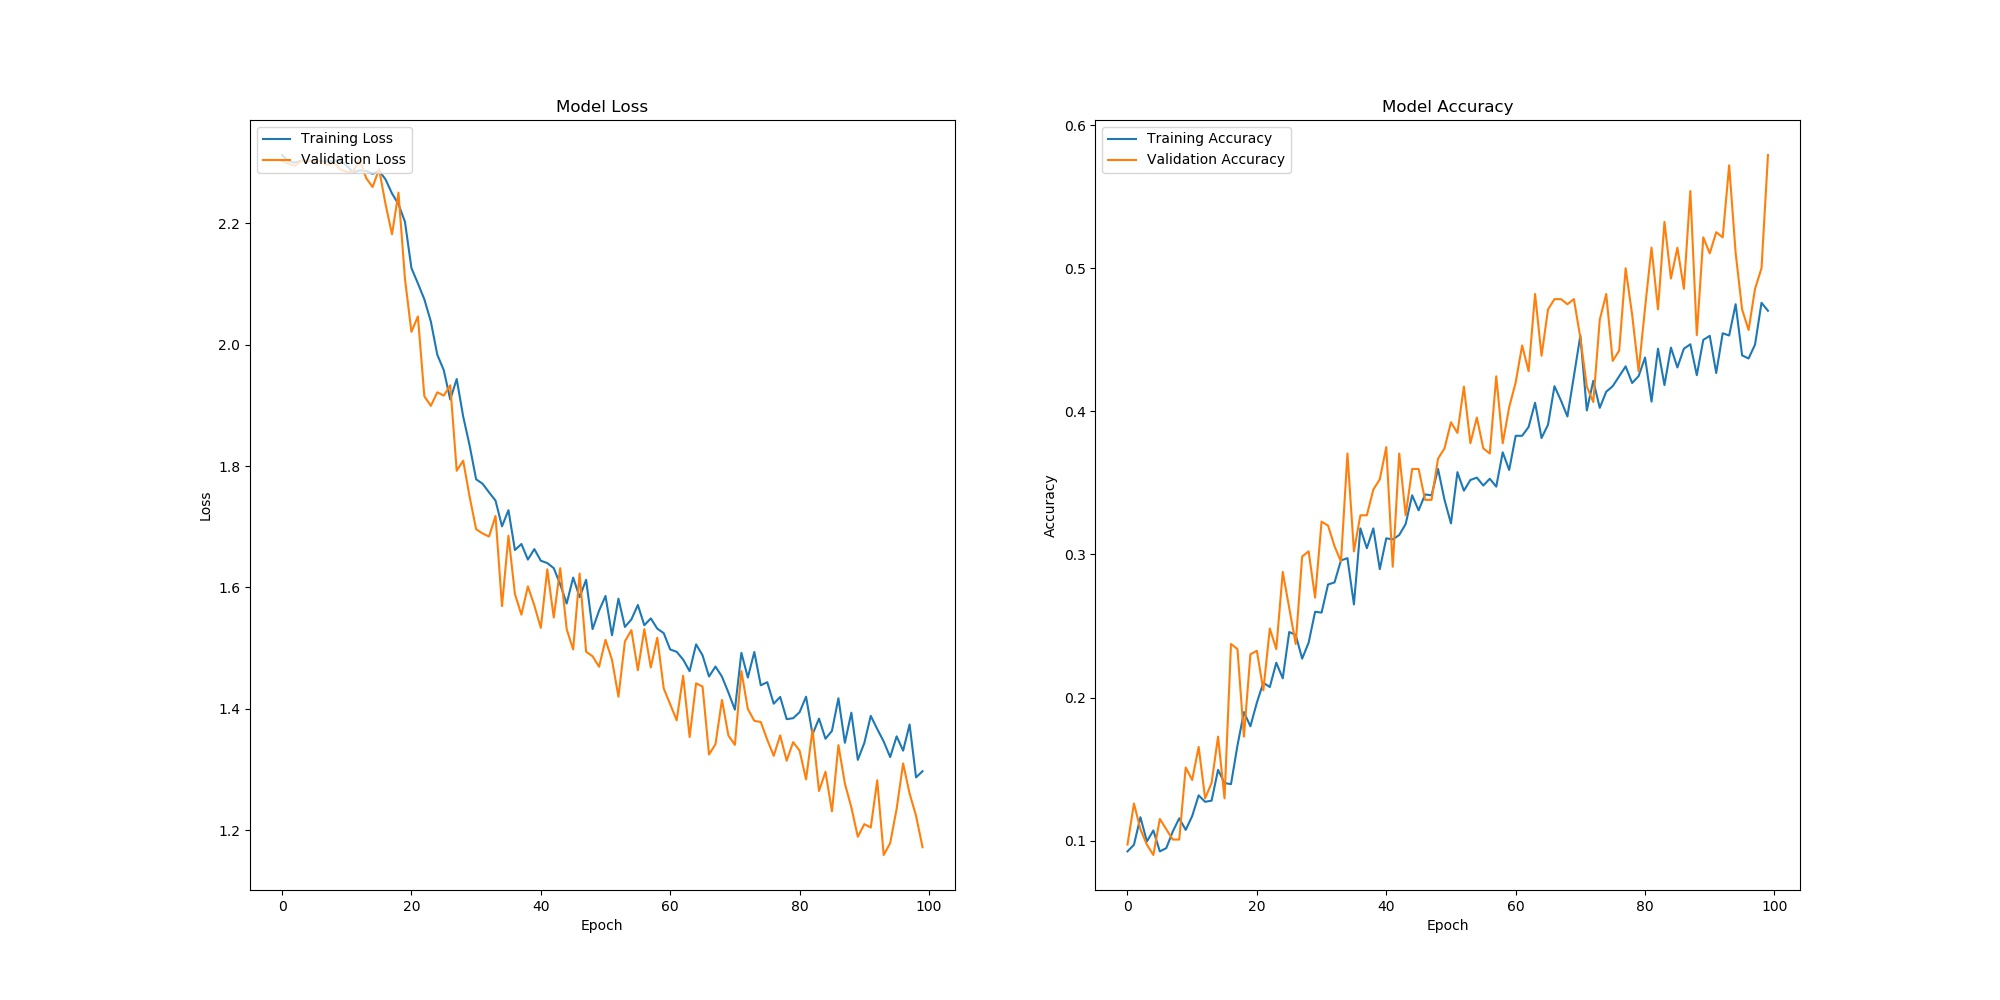
\includegraphics[width=.8\linewidth]{eval/mediumModelTrainingHistory}
        \caption{Medium Model Training History}
        \label{fig:MediumModelExperiment}
	\end{subfigure}
	\begin{subfigure}{\textwidth}
		\centering
        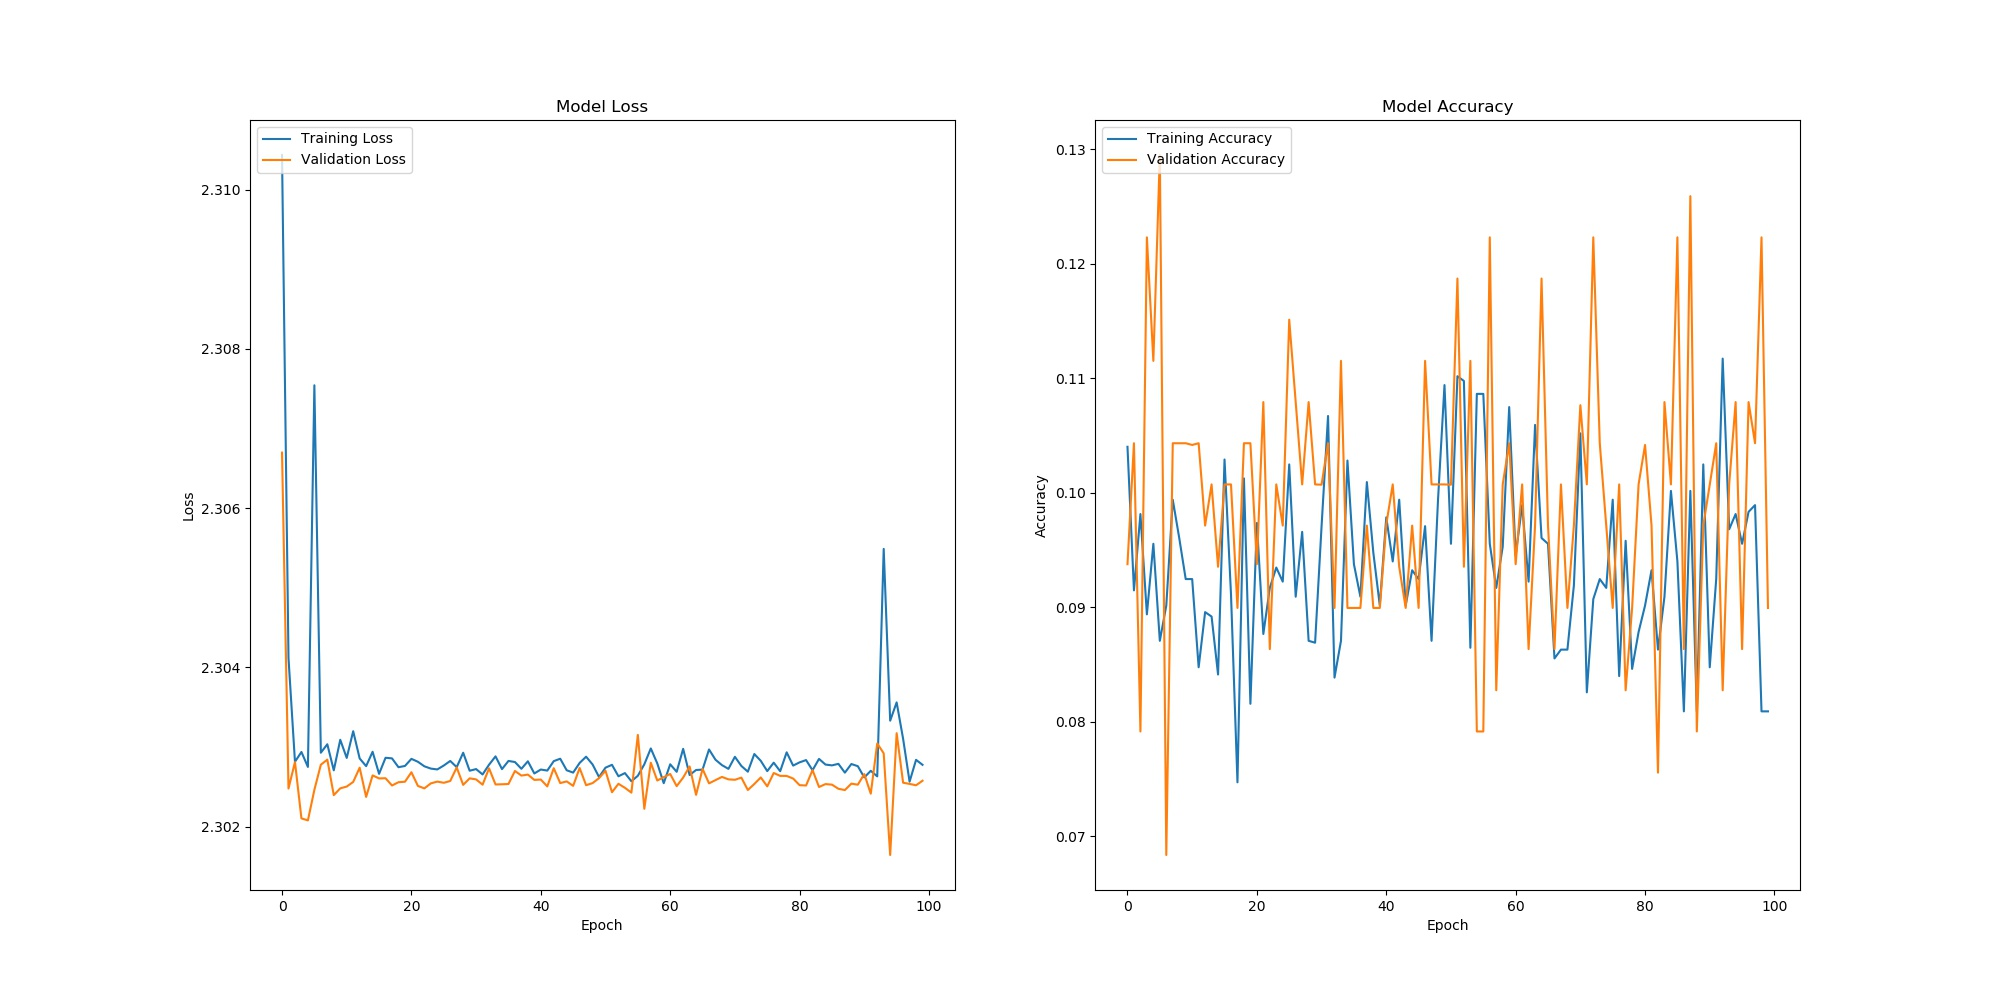
\includegraphics[width=.8\linewidth]{eval/largeModelTrainingHistory}
        \caption{Large Model Training History}
        \label{fig:LargeModelExperiment}
	\end{subfigure}
	\caption{Results of the Model Architecture Experiment}
    \label{fig:ModelSizeResults}
\end{figure}

From the training history plots and the t-SNE visualisation plots in Figure \ref{fig:ModelSizeResults} it is clear to see that the default medium-sized model architecture has the best classification performance when compared to the small and large models. The medium model's validation accuracy is consistently higher than its training accuracy and the medium model's validation loss is consistently lower than its training loss. This shows that the medium model is not overfitting, and is in fact generalising to the validation data. However, the small and large models both struggle to show any sign of productive learning as evident in their training history plots. The training and validation accuracy of these models hovers approximately around 10\%, which is the same accuracy achieved by guessing within a 10-class classification problem.

This experiment has demonstrated that the model architecture and specifically its number of training parameters can significantly impact the classification performance. It is extremely important to build a model that has the right number of training parameters for a specified problem. If there are too little or too many training parameters for the given classification task and its data, then the overall classification performance may suffer.

\section{What techniques successfully combat overfitting?}
When conducting image classification with a small dataset, overfitting is a persistent problem that must be overcome to build a robust classifier.
The 10Knots dataset that was created for this project contains a total of 1440 images for 10 classes, which is certainly small when compared to datasets such as ImageNet\cite{imagenet_cvpr09} and MNIST\cite{lecun-mnisthandwrittendigit-2010} which are used as industry standard computer vision datasets.
As a result, an important aspect of this project was to explore exactly how robust a classifier of this nature can become with such a small dataset.
Hence, it was critical to experiment with two different techniques, namely data augmentation and dropout, that are designed to alleviate overfitting.
This section is split into two sections, where one section explores the effects of data augmentation on the overall classification performance and the other section explores the effects of dropout on the overall classification performance.

\subsection{The Data Augmentation Experiment}
To best determine the effect data augmentation would have on classification, two experiments were undertaken.
The first experiment trained the medium convolutional neural network with no data augmentation for 100 epochs.
The second experiment trained the medium convolutional neural network with data augmentation for 100 epochs.
The training dataset that would be used for both experiments was created by removing approximately 80\% of images from a combination of the controlled 10Knots dataset and the wild dataset.
The validation dataset was then created with the remaining images which equalled approximately 20\% of the original total.
The training dataset contained exactly 133 images per knot class, giving a total of 1330 images.
The validation dataset contained exactly 31 images per knot class, giving a total of 310 images.
The training history plots from each experiment were then compared to provide analysis.
The result from each experiment is shown in Figure \ref{fig:DataAugmentationExperimentResults}.

\begin{figure}[h]
	\begin{subfigure}{\textwidth}
		\centering
        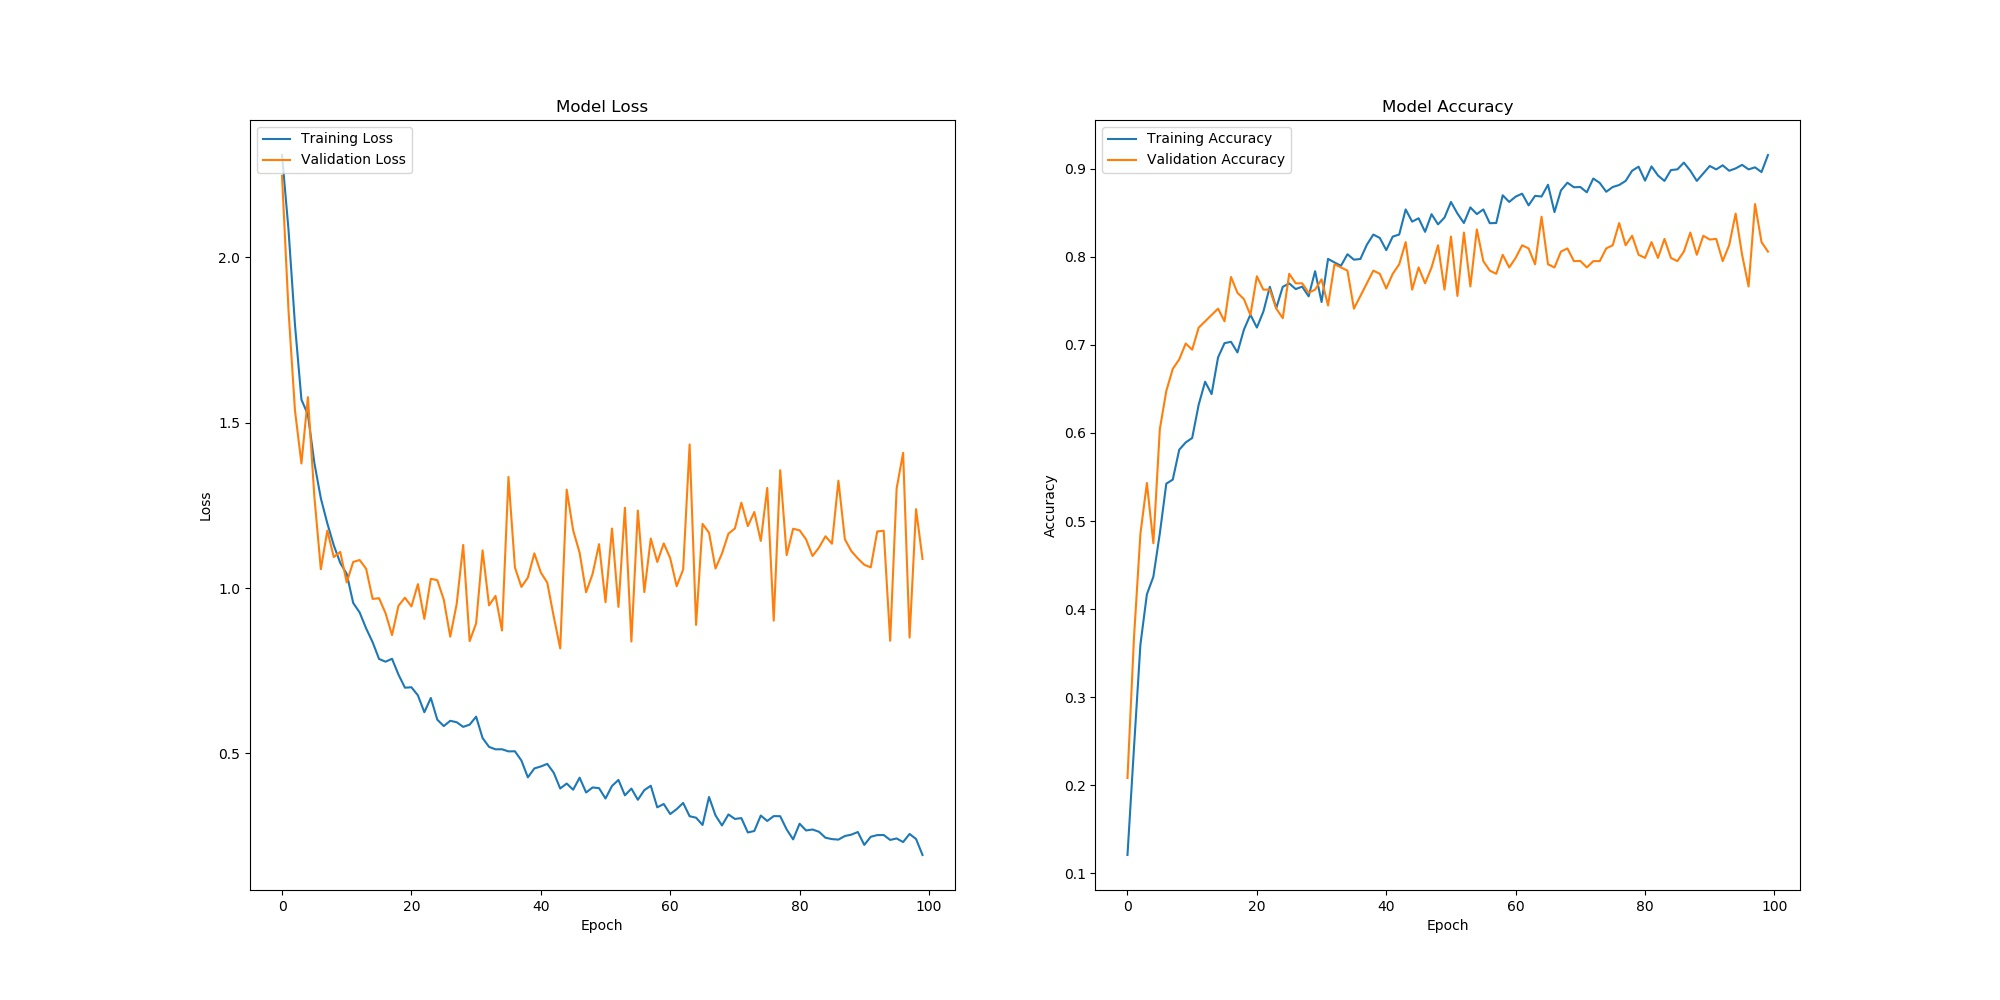
\includegraphics[width=\linewidth]{eval/noAugtrainingHistory}
        \caption{No Data Augmentation Training History}
        \label{fig:NoAugExperiment}
	\end{subfigure}
	\begin{subfigure}{\textwidth}
		\centering
        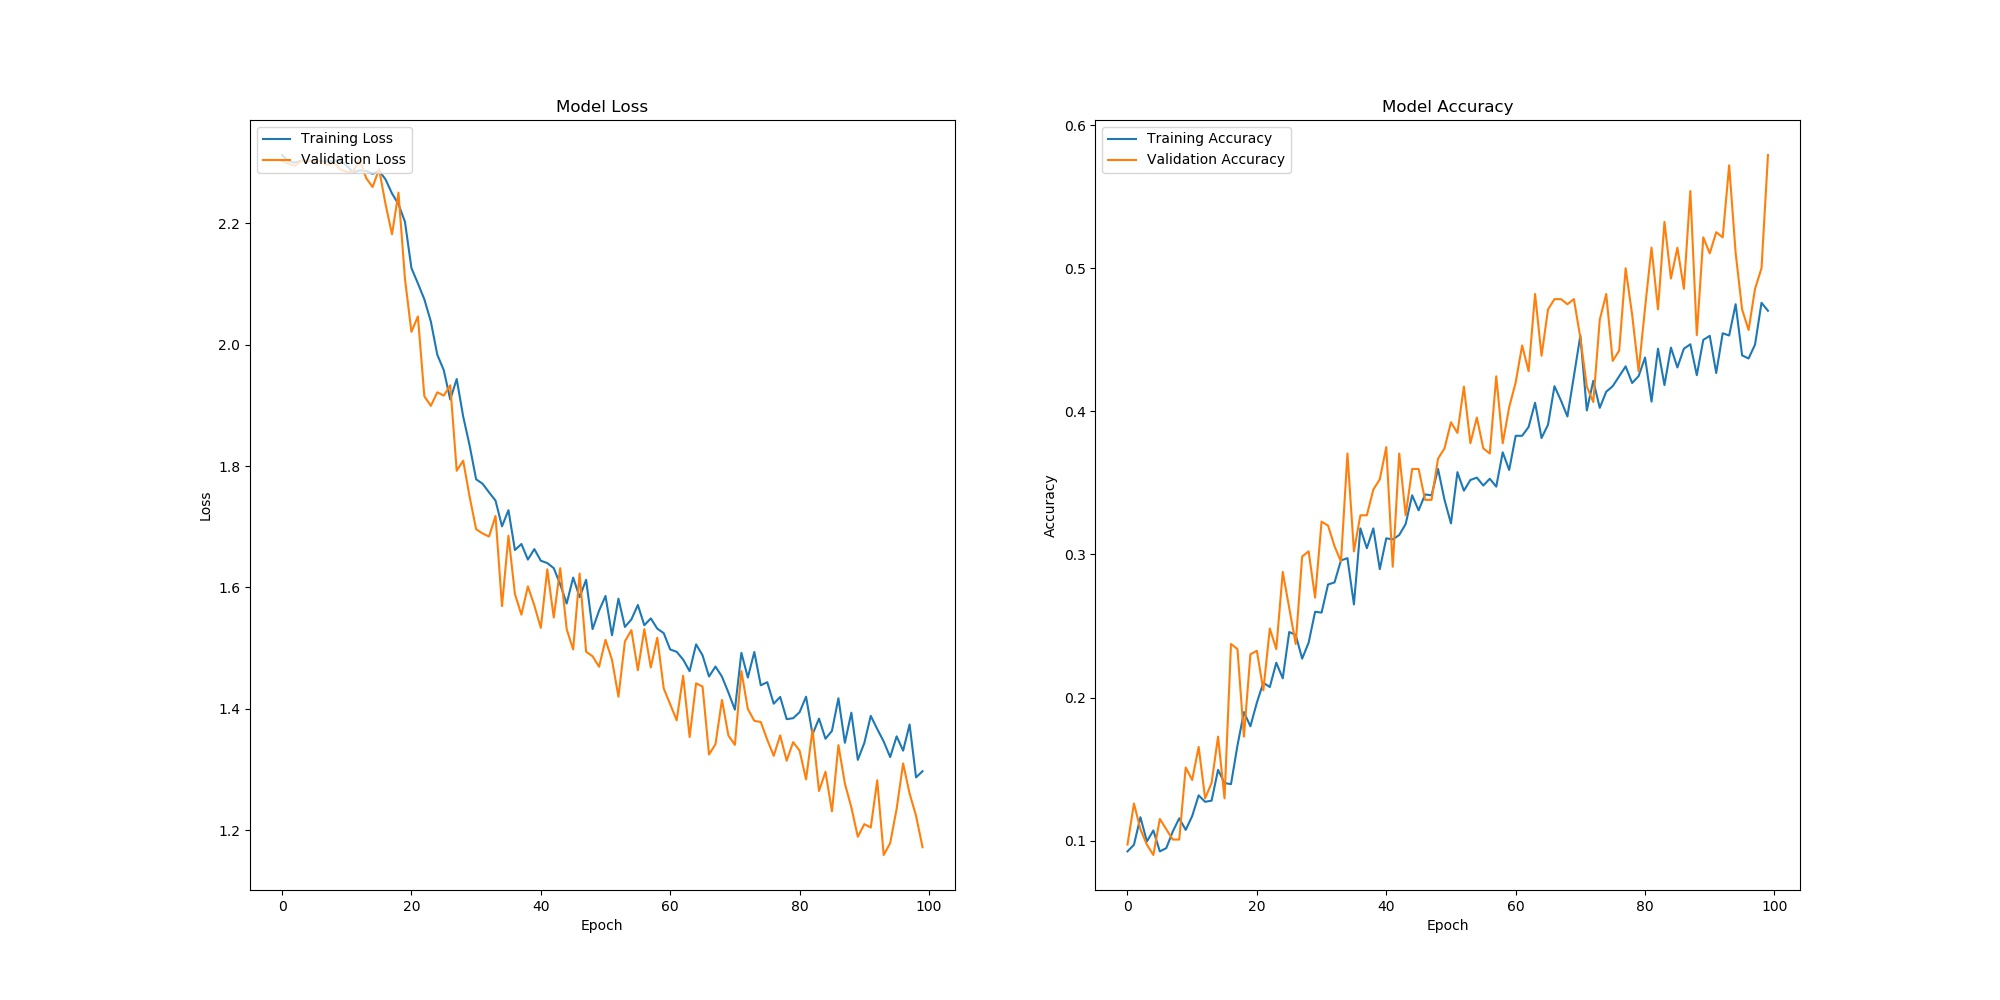
\includegraphics[width=\linewidth]{eval/AugtrainingHistory}
        \caption{Data Augmentation Training History}
        \label{fig:AugExperiment}
	\end{subfigure}
	\caption{Results of the Data Augmentation Experiment}
    \label{fig:DataAugmentationExperimentResults}
\end{figure}

From the training plots within Figure \ref{fig:DataAugmentationExperimentResults}, it is clear that data augmentation has significantly combatted overfitting with respect to this knot classification task. When no data augmentation is applied, the model's validation loss stops decreasing with the training loss at around 20 epochs. This is a classic sign of overfitting. However, with data augmentation applied, the model's validation loss actually decreases more than the training loss for the whole 100 epochs of training, meaning the model has a higher level of generalisation. 

\subsection{The Dropout Experiment}
To best determine the effect dropout would have on classification, two experiments were undertaken.
The first experiment would train the medium convolutional neural network with no dropout and data augmentation for 100 epochs.
The dropout was removed from the network by simply commenting out the lines of code that initialised the dropout layers.
The second experiment would train the medium convolutional neural network with dropout and data augmentation for 100 epochs.
The training dataset that would be used for both experiments was created by removing approximately 80\% of images from a combination of the controlled 10Knots dataset and the wild dataset.
The validation dataset was then created with the remaining images which equalled approximately 20\% of the original total.
The training dataset contained exactly 133 images per knot class, giving a total of 1330 images.
The validation dataset contained exactly 31 images per knot class, giving a total of 310 images.
The training history plots from each experiment were then compared to provide analysis.
The result from each experiment is shown in Figure \ref{fig:DropoutExperimentResults}.

\begin{figure}[h]
	\begin{subfigure}{\textwidth}
		\centering
        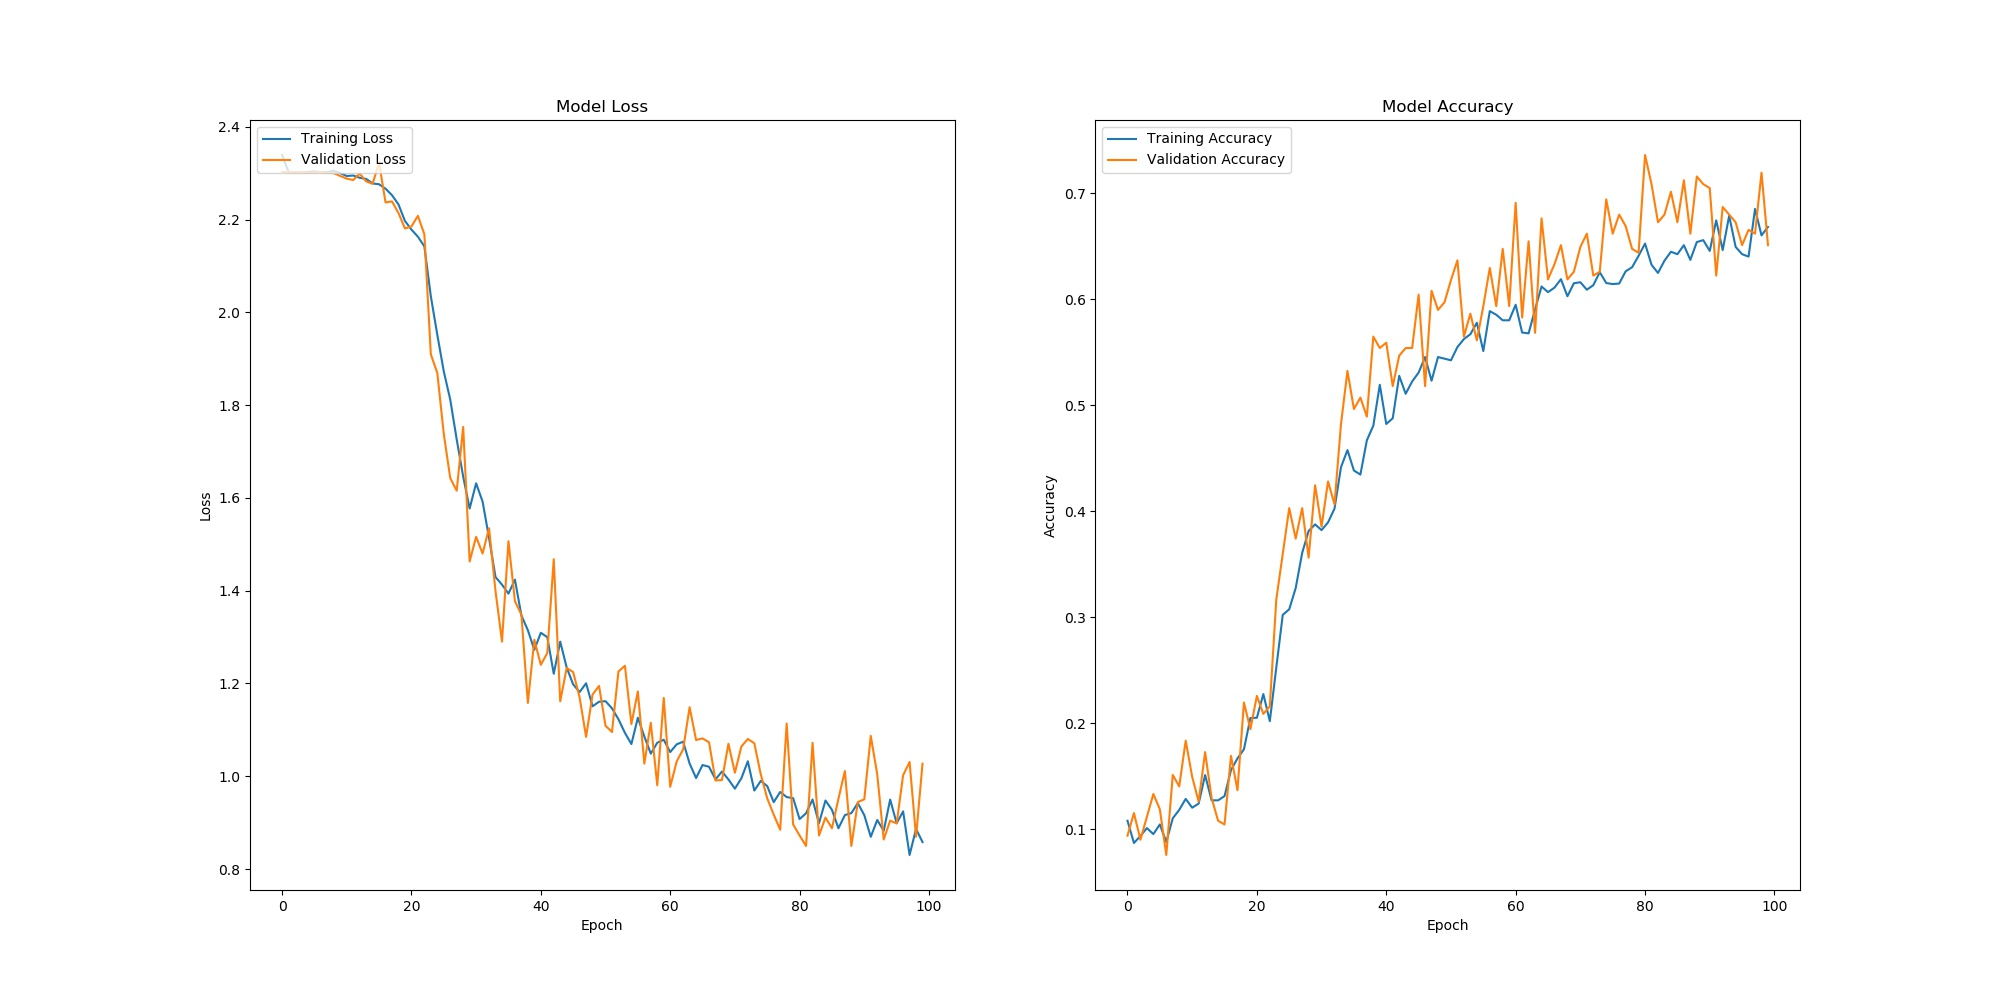
\includegraphics[width=\linewidth]{eval/noDropouttrainingHistory}
        \caption{No Dropout Training History}
        \label{fig:NoDropoutExperiment}
	\end{subfigure}
	\begin{subfigure}{\textwidth}
		\centering
        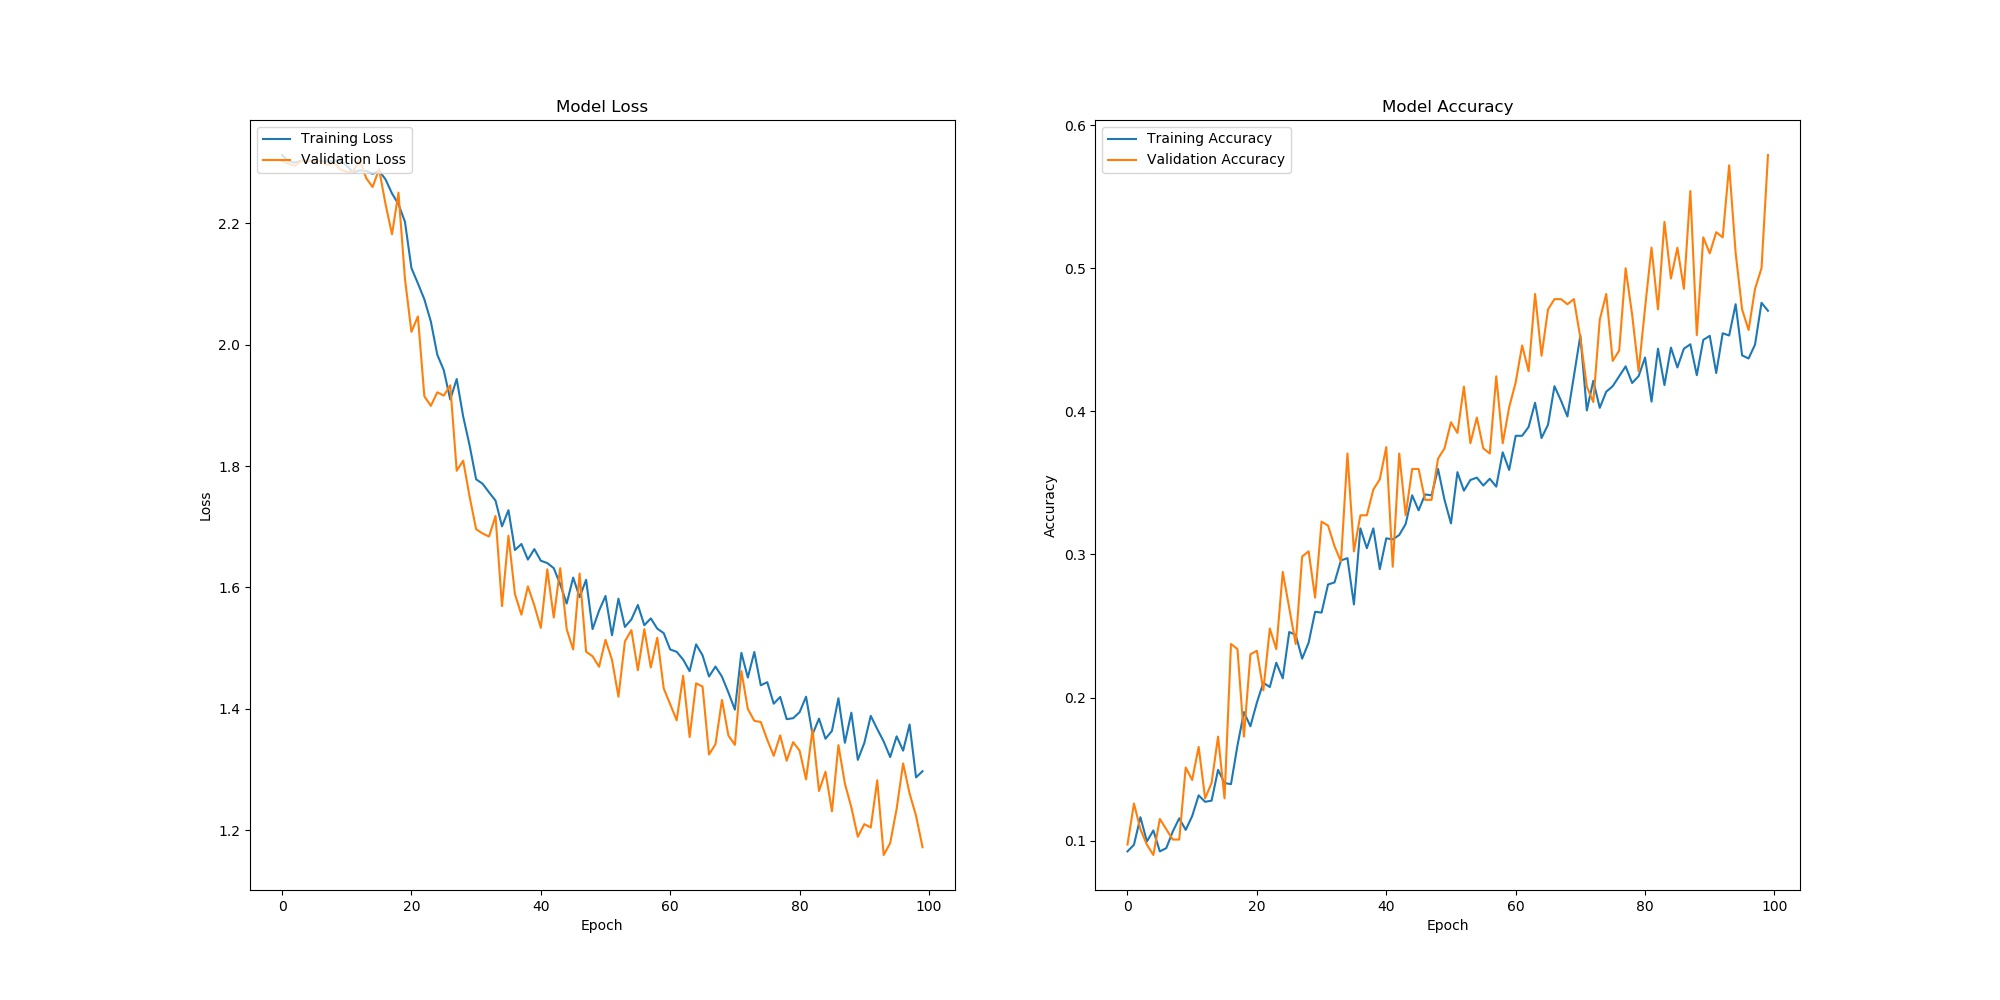
\includegraphics[width=\linewidth]{eval/AugtrainingHistory}
        \caption{Dropout Training History}
        \label{fig:DropoutExperiment}
	\end{subfigure}
	\caption{Results of the Dropout Experiment}
    \label{fig:DropoutExperimentResults}
\end{figure}

From the training plots within Figure \ref{fig:DropoutExperimentResults}, it is clear that dropout has slightly combatted overfitting with respect to this knot classification task. When no dropout is applied, the model's validation loss violently oscillates around the training loss for the entire 100 epochs of training. Although there is no obvious sign of overfitting, the instability of the validation loss value on every epoch reveals that the model may be prone to overfitting if left to train for more epochs. However, with dropout applied, the model's validation loss actually decreases more than the training loss for the whole 100 epochs of training, meaning the model has a higher level of generalisation.

Both of these experiments show that data augmentation and dropout, particularly data augmentation, have successfully combatted the prevalent issue of overfitting.

\section{What is the final performance of the classifier?}
After exploring what features affect classification and what techniques combat overfitting, it was time to pick a model to convert into a Core ML model that could be integrated in the iOS application, and then evaluate the iOS application's final classification performance.
The model that was picked to be integrated in the iOS application was the model with the training history from Figure \ref{fig:AugExperiment}.
This model was picked because its architecture integrated both data augmentation and dropout which were both shown to alleviate the problem of overfitting, its architecture was the medium model architecture which was shown to contain an appropriate number of training parameters for this classification task and the model was trained and validated on the full datasets.
Also, the model's training history reveals that the model had achieved the highest training and validation accuracy and the lowest training and validation loss in the project so far, which was desirable when aiming to evaluate the final classification performance.
After converting this model to a Core ML model and integrating it into the Knot Classifier iOS app, each knot was then tied in both types of climbing rope used in the controlled dataset and the application was used to classify the knots.
Each knot was captured by the app in 36 different scenarios. 
Each knot was tied in two different types of rope, each knot was captured at 0 or 180 degrees of z-axis rotation and 90 or 270 degrees of z-axis rotation, each knot was tied at three different tensions and each knot was captured in three different lighting conditions, giving a grand total of 36 observations for each knot.
Overall the application gave 360 top-3 classifications for 10 knots that were observed 36 times each.
For a valid result, it was important to capture the application's classification labels exactly the same number of times per knot.
The confusion matrix that was created from the true labels and the top predicted labels given by the application is shown in Figure \ref{fig:ConfusionMatrix}.

\begin{figure}
	\centering
	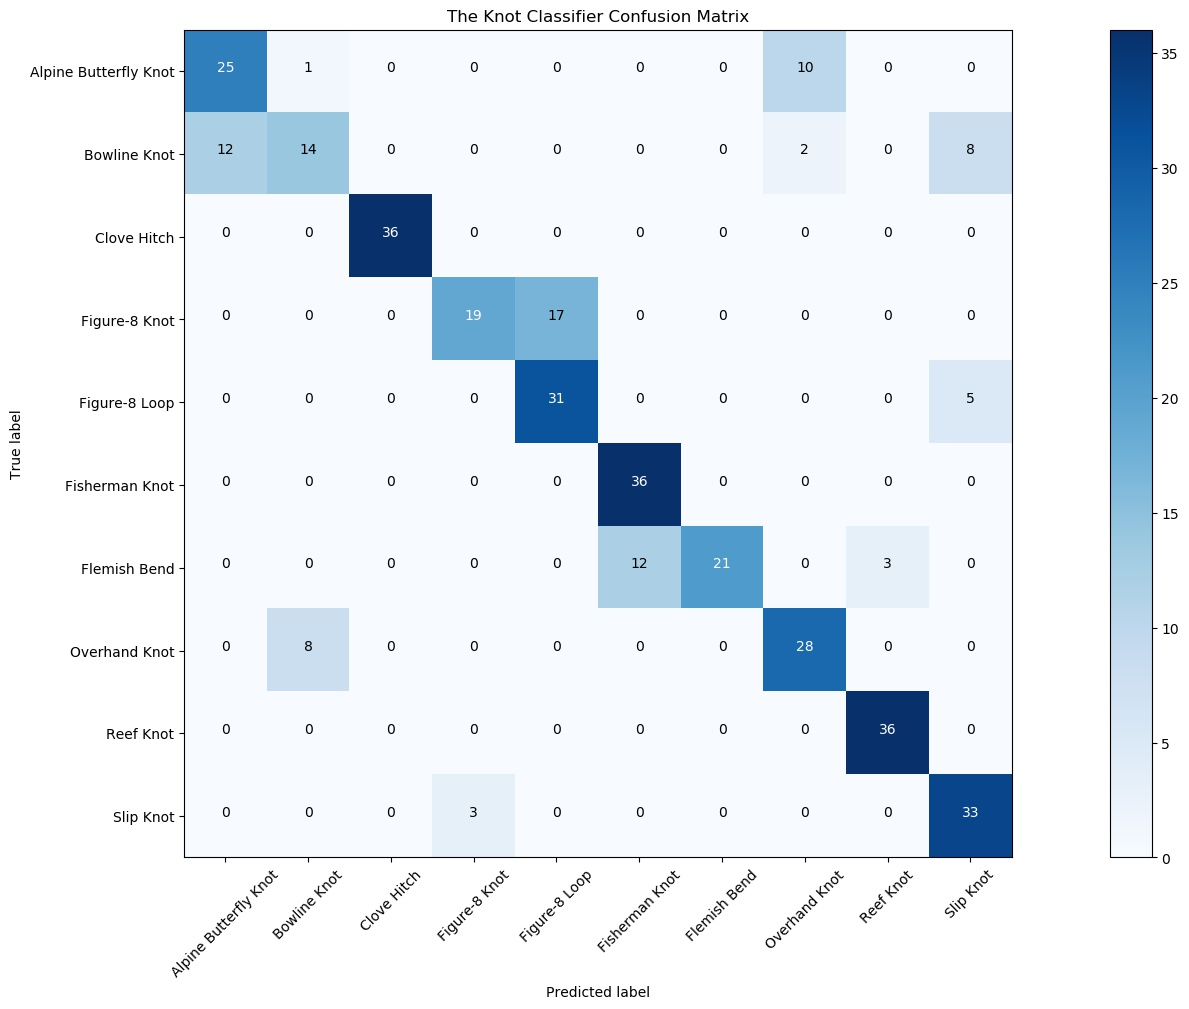
\includegraphics[scale=0.4]{confusionMatrix}
	\caption{Confusion Matrix for The Knot Classifier}
	\label{fig:ConfusionMatrix}
\end{figure}

Figure \ref{fig:ConfusionMatrix} shows that the final classification accuracy was 77.5\%.
For a 10-class classification problem such as this one, this accuracy is extremely promising.
Furthermore, when a knot is misclassified, a knot of similar of topology is classified instead.
For example, when a loop knot such as the bowline knot is misclassified, it is classified instead as either an alpine butterfly knot or a slip knot which are both also loop knots.
This result is extremely encouraging, as it shows the classifier has learnt certain similarities in the topology of the knots and has thus grouped knots together by their respective topology.

\section{Evaluation Conclusion}
After acknowledging the results of this evaluation, it can be concluded that it is certainly possible to classify knots with convolutional neural networks, if those convolutional neural networks have been trained on an appropriate dataset.
Furthermore, the problem of overfitting can be minimised with data augmentation on the training dataset and an incorporation of dropout in the convolutional neural network model architecture.
However, a crucial deciding factor in the classification performance is the number of trainable parameters in the chosen neural network model. Either too many or too few can severely hamper the classification results. Hence, a lot of time dedicated to the implementation of the model architecture is required.

It can also be concluded that the Knot Classifier iOS application served as an effective interface with which the trained convolutional neural network could be used in real-time, as it achieved a classification accuracy of 77.5\% across all 10 knot classes. The iOS application successfully provides the functionality of the knot classifier in even the most remote environments without power and access to a desktop computer.

\subsection{Potential Flaws}
One glaring potential flaw in the evaluation was the small size of the training and validation datasets used to train and validate all of the neural networks.
The size of the training datasets limited the generalisation of the models and the size of the validation datasets limited the conclusions of the evaluation.
For example, the final evaluation of the classifier within the iOS application was done with only 360 samples.
If this evaluation was done with more samples, the final accuracy obtained would be far more convincing and far more representative of the classification performance.

Another flaw in the evaluation was discovered in the t-SNE visualisation.
In the knotClassifier.py script, code that generates a working and correct t-SNE plot was implemented.
However, and rather unfortunately, the t-SNE visualisation plots that were generated for all of the experiments did not show enough grouping or clustering to be of any value to conclude findings from the experiments, and so they had to be ignored.
It is suspected that this may have happened due to the perplexity and epsilon values used, as these hyperparameters can significantly alter the visualisation plot generated by the t-SNE algorithm \cite{wattenberg2016how}.

Upon reflection, another flaw was discovered across all of the experiments.
This flaw was the similarity between the validation and training datasets.
Of course, the training and validation datasets were different, but for example, the same climbing rope and backgrounds were used for the majority of images in both datasets.
The addition of the wild dataset images in the training and validation datasets was an attempt to eliminate this flaw, but it was perhaps not enough in retrospect.
It could have been wise to also perform experiments with a validation dataset that was entirely foreign to the training dataset in order to obtain a more authentic picture of the models' generalisation.
Although, having said this, in evaluating machine learning models there is always a fine line between preparing datasets that are too similar or too different.
If the datasets are too similar, the models may show a better level of generalisation to the validation data than they are worthy of.
However, if the datasets are too different, the models' true learned representations of the training data may go unnoticed.   


%---------------------------------------------

% CONCLUSION

\chapter{Conclusion}

In conclusion, this dissertation has discussed in great detail, the design and implementation of an image classifier that was based on relevant academic literature.
The final product was an iOS application that could achieve real-time knot classification.
Furthermore, the convolutional neural network behind the classification was trained and validated on a comprehensive dataset that was designed and implemented with many different features of knots in mind.
During the evaluation, it was then revealed that the iOS application could reach a classification accuracy of 77.5\% and much useful insight into the features that are important to consider when building a classifier was provided.

\section{Future Work}

\subsubsection{Expanding the Datasets}
A definite consideration for future work is to expand the controlled and wild datasets that were used to train and validate the convolutional neural networks.
Only two types of climbing rope were used in the controlled dataset, which lead to a classifier that was accustomed to correctly classifying knots tied in climbing rope, but this may not necessarily be the case for knots tied in other materials such as ribbon. So, a way of making a more robust classifier could include training the neural networks on images of knots tied in many more diverse materials.

\subsubsection{Classifying More Knots}
This project developed software capable of classifying ten types of knot. Although this is a reasonable amount of knots to classify, a strong avenue of future work could focus on increasing the number of classifiable knots. Obviously, there are many more knots than ten, and ten knots could never possibly encompass the full spectrum of knot topology. Therefore, a natural progression towards building a more comprehensive knot classifier would be to include more knots.

\subsubsection{Application Usability}
The iOS application performed extremely impressive real-time classification. However, if the project were to continue into the future, offline classification capabilities would also be added to the application. In other words, instead of just being able to classify knots through the real-time images being provided by the device's camera, future work could aim to allow users to also classify previous pictures of knots that had been stored within the device's camera roll. This would increase the application's usability in certain situations, such as denied access to a device's camera.

\subsubsection{Classifying More Knot Features}
Currently, only the knot topology itself is classified. However, it may be advantageous and useful to also attempt to classify more features about the knot, such as the tension it was tied to or the material it was tied in.

\subsubsection{Knot Generation \& Manipulation}
A final and very exciting possibility of future work could involve the integration of generative adversarial networks into the project.
Generative adversarial networks, also known as GANs, are capable of generating alternative and modified images from an originally supplied image \cite{Goodfellow:2014:GAN:2969033.2969125}.
In the context of this project, that could open up many new and fascinating research opportunities.
For example, picture a situation in which a mountain climber is using the iOS application to classify a figure-8 loop knot in the hopes of getting a confirmation. 
Imagine that the climber had correctly tied the figure-8 loop, however, the climber had tied it at an inappropriate tension that was too loose.
It may be possible for a GAN to return a modified image of the same knot tied at the correct tension to serve as an aid to the climber after the knot was classified to have been tied at a tension that was too loose.

\section{Acknowledgements}

Firstly, I wish to thank Dr John Williamson for his invaluable supervision and engaging conversations throughout the academic year.
\\\\
Finally, I wish to thank every developer who worked on every piece of open-source software I have used in this project.
The results of this project truly reflect the power and efforts of open-source collaboration. 

%---------------------------------------------

%%%%%%%%%%%%%%%%
%              %
%  APPENDICES  %
%              %
%%%%%%%%%%%%%%%%
\begin{appendices}

\chapter{Running the Programs}
An example of running the knotClassifier.py script from the command line follows:
\begin{verbatim}
      > python knotClassifier.py
\end{verbatim}
This will train the medium-sized convolutional neural network with no data augmentation on data within the dataResized folder contained in the same directory.
\begin{verbatim}
      > python knotClassifier.py -a
\end{verbatim}
This will train the medium-sized convolutional neural network with data augmentation on data within the dataResized folder contained in the same directory.
\begin{verbatim}
      > python knotClassifier.py -a -s
\end{verbatim}
This will train the small-sized convolutional neural network with data augmentation on data within the dataResized folder contained in the same directory.
\begin{verbatim}
      > python knotClassifier.py -a -l
\end{verbatim}
This will train the large-sized convolutional neural network with data augmentation on data within the dataResized folder contained in the same directory.

An example of running the ResizeDataset.py script from the command line follows:
\begin{verbatim}
      > python ResizeDataset.py ./data 500 500
\end{verbatim}
This will resize all data within the 'data' directory to 500 pixels by 500 pixels. Please note that only .jpg and .png files can be resized.

An example of running the convertModel.py script from the command line follows:
\begin{verbatim}
      > python convertModel.py
\end{verbatim}
This will convert a HDF5 model called 'first\_try.h5' located within the same directory to a Core ML model called 'knotClassifier.mlmodel'. The Core ML model will then be saved in the same directory.

\chapter{The Knots}
\label{appendix:Knots}
On the following page, there is a figure containing images of:
\begin{itemize}
	\item The Alpine Butterfly Knot
	\item The Bowline Knot
	\item The Clove Hitch
	\item The Figure-8 Knot
	\item The Figure-8 Loop
	\item The Fisherman's Knot
	\item The Flemish Bend
	\item The Overhand Knot
	\item The Reef Knot
	\item The Slip Knot
\end{itemize}
\begin{figure}[h!]
\begin{subfigure}{.5\textwidth}
  \centering
  \includegraphics[width=.7\linewidth]{ABK}
  \caption{Alpine Butterfly Knot}
  \label{fig:ABK}
\end{subfigure}%
\begin{subfigure}{.5\textwidth}
  \centering
  \includegraphics[width=.7\linewidth]{Bowline}
  \caption{Bowline Knot}
  \label{fig:Bowline}
\end{subfigure}
\begin{subfigure}{.5\textwidth}
  \centering
  \includegraphics[width=.7\linewidth]{CloveHitch}
  \caption{Clove Hitch}
  \label{fig:CloveHitch}
\end{subfigure}
\begin{subfigure}{.5\textwidth}
  \centering
  \includegraphics[width=.7\linewidth]{Fig8}
  \caption{Figure-8 Knot}
  \label{fig:Fig8Knot}
\end{subfigure}
\begin{subfigure}{.5\textwidth}
  \centering
  \includegraphics[width=.7\linewidth]{Fig8Loop}
  \caption{Figure-8 Loop}
  \label{fig:Fig8Loop}
\end{subfigure}
\begin{subfigure}{.5\textwidth}
  \centering
  \includegraphics[width=.7\linewidth]{Fisherman}
  \caption{Fisherman's Knot}
  \label{fig:Fisherman}
\end{subfigure}
\begin{subfigure}{.5\textwidth}
  \centering
  \includegraphics[width=.7\linewidth]{Flemish}
  \caption{Flemish Bend}
  \label{fig:Flemish}
\end{subfigure}
\begin{subfigure}{.5\textwidth}
  \centering
  \includegraphics[width=.7\linewidth]{Overhand}
  \caption{Overhand Knot}
  \label{fig:Overhand}
\end{subfigure}
\begin{subfigure}{.5\textwidth}
  \centering
  \includegraphics[width=.7\linewidth]{Reef}
  \caption{Reef Knot}
  \label{fig:Reef}
\end{subfigure}
\begin{subfigure}{.5\textwidth}
  \centering
  \includegraphics[width=.7\linewidth]{Slip}
  \caption{Slip Knot}
  \label{fig:Slip}
\end{subfigure}
\caption{Knots}
\label{fig:knots}
\end{figure}

\chapter{The Small Convolutional Neural Network Model}
\label{appendix:SmallModel}
The python code for the small model architecture is given below:
\begin{lstlisting}
# SMALL CNN MODEL
if args.small:
    
    print 'You are using the small CNN model architecture'
    
    model = Sequential()
    
    model.add(Conv2D(32, (3, 3), input_shape=input_shape))
    model.add(Activation('relu'))
    model.add(Conv2D(32, (3, 3)))
    model.add(Activation('relu'))
    model.add(MaxPooling2D(pool_size=(2, 2)))
    
    model.add(Conv2D(32, (3, 3)))
    model.add(Activation('relu'))
    model.add(Conv2D(32, (3, 3)))
    model.add(Activation('relu'))
    model.add(MaxPooling2D(pool_size=(2, 2)))
    
    model.add(Conv2D(64, (3, 3)))
    model.add(Activation('relu'))
    model.add(Conv2D(64, (3, 3)))
    model.add(Activation('relu'))
    model.add(MaxPooling2D(pool_size=(2, 2)))
    
    model.add(Conv2D(64, (3, 3)))
    model.add(Activation('relu'))
    model.add(Conv2D(64, (3, 3)))
    model.add(Activation('relu'))
    model.add(MaxPooling2D(pool_size=(2, 2)))
    
    model.add(Dropout(0.5))
    
    model.add(Flatten())
    model.add(Dense(32))
    model.add(Activation('relu'))
    model.add(Dropout(0.5))
    model.add(Dense(10))
    model.add(Activation('softmax'))
    
    model.compile(loss='categorical_crossentropy',
                  optimizer='adam',
                  metrics=['accuracy'])
    
    print model.summary()
\end{lstlisting}

\chapter{The Medium Convolutional Neural Network Model}
\label{appendix:MediumModel}
The python code for the medium model architecture is given below:
\begin{lstlisting}
# MEDIUM CNN MODEL
else:
    
    print 'You are using the medium CNN model architecture'
    
    model = Sequential()
    
    model.add(Conv2D(32, (3, 3), input_shape=input_shape))
    model.add(Activation('relu'))
    model.add(MaxPooling2D(pool_size=(2, 2)))
    
    model.add(Conv2D(32, (3, 3)))
    model.add(Activation('relu'))
    model.add(MaxPooling2D(pool_size=(2, 2)))
    
    model.add(Conv2D(64, (3, 3)))
    model.add(Activation('relu'))
    model.add(MaxPooling2D(pool_size=(2, 2)))
    
    model.add(Dropout(0.5))
    
    model.add(Flatten())
    model.add(Dense(64))
    model.add(Activation('relu'))
    model.add(Dropout(0.5))
    model.add(Dense(10))
    model.add(Activation('softmax'))
    
    model.compile(loss='categorical_crossentropy',
                  optimizer='adam',
                  metrics=['accuracy'])
    
    print model.summary()
\end{lstlisting}


\chapter{The Large Convolutional Neural Network Model}
\label{appendix:LargeModel}
The python code for the large model architecture is given below:
\begin{lstlisting}
# LARGE CNN MODEL
elif args.large:
    
    print 'You are using the large CNN model architecture'
    
    model = Sequential()
    
    model.add(Conv2D(32, (3, 3), input_shape=input_shape))
    model.add(Activation('relu'))
    model.add(Conv2D(32, (3, 3)))
    model.add(Activation('relu'))
    model.add(MaxPooling2D(pool_size=(2, 2)))
    
    model.add(Conv2D(64, (3, 3)))
    model.add(Activation('relu'))
    model.add(Conv2D(64, (3, 3)))
    model.add(Activation('relu'))
    model.add(MaxPooling2D(pool_size=(2, 2)))
    
    model.add(Dropout(0.5))
    
    model.add(Flatten())
    model.add(Dense(128))
    model.add(Activation('relu'))
    model.add(Dense(64))
    model.add(Activation('relu'))
    model.add(Dropout(0.5))
    model.add(Dense(10))
    model.add(Activation('softmax'))
    
    model.compile(loss='categorical_crossentropy',
                  optimizer='adam',
                  metrics=['accuracy'])
    
    print model.summary()
\end{lstlisting}

\chapter{Keras to Core ML Model Conversion}
\label{appendix:KerastoCoreML}
\begin{lstlisting}

# IMPORT STATEMENTS

from keras.models import load_model
import coremltools

# -----------------------------------------------------------

# MODEL CONVERSION

model = load_model('first_try.h5')
classes = ['Alpine Butterfly Knot','Bowline Knot', 'Clove Hitch', 
           'Figure-8 Knot', 'Figure-8 Loop', 'Fisherman Knot', 
           'Flemish Bend', 'Overhand Knot', 'Reef Knot', 'Slip Knot']

coreml_model = coremltools.converters.keras.convert(model,
                                                    input_names=['image'],
                                                    image_input_names='image',
                                                    class_labels=classes,
                                                    image_scale=1/255.)

# -----------------------------------------------------------

# ADD COREML MODEL INFORMATION

coreml_model.author = 'Joseph Cameron'
coreml_model.license = 'MIT'
coreml_model.short_description = 'This model classifies knots.'
coreml_model.input_description['image'] = 'A 150x150 pixel image.'
coreml_model.output_description['output1'] = 'A one-hot MultiArray where the array index with the largest float value between 0 and 1 is the recognised knot.'

# -----------------------------------------------------------

# SAVE THE COREML MODEL

coreml_model.save('knotClassifier.mlmodel')

\end{lstlisting}


\chapter{ViewController.swift}
\label{appendix:SwiftViewController}
\begin{lstlisting}[language=swift]
//
//  ViewController.swift
//  The Knot Classifier
//
//  Created by Joseph Cameron on 23/01/2018.
//  Copyright © 2018 Joseph Cameron. All rights reserved.
//
import UIKit
import AVKit
import Vision

class ViewController: UIViewController, AVCaptureVideoDataOutputSampleBufferDelegate {
    
    @IBOutlet weak var predictionOutput: UILabel!
    
    override func viewDidLoad() {
        super.viewDidLoad()
        
        // Start up the camera here
        
        let captureSession = AVCaptureSession()
        captureSession.sessionPreset = .photo // Collapses the camera's view on the screen.
        guard let captureDevice = AVCaptureDevice.default(for: .video) else { return }
        guard let captureInput = try? AVCaptureDeviceInput(device: captureDevice) else { return }
        captureSession.addInput(captureInput)
        captureSession.startRunning()
        let previewLayer = AVCaptureVideoPreviewLayer(session: captureSession)
        view.layer.addSublayer(previewLayer)
        previewLayer.frame = view.frame
        
        //----------------------------------------------------------------------------------
        
        // Now, we analyse the images
        
        let dataOutput = AVCaptureVideoDataOutput()
        dataOutput.setSampleBufferDelegate(self, queue: DispatchQueue(label: "videoQueue"))
        captureSession.addOutput(dataOutput)
        
    }
    
    func captureOutput(_ output: AVCaptureOutput, didOutput sampleBuffer: CMSampleBuffer, from connection: AVCaptureConnection) {
        
        guard let pixelBuffer: CVPixelBuffer = CMSampleBufferGetImageBuffer(sampleBuffer) else { return }
        
        // Specify knotClassifier.mlmodel as the model
        guard let model = try? VNCoreMLModel(for: knotClassifier().model) else { return }
        
        // Create request for CoreML
        let request = VNCoreMLRequest(model: model) { (finishedReq, err) in
            
            // Get classification results from knotClassifier.mlmodel
            guard let results = finishedReq.results as? [VNClassificationObservation] else { return }
            
            // Get the top-3 VNClassificationObservations
            let top3 = results.prefix(through: 2).map { classification in return String(format: " %@ (%.2f)", classification.identifier, classification.confidence) }
            
            // Does not update the label without a dispatch to the main thread.
            DispatchQueue.main.async {
                // Display each classification and probability on its own line, in order of probability
                self.predictionOutput.text = top3.joined(separator: "\n")
            }
            
        }
        
        try? VNImageRequestHandler(cvPixelBuffer: pixelBuffer, options: [:]).perform([request])
        
    }

    override func didReceiveMemoryWarning() {
        super.didReceiveMemoryWarning()
        // Dispose of any resources that can be recreated.
    }


}
\end{lstlisting}


\end{appendices}

%%%%%%%%%%%%%%%%%%%%
%   BIBLIOGRAPHY   %
%%%%%%%%%%%%%%%%%%%%

\bibliographystyle{plain}
\bibliography{bib}

\end{document}
